%% Generated by Sphinx.
\def\sphinxdocclass{report}
\documentclass[a4paper,11pt,english,openany,oneside]{sphinxmanual}
\ifdefined\pdfpxdimen
   \let\sphinxpxdimen\pdfpxdimen\else\newdimen\sphinxpxdimen
\fi \sphinxpxdimen=.75bp\relax
\ifdefined\pdfimageresolution
    \pdfimageresolution= \numexpr \dimexpr1in\relax/\sphinxpxdimen\relax
\fi
\newdimen\sphinxremdimen\sphinxremdimen = 11pt
%% let collapsible pdf bookmarks panel have high depth per default
\PassOptionsToPackage{bookmarksdepth=5}{hyperref}

\PassOptionsToPackage{booktabs}{sphinx}

\PassOptionsToPackage{warn}{textcomp}


\usepackage{cmap}
\usepackage{xeCJK}
\usepackage{amsmath,amssymb,amstext}
\usepackage{babel}



\setmainfont{FreeSerif}[
  Extension      = .otf,
  UprightFont    = *,
  ItalicFont     = *Italic,
  BoldFont       = *Bold,
  BoldItalicFont = *BoldItalic
]
\setsansfont{FreeSans}[
  Extension      = .otf,
  UprightFont    = *,
  ItalicFont     = *Oblique,
  BoldFont       = *Bold,
  BoldItalicFont = *BoldOblique,
]
\setmonofont{FreeMono}[Scale=0.9,
  Extension      = .otf,
  UprightFont    = *,
  ItalicFont     = *Oblique,
  BoldFont       = *Bold,
  BoldItalicFont = *BoldOblique,
]



\usepackage[Sonny]{fncychap}
\usepackage[,numfigreset=1,mathnumfig,mathnumsep={.}]{sphinx}

\fvset{fontsize=\small,formatcom=\xeCJKVerbAddon}
\usepackage{geometry}


% Include hyperref last.
\usepackage{hyperref}
% Fix anchor placement for figures with captions.
\usepackage{hypcap}% it must be loaded after hyperref.
% Set up styles of URL: it should be placed after hyperref.
\urlstyle{same}

\addto\captionsenglish{\renewcommand{\contentsname}{目录}}

\usepackage{sphinxmessages}
\setcounter{tocdepth}{3}
\setcounter{secnumdepth}{3}


\usepackage{longtable}
\usepackage{booktabs}    

% ===== 中文支持 =====
\usepackage{xeCJK}
\usepackage[fontset=windows]{ctex}

% ===== 页面边距与页眉空间分配 =====
\usepackage{geometry}
\geometry{
    left=25mm,
    right=25mm,
    top=30mm,
    bottom=25mm,
    headheight=25pt, % 留足页眉高度
    headsep=8mm      % 页眉与正文的距离
}

% ===== 图片路径 =====
\graphicspath{{images/}}

% ===== 禁止图表浮动 =====
\usepackage{float}
\usepackage{placeins}

\makeatletter
\def\fps@figure{H}
\def\fps@table{H}
\def\fps@sphinxfigure{H}
\def\fps@sphinxTable{H}
\makeatother

% ==== 强制图片后换行 ===
\usepackage{etoolbox}
\AtEndEnvironment{figure}{\par\noindent}
\AtEndEnvironment{sphinxfigure}{\par\noindent}

% ===== 代码高亮 =====
\usepackage{listings}

% ===== PDF书签 =====
\usepackage{bookmark}

% ===== 自定义变量 =====
\newcommand{\docversion}{V01}
\newcommand{\docname}{Zu15\&Zu35服务手册}

% ===== 页眉页脚 (恢复 LastPage 避免??) =====
\usepackage{fancyhdr}
\usepackage{lastpage} 

% 1. 重定义 Sphinx 的正文页样式 (normal)
\fancypagestyle{normal}{
    \fancyhf{}  
    \fancyhead[L]{\raisebox{0.05cm}{
\includegraphics[height=0.5cm]{Logo.png}}}
    \fancyhead[R]{\nouppercase{\leftmark}}  
    \fancyfoot[L]{版本： \docversion}
    % 使用最稳定的 LastPage
    \fancyfoot[C]{\thepage/\pageref*{LastPage}}
    \fancyfoot[R]{\docname}
    \renewcommand{\headrulewidth}{0.4pt} 
    \renewcommand{\footrulewidth}{0.4pt}
}

% 2. 重定义 Sphinx 的章节起始页样式 (plain)
\fancypagestyle{plain}{
    \fancyhf{}
    \fancyhead[L]{\raisebox{0.05cm}{
\includegraphics[height=0.5cm]{Logo.png}}}
    \fancyhead[R]{\nouppercase{\leftmark}} 
    \fancyfoot[L]{版本： \docversion}
    \fancyfoot[C]{\thepage/\pageref*{LastPage}}
    \fancyfoot[R]{\docname}
    \renewcommand{\headrulewidth}{0.4pt}   
    \renewcommand{\footrulewidth}{0.4pt}
}

% ===== 标题样式 =====
\usepackage{titlesec}
\usepackage{xcolor}

% 定义红色
\definecolor{TitleRed}{HTML}{D80C1E}

% 章节间距
\titlespacing*{\chapter}{0pt}{-30pt}{20pt}

% Chapter
\titleformat{\chapter}
{\Huge\bfseries\color{TitleRed}}
{\thechapter}{0.5em}{}

% Section
\titleformat{\section}
{\Large\bfseries\color{TitleRed}}
{\thesection}{0.5em}{}

% Subsection
\titleformat{\subsection}
{\large\bfseries\color{TitleRed}}
{\thesubsection}{0.5em}{}

% Subsubsection
\titleformat{\subsubsection}
{\normalsize\bfseries\color{TitleRed}}
{\thesubsubsection}{0.5em}{}

% ===== 超链接颜色 =====
\usepackage{hyperref}

\hypersetup{
colorlinks=true,
linkcolor=blue,
urlcolor=blue,
citecolor=blue
}

% ===== 所有目录页变黑，正文恢复蓝色 (强力黑盒覆盖版) =====

% 1. 主目录
\let\origsphinxtableofcontents\sphinxtableofcontents
\renewcommand{\sphinxtableofcontents}{
    \begingroup
    \cleardoublepage
    \pagenumbering{Roman}
    \pagestyle{plain} 
    \hypersetup{linkcolor=black}
    \origsphinxtableofcontents
    \clearpage
    \endgroup
    \pagenumbering{arabic}
    \pagestyle{normal}
}

% 2. 图目录
\let\origlistoffigures\listoffigures
\renewcommand{\listoffigures}{
    \begingroup
    \hypersetup{linkcolor=black}
    \origlistoffigures
    \endgroup
}

% 3. 表目录
\let\origlistoftables\listoftables
\renewcommand{\listoftables}{
    \begingroup
    \hypersetup{linkcolor=black}
    \origlistoftables
    \endgroup
}

% ===== 表格样式 =====
\usepackage{colortbl}
\usepackage{longtable}
\usepackage{booktabs}

\definecolor{tableheader}{RGB}{200,0,0}
\definecolor{tableborder}{RGB}{160,160,160}

\arrayrulecolor{tableborder}

% 表头样式
\renewcommand{\sphinxstyletheadfamily}{
\color{white}\bfseries
}

\newcommand{\sphinxstyletheadbackground}{
\rowcolor{tableheader}
}

\appto\sphinxstyletheadfamily{\sphinxstyletheadbackground}

% ===== 表格跨页与宽度控制 =====
\usepackage{tabularx}
\usepackage{ltablex}
\keepXColumns

% 表格自动换行
\renewcommand{\tabularxcolumn}[1]{m{#1}}

% 表格不要超出页边距
\setlength{\LTleft}{0pt}
\setlength{\LTright}{0pt}

% ===== 代码块分页优化 =====
\sphinxsetup{
verbatimwithframe=false
}

\usepackage{tocloft}

% ===== 中文图表名称 =====
\AtBeginDocument{
    \renewcommand{\figurename}{图}
    \renewcommand{\tablename}{表}
    \renewcommand{\listfigurename}{图目录}
    \renewcommand{\listtablename}{表目录}
    
    % 防止图表目录编号和名称重叠
    \setlength{\cftfignumwidth}{3em}
    \setlength{\cfttabnumwidth}{3em}
}



\title{Zu15&Zu35服务手册}
\date{2026 年 05 月 21 日}
\release{V01}
\author{JAKA}
\newcommand{\sphinxlogo}{\vbox{}}
\renewcommand{\releasename}{版本}
\makeindex
\begin{document}

\ifdefined\shorthandoff
  \ifnum\catcode`\=\string=\active\shorthandoff{=}\fi
  \ifnum\catcode`\"=\active\shorthandoff{"}\fi
\fi

\pagestyle{empty}
\begin{titlepage}
    \thispagestyle{empty}
    \centering

\vspace*{1cm}

    % 顶部 JAKA 图片
    
\includegraphics[width=0.3\textwidth]{Logo.png} \\[1cm]

    % 硬件用户手册
    {\bfseries\fontsize{32pt}{38pt}\selectfont 服务手册\par}
    \vspace{1cm}

    % 产品图
    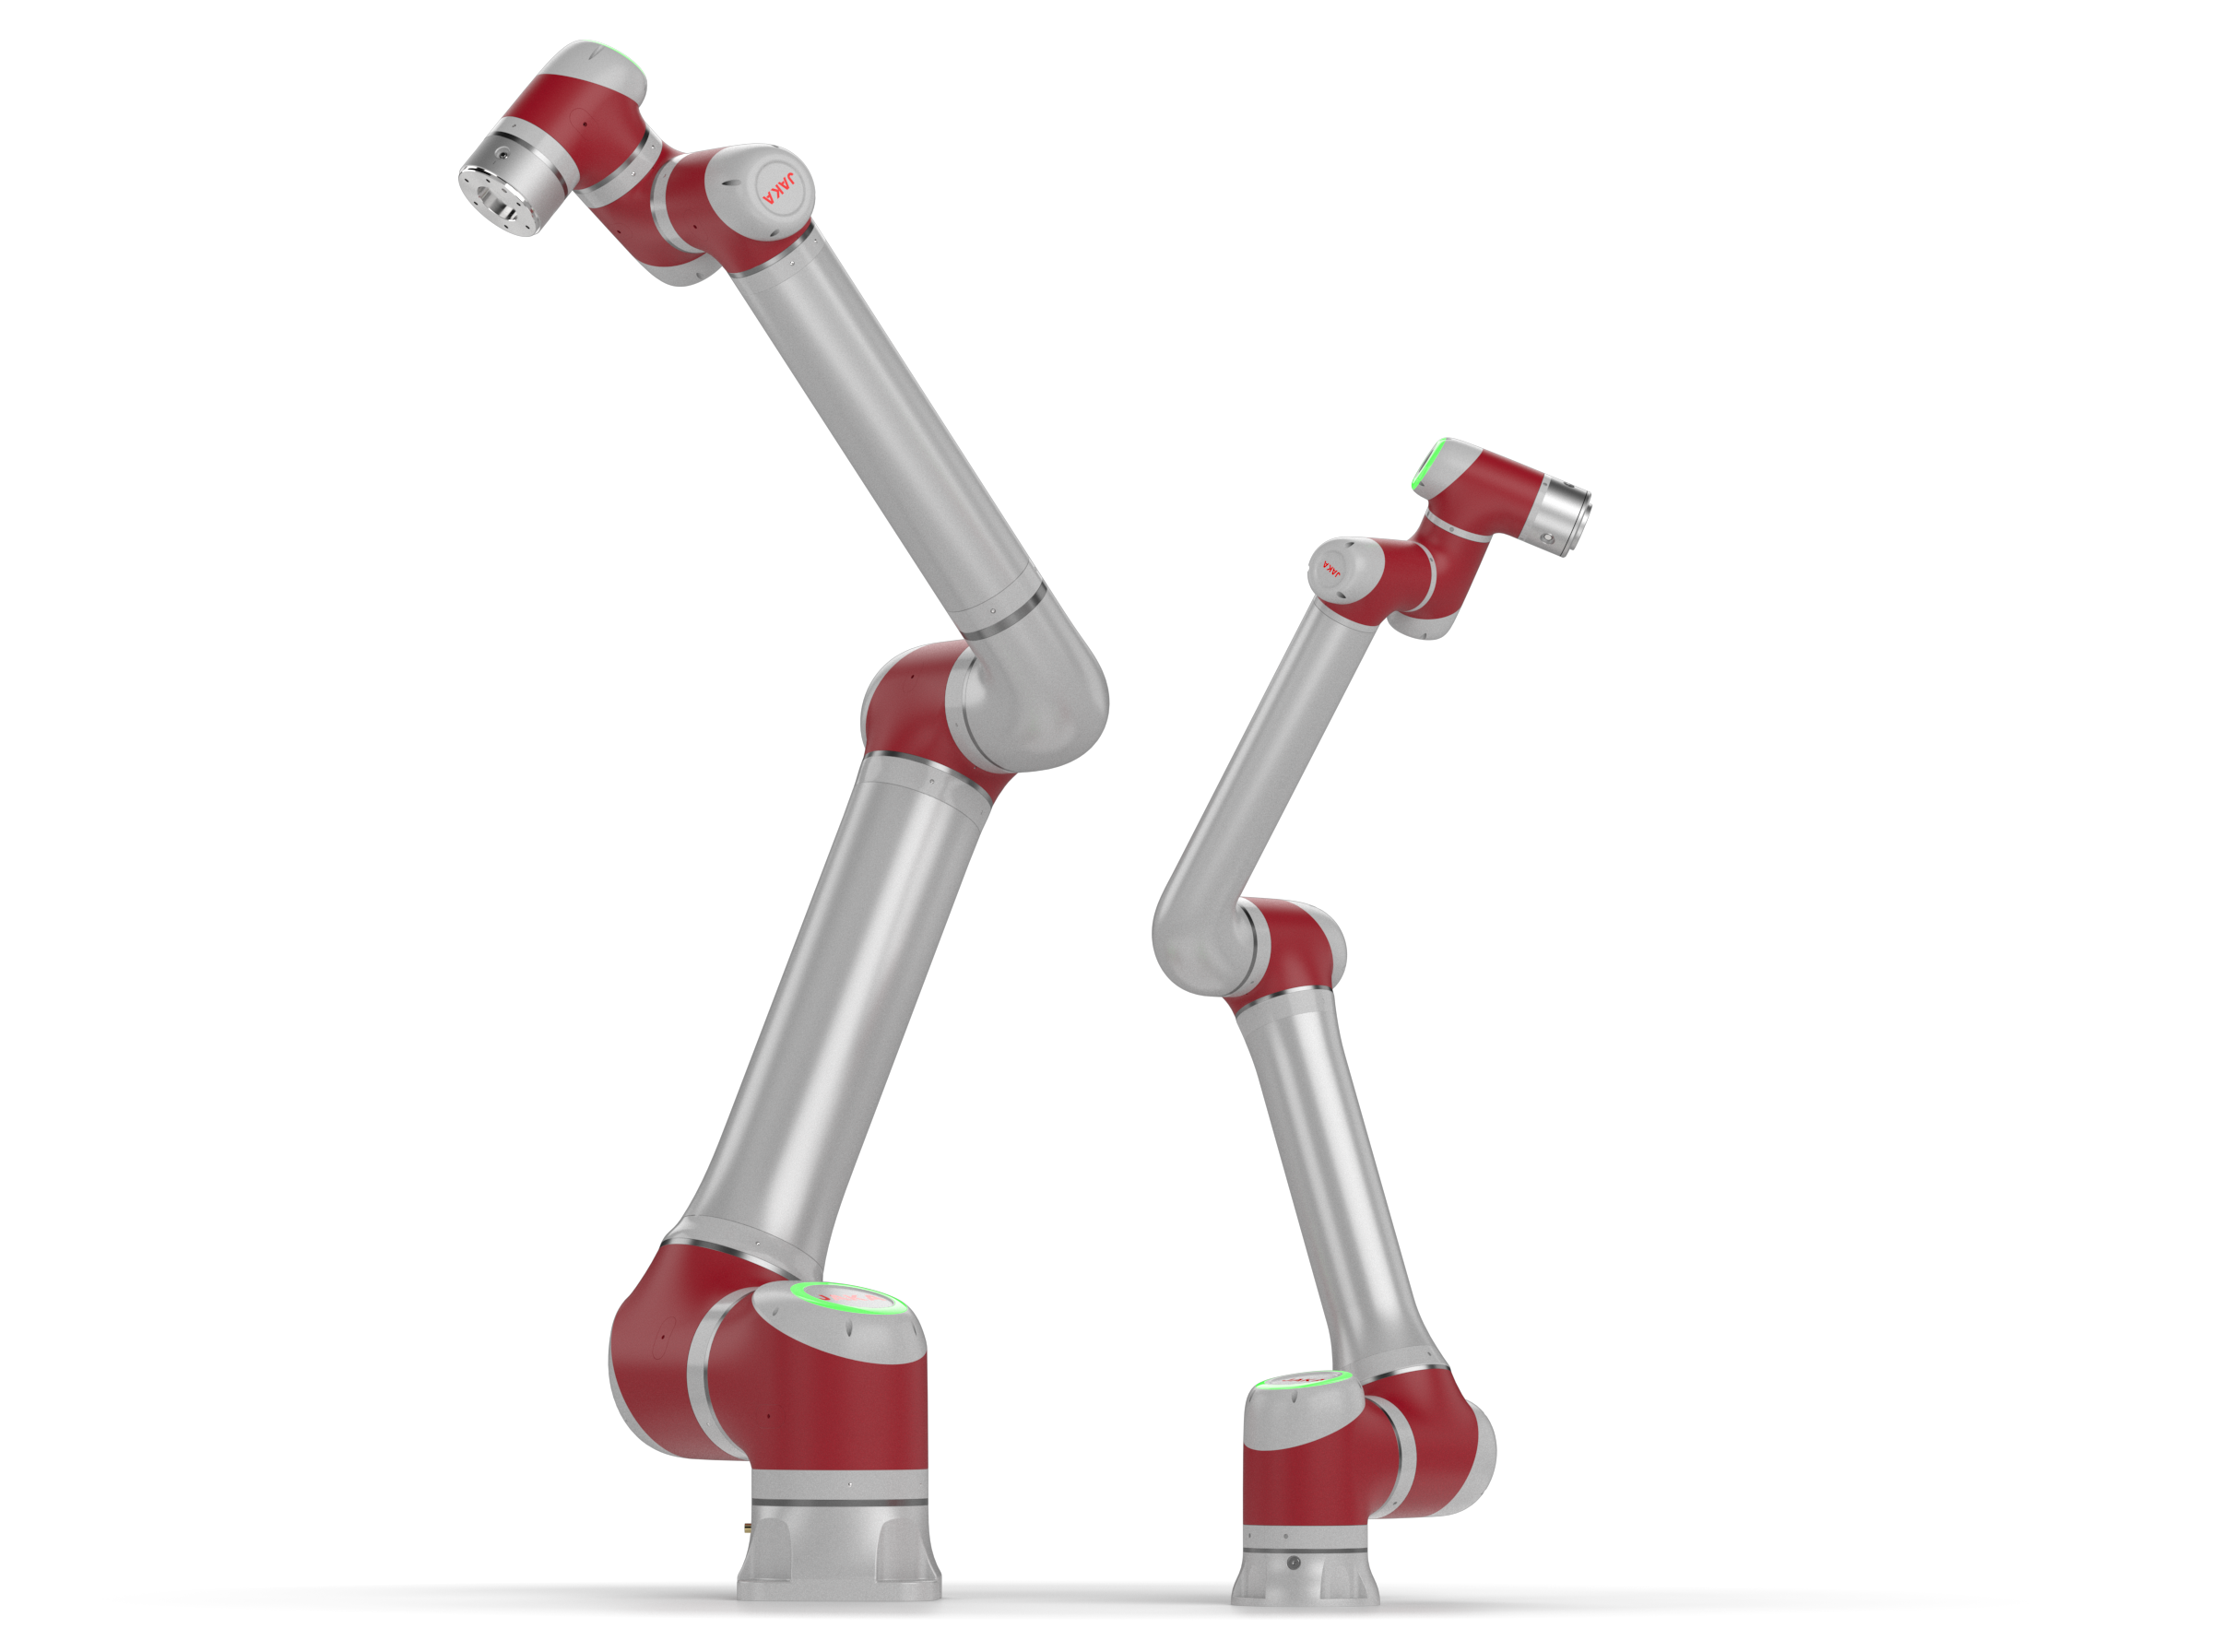
\includegraphics[width=0.8\textwidth]{Zu1535.png} \\[1cm]
    
    % 型号名称
    {\LARGE Zu15 \& Zu35\par}
    \vspace{0.5cm}
    
    % 版本信息
    {\large 翻译版本（zh）\par}
    {\large 文档版本：\docversion\par}

    \vspace{\fill}
    
    % 底部信息（右对齐）
    \begin{flushright}
        \large
        机器人：Zu15，Zu35 \\
        软件：V3.3.8及以上版本Coboπ App \\
    \end{flushright}
    
    \vspace{1cm}
\end{titlepage}
\pagestyle{plain}
\sphinxtableofcontents
\pagestyle{normal}
\phantomsection\label{\detokenize{index::doc}}


\sphinxAtStartPar
本手册是节卡机器人股份有限公司（后文统称为“节卡”或“JAKA”）的专有财产，其版权及解释权归JAKA及其关联公司所有。未经JAKA的书面同意，其他任何方不得以任何形式使用其内容。

\sphinxAtStartPar
JAKA会定期对手册进行修正和完善，其内容可能会更新，恕不另行通知。使用本手册前请认真核对实际产品信息。

\sphinxAtStartPar
本手册适用于JAKA推出的全部产品和/或服务（后文统称为“产品”），手册所包含的信息按产品“现状”提供，受中华人民共和国法律（不包括香港、澳门与台湾地区法律）的约束并依据其解释，在法律允许的最大范围内，本手册不构成JAKA任何形式的明示或暗示的陈述或保证，亦不构成对JAKA有关产品的适销性、适用于特定目的、达到预期效果以及不侵权的保证。JAKA对本手册中仍然可能出现的任何错误、遗漏以及对使用本手册及其所介绍产品而引起的意外或间接伤害概不负责。安装、使用产品前，请仔细阅读本手册。

\sphinxAtStartPar
本手册图片仅供参考，请以实物为准。

\sphinxAtStartPar
若JAKA产品出现被改造或者拆卸的情况，JAKA不负责无偿售后工作。

\sphinxAtStartPar
JAKA提醒用户在使用、维修JAKA机器人时必须使用安全设备，必须遵守安全条款。

\sphinxAtStartPar
JAKA的程序设计者、机器人系统的设计和调试者，必须熟悉JAKA机器人的编程方式和系统应用安装。

\sphinxAtStartPar
\sphinxstylestrong{更多信息}

\sphinxAtStartPar
如果您还想了解更多的产品信息，请扫描下方二维码访问我们的官网www.jaka.com。

\begin{figure}[H]
\centering

\noindent\sphinxincludegraphics{{官网二维码}.png}
\end{figure}

\sphinxstepscope


\chapter{手册概述}
\label{\detokenize{_u624b_u518c_u6982_u8ff0:id1}}\label{\detokenize{_u624b_u518c_u6982_u8ff0::doc}}

\section{关于本手册}
\label{\detokenize{_u624b_u518c_u6982_u8ff0:id2}}
\sphinxAtStartPar
本手册包含以下内容：
\begin{itemize}
\item {} 
\sphinxAtStartPar
机器人的维护与清洁操作

\item {} 
\sphinxAtStartPar
机器人的维修操作

\item {} 
\sphinxAtStartPar
产品故障排查说明

\end{itemize}


\section{手册阅读对象}
\label{\detokenize{_u624b_u518c_u6982_u8ff0:id3}}
\sphinxAtStartPar
本手册面向：
\begin{itemize}
\item {} 
\sphinxAtStartPar
维护人员

\item {} 
\sphinxAtStartPar
集成商

\end{itemize}


\section{参考信息}
\label{\detokenize{_u624b_u518c_u6982_u8ff0:id4}}
\sphinxAtStartPar
本手册中引用的文档：
\begin{itemize}
\item {} 
\sphinxAtStartPar
JAKA Coboπ软件用户手册

\item {} 
\sphinxAtStartPar
JAKA Zu15\&Zu35硬件用户手册

\end{itemize}

\begin{sphinxadmonition}{note}{备注:}
\sphinxAtStartPar
以上文档可从 \sphinxhref{https://www.jaka.com/zh}{JAKA官网} 获得。
\end{sphinxadmonition}


\section{人员要求}
\label{\detokenize{_u624b_u518c_u6982_u8ff0:id5}}
\sphinxAtStartPar
本手册面向用户应：
\begin{itemize}
\item {} 
\sphinxAtStartPar
接受过JAKA的培训并具备机械、了解电子安装/维修/维护工作所需的知识。

\item {} 
\sphinxAtStartPar
接受过应对紧急情况或和异常情况的培训。

\end{itemize}

\sphinxstepscope


\chapter{安全规范}
\label{\detokenize{_u5b89_u5168_u89c4_u8303:id1}}\label{\detokenize{_u5b89_u5168_u89c4_u8303:id2}}\label{\detokenize{_u5b89_u5168_u89c4_u8303::doc}}
\sphinxAtStartPar
本章主要介绍了使用机器人或机器人系统时应遵守的安全原则和规范。用户应仔细阅读本手册的安全方面相关内容，并严格遵守。操作人员应充分认识到机器人系统的复杂性和危险性，应特别注意与警告标志相关的内容。


\section{安全警告标志说明}
\label{\detokenize{_u5b89_u5168_u89c4_u8303:id3}}
\sphinxAtStartPar
本手册的危险等级规定使用如下警示标志进行说明，有关安全的内容，请严格遵守。


\begin{savenotes}\sphinxattablestart
\sphinxthistablewithglobalstyle
\centering
\sphinxcapstartof{table}
\sphinxthecaptionisattop
\sphinxcaption{安全标识说明}\label{\detokenize{_u5b89_u5168_u89c4_u8303:id6}}
\sphinxaftertopcaption
\begin{tabular}[t]{\X{20}{100}\X{80}{100}}
\sphinxtoprule
\begin{varwidth}[t]{\sphinxcolwidth{1}{2}}
\sphinxstyletheadfamily \sphinxAtStartPar
\sphinxstylestrong{标识}
\sphinxbeforeendvarwidth
\end{varwidth}%
&\begin{varwidth}[t]{\sphinxcolwidth{1}{2}}
\sphinxstyletheadfamily \sphinxAtStartPar
\sphinxstylestrong{说明}
\sphinxbeforeendvarwidth
\end{varwidth}%
\\
\sphinxmidrule
\sphinxtableatstartofbodyhook\begin{varwidth}[t]{\sphinxcolwidth{1}{2}}
\sphinxAtStartPar
\sphinxstylestrong{警告：带电}
\sphinxbeforeendvarwidth
\end{varwidth}%
&\begin{varwidth}[t]{\sphinxcolwidth{1}{2}}
\sphinxAtStartPar
这个标志表示可能引发危险的用电情况，若不避免，可导致人员伤害或设备严重损坏。
\sphinxbeforeendvarwidth
\end{varwidth}%
\\
\sphinxhline\begin{varwidth}[t]{\sphinxcolwidth{1}{2}}
\sphinxAtStartPar
\sphinxstylestrong{警告}
\sphinxbeforeendvarwidth
\end{varwidth}%
&\begin{varwidth}[t]{\sphinxcolwidth{1}{2}}
\sphinxAtStartPar
这个标志表示可能引发危险的情况，若不避免，可导致人员伤害或设备严重损坏。
\sphinxbeforeendvarwidth
\end{varwidth}%
\\
\sphinxhline\begin{varwidth}[t]{\sphinxcolwidth{1}{2}}
\sphinxAtStartPar
\sphinxstylestrong{静电释放（ESD）}
\sphinxbeforeendvarwidth
\end{varwidth}%
&\begin{varwidth}[t]{\sphinxcolwidth{1}{2}}
\sphinxAtStartPar
用于表示潜在危险状况，如果对这种状况不加避免，则可能导致产品的严重损坏。
\sphinxbeforeendvarwidth
\end{varwidth}%
\\
\sphinxhline\begin{varwidth}[t]{\sphinxcolwidth{1}{2}}
\sphinxAtStartPar
\sphinxstylestrong{注意}
\sphinxbeforeendvarwidth
\end{varwidth}%
&\begin{varwidth}[t]{\sphinxcolwidth{1}{2}}
\sphinxAtStartPar
这个标志表示重要事实和状况。
\sphinxbeforeendvarwidth
\end{varwidth}%
\\
\sphinxhline\begin{varwidth}[t]{\sphinxcolwidth{1}{2}}
\sphinxAtStartPar
\sphinxstylestrong{备注}
\sphinxbeforeendvarwidth
\end{varwidth}%
&\begin{varwidth}[t]{\sphinxcolwidth{1}{2}}
\sphinxAtStartPar
此标志用于说明附加信息。
\sphinxbeforeendvarwidth
\end{varwidth}%
\\
\sphinxbottomrule
\end{tabular}
\sphinxtableafterendhook\par
\sphinxattableend\end{savenotes}


\section{警告及提醒}
\label{\detokenize{_u5b89_u5168_u89c4_u8303:id4}}
\sphinxAtStartPar
为确保机器人系统安全、稳定运行，所有维护、校准、检修及故障排除工作必须严格遵守本手册及相关服务文档中的安全要求，并符合适用的国家或地区职业安全法规。

\sphinxAtStartPar
维护与维修工作应依据最新版本的服务手册执行，或由已接受节卡学院专业培训的人员进行操作。所有维修操作仅限由节卡授权的系统集成商或节卡技术服务人员实施。涉及部件返修或退回时，应按照服务手册规定的流程和要求进行处理。

\sphinxAtStartPar
在开展维护或维修工作前，必须确认设备处于安全状态，并采取必要的断电、隔离及防护措施。维护完成后，应对所有相关安全功能进行检查与验证，确保其运行正常并满足规定的安全等级要求。

\sphinxAtStartPar
维护与维修工作的目的在于保障机器人系统持续处于正常运行状态，并在发生异常或故障时恢复系统功能。相关工作包括但不限于状态检查、故障诊断、参数校准、部件更换及系统恢复等操作。

\sphinxAtStartPar
未经节卡授权或未获得节卡技术服务人员许可，用户不得擅自对机器人的机械系统、电气系统或安全系统进行修理、改装、参数调整或其他干预操作。任何未经授权的拆卸、修改或维修行为均可能导致设备损坏、安全风险增加，并将导致产品保修失效。

\sphinxAtStartPar
所有维修相关操作及故障排除工作必须由具备相应资质的专业人员执行。

\sphinxAtStartPar
操作机器人时，必须严格遵守以下安全程序及警告事项：


\begin{savenotes}\sphinxattablestart
\sphinxthistablewithglobalstyle
\centering
\sphinxcapstartof{table}
\sphinxthecaptionisattop
\sphinxcaption{通用警告}\label{\detokenize{_u5b89_u5168_u89c4_u8303:id7}}
\sphinxaftertopcaption
\begin{tabular}[t]{\X{20}{100}\X{80}{100}}
\sphinxtoprule
\begin{varwidth}[t]{\sphinxcolwidth{1}{2}}
\sphinxstyletheadfamily \sphinxAtStartPar
\sphinxstylestrong{标识}
\sphinxbeforeendvarwidth
\end{varwidth}%
&\begin{varwidth}[t]{\sphinxcolwidth{1}{2}}
\sphinxstyletheadfamily \sphinxAtStartPar
\sphinxstylestrong{说明}
\sphinxbeforeendvarwidth
\end{varwidth}%
\\
\sphinxmidrule
\sphinxtableatstartofbodyhook\begin{varwidth}[t]{\sphinxcolwidth{1}{2}}

\noindent\sphinxincludegraphics[width=1.5cm]{{触电}.png}
\sphinxbeforeendvarwidth
\end{varwidth}%
&\begin{varwidth}[t]{\sphinxcolwidth{1}{2}}
\sphinxAtStartPar
\sphinxstylestrong{警告：带电}
\begin{itemize}
\item {} 
\sphinxAtStartPar
维修前必须断开控制柜电源，以确保系统完全断电。同时，应断开机器人及控制柜连接的所有电源。

\item {} 
\sphinxAtStartPar
须在切断主电源5分钟后，再进行部件的更换。由于基板及电解电容中存在残留电荷，有触电危险。

\item {} 
\sphinxAtStartPar
在维护期间，必须采取必要的锁定/挂牌（Lockout/Tagout）等安全措施，防止他人误重新接通电源。

\item {} 
\sphinxAtStartPar
在重新上电或恢复系统运行前，必须检查并确认接地连接可靠有效。

\item {} 
\sphinxAtStartPar
拆卸机器人内部部件时，必须遵守 ESD（静电放电）防护规范，防止静电损坏电子元件。

\item {} 
\sphinxAtStartPar
必须防止水、液体或粉尘进入机器人内部，以避免造成设备故障、短路或安全事故。

\item {} 
\sphinxAtStartPar
禁止使用湿手进行作业。

\end{itemize}
\sphinxbeforeendvarwidth
\end{varwidth}%
\\
\sphinxhline\begin{varwidth}[t]{\sphinxcolwidth{1}{2}}

\noindent\sphinxincludegraphics[width=1.5cm]{{危险}.png}
\sphinxbeforeendvarwidth
\end{varwidth}%
&\begin{varwidth}[t]{\sphinxcolwidth{1}{2}}
\sphinxAtStartPar
\sphinxstylestrong{警告：}
\begin{itemize}
\item {} 
\sphinxAtStartPar
严禁对本公司的产品进行任何改造。

\item {} 
\sphinxAtStartPar
由于改造引起的火灾、故障以及错误动作可能导致人员受伤或机器损坏。

\item {} 
\sphinxAtStartPar
用户自身对本公司产品的改造所造成的任何损失，不在本公司保修范围之内。

\end{itemize}
\sphinxbeforeendvarwidth
\end{varwidth}%
\\
\sphinxbottomrule
\end{tabular}
\sphinxtableafterendhook\par
\sphinxattableend\end{savenotes}


\begin{savenotes}\sphinxattablestart
\sphinxthistablewithglobalstyle
\centering
\sphinxcapstartof{table}
\sphinxthecaptionisattop
\sphinxcaption{通用警告}\label{\detokenize{_u5b89_u5168_u89c4_u8303:id8}}
\sphinxaftertopcaption
\begin{tabular}[t]{\X{20}{100}\X{80}{100}}
\sphinxtoprule
\begin{varwidth}[t]{\sphinxcolwidth{1}{2}}
\sphinxstyletheadfamily \sphinxAtStartPar
\sphinxstylestrong{标识}
\sphinxbeforeendvarwidth
\end{varwidth}%
&\begin{varwidth}[t]{\sphinxcolwidth{1}{2}}
\sphinxstyletheadfamily \sphinxAtStartPar
\sphinxstylestrong{说明}
\sphinxbeforeendvarwidth
\end{varwidth}%
\\
\sphinxmidrule
\sphinxtableatstartofbodyhook\begin{varwidth}[t]{\sphinxcolwidth{1}{2}}

\noindent\sphinxincludegraphics[width=1.5cm]{{危险}.png}
\sphinxbeforeendvarwidth
\end{varwidth}%
&\begin{varwidth}[t]{\sphinxcolwidth{1}{2}}
\sphinxAtStartPar
\sphinxstylestrong{警告：}
\begin{itemize}
\item {} 
\sphinxAtStartPar
禁止擅自修改软件安全配置中的任何参数或设置。任何安全参数的变更都将导致整个机器人系统被视为新的系统，因此必须重新执行包括风险评估在内的所有相关安全验证与审核流程。

\item {} 
\sphinxAtStartPar
故障部件必须使用原厂部件，或使用经节卡认可的等效部件进行更换。

\item {} 
\sphinxAtStartPar
在维护或维修过程中被临时禁用的所有安全功能和防护措施，必须在工作完成后立即恢复并重新启用。

\item {} 
\sphinxAtStartPar
所有维护、维修及相关操作均应完整记录，并归档保存于机器人系统对应的技术文档中，以确保设备维护记录的可追溯性。

\end{itemize}
\sphinxbeforeendvarwidth
\end{varwidth}%
\\
\sphinxhline\begin{varwidth}[t]{\sphinxcolwidth{1}{2}}

\noindent\sphinxincludegraphics[width=1.5cm]{{危险}.png}
\sphinxbeforeendvarwidth
\end{varwidth}%
&\begin{varwidth}[t]{\sphinxcolwidth{1}{2}}
\sphinxAtStartPar
\sphinxstylestrong{警告：}
\begin{itemize}
\item {} 
\sphinxAtStartPar
各印刷基板间有大量的连接接口。更换部件时应保持谨慎，以免插错或漏插。

\item {} 
\sphinxAtStartPar
更换时请勿损坏接线或拉拽接口，以免使其损坏。

\item {} 
\sphinxAtStartPar
更换时请勿触摸印刷基板的电子部件及线路、接口的触点部分。请握住印刷基板的边缘部位。如果不慎触摸，可能会引发触电，导致人员重伤或死亡。

\item {} 
\sphinxAtStartPar
更换部件时，应确认有无缝隙或电缆等是否被夹住。如有缝隙，可能导致污垢、灰尘等进入机器人或控制柜内部，从而导致设备故障。

\end{itemize}
\sphinxbeforeendvarwidth
\end{varwidth}%
\\
\sphinxbottomrule
\end{tabular}
\sphinxtableafterendhook\par
\sphinxattableend\end{savenotes}


\section{取放易受静电释放损坏部件}
\label{\detokenize{_u5b89_u5168_u89c4_u8303:id5}}
\begin{figure}[H]
\centering

\noindent\sphinxincludegraphics[width=6cm]{{ESD图示}.png}
\end{figure}

\sphinxAtStartPar
为防止易受静电损坏部件损坏，在拆除驱动板、电路板之前，除了通常措施（如关闭电源）之外，请遵照以下说明。
\begin{itemize}
\item {} 
\sphinxAtStartPar
在更换易受静电损坏部件前，请确保已佩戴防静电手环，并已准备好备用防静电袋。

\item {} 
\sphinxAtStartPar
将易受静电损坏部件放在其原始包装中（一种特殊防静电袋），直至部件已经为安装做好准备。

\item {} 
\sphinxAtStartPar
将防静电手环戴到您手腕上，将手环一端连接到接地点。这会将您身体中的静电释放到地中。

\item {} 
\sphinxAtStartPar
把持易受静电损坏部件的边缘：请勿触摸其针脚。如果正在拆卸可插拔模组，则应使用正确的工具。

\item {} 
\sphinxAtStartPar
防止静电放电敏感零件被其他人员不小心触及，切勿将未受保护的易受静电损坏部件放在桌子上。

\item {} 
\sphinxAtStartPar
在寒冷天气或者使用加热装置时，使用易受静电损坏部件应该特别小心，因为低湿度会增大静电。

\end{itemize}

\sphinxstepscope


\chapter{定期检查与清洁}
\label{\detokenize{_u5b9a_u671f_u68c0_u67e5_u4e0e_u6e05_u6d01:id1}}\label{\detokenize{_u5b9a_u671f_u68c0_u67e5_u4e0e_u6e05_u6d01:id2}}\label{\detokenize{_u5b9a_u671f_u68c0_u67e5_u4e0e_u6e05_u6d01::doc}}

\section{定期检查}
\label{\detokenize{_u5b9a_u671f_u68c0_u67e5_u4e0e_u6e05_u6d01:id3}}\label{\detokenize{_u5b9a_u671f_u68c0_u67e5_u4e0e_u6e05_u6d01:id4}}
\sphinxAtStartPar
为了使机器人能够长期保持较高的性能，必须进行维护性检查。检查项目请参照下表。

\begin{sphinxadmonition}{note}{备注:}
\sphinxAtStartPar
推荐由节卡授权的集成商检查制动器、编码器、减速机、关节线束等内部部件。
\end{sphinxadmonition}


\begin{savenotes}\sphinxattablestart
\sphinxthistablewithglobalstyle
\centering
\sphinxcapstartof{table}
\sphinxthecaptionisattop
\sphinxcaption{定期检查项目}\label{\detokenize{_u5b9a_u671f_u68c0_u67e5_u4e0e_u6e05_u6d01:id7}}
\sphinxaftertopcaption
\begin{tabular}[t]{\X{8}{100}\X{11}{100}\X{11}{100}\X{11}{100}\X{19}{100}\X{40}{100}}
\sphinxtoprule
\begin{varwidth}[t]{\sphinxcolwidth{1}{6}}
\sphinxstyletheadfamily \sphinxAtStartPar
周期
\sphinxbeforeendvarwidth
\end{varwidth}%
&\begin{varwidth}[t]{\sphinxcolwidth{1}{6}}
\sphinxstyletheadfamily \sphinxbeforeendvarwidth
\end{varwidth}%
&\begin{varwidth}[t]{\sphinxcolwidth{1}{6}}
\sphinxstyletheadfamily \sphinxbeforeendvarwidth
\end{varwidth}%
&\begin{varwidth}[t]{\sphinxcolwidth{1}{6}}
\sphinxstyletheadfamily \sphinxbeforeendvarwidth
\end{varwidth}%
&\begin{varwidth}[t]{\sphinxcolwidth{1}{6}}
\sphinxstyletheadfamily \sphinxAtStartPar
部位
\sphinxbeforeendvarwidth
\end{varwidth}%
&\begin{varwidth}[t]{\sphinxcolwidth{1}{6}}
\sphinxstyletheadfamily \sphinxAtStartPar
内容
\sphinxbeforeendvarwidth
\end{varwidth}%
\\
\sphinxhline\begin{varwidth}[t]{\sphinxcolwidth{1}{6}}
\sphinxstyletheadfamily \sphinxAtStartPar
每月
\sphinxbeforeendvarwidth
\end{varwidth}%
&\begin{varwidth}[t]{\sphinxcolwidth{1}{6}}
\sphinxstyletheadfamily \sphinxAtStartPar
每季度
\sphinxbeforeendvarwidth
\end{varwidth}%
&\begin{varwidth}[t]{\sphinxcolwidth{1}{6}}
\sphinxstyletheadfamily \sphinxAtStartPar
每半年
\sphinxbeforeendvarwidth
\end{varwidth}%
&\begin{varwidth}[t]{\sphinxcolwidth{1}{6}}
\sphinxstyletheadfamily \sphinxAtStartPar
每1年
\sphinxbeforeendvarwidth
\end{varwidth}%
&\begin{varwidth}[t]{\sphinxcolwidth{1}{6}}
\sphinxstyletheadfamily \sphinxbeforeendvarwidth
\end{varwidth}%
&\begin{varwidth}[t]{\sphinxcolwidth{1}{6}}
\sphinxstyletheadfamily \sphinxbeforeendvarwidth
\end{varwidth}%
\\
\sphinxmidrule
\sphinxtableatstartofbodyhook\begin{varwidth}[t]{\sphinxcolwidth{1}{6}}
\sphinxAtStartPar
\(\pmb{\checkmark}\)
\sphinxbeforeendvarwidth
\end{varwidth}%
&\begin{varwidth}[t]{\sphinxcolwidth{1}{6}}
\sphinxbeforeendvarwidth
\end{varwidth}%
&\begin{varwidth}[t]{\sphinxcolwidth{1}{6}}
\sphinxbeforeendvarwidth
\end{varwidth}%
&\begin{varwidth}[t]{\sphinxcolwidth{1}{6}}
\sphinxbeforeendvarwidth
\end{varwidth}%
&\begin{varwidth}[t]{\sphinxcolwidth{1}{6}}
\sphinxAtStartPar
关节闷盖和装饰环
\sphinxbeforeendvarwidth
\end{varwidth}%
&\begin{varwidth}[t]{\sphinxcolwidth{1}{6}}
\sphinxAtStartPar
检查关节闷盖和装饰环是否损坏或变形，如有必要，可更换。
\sphinxbeforeendvarwidth
\end{varwidth}%
\\
\sphinxhline\begin{varwidth}[t]{\sphinxcolwidth{1}{6}}
\sphinxAtStartPar
\(\pmb{\checkmark}\)
\sphinxbeforeendvarwidth
\end{varwidth}%
&\begin{varwidth}[t]{\sphinxcolwidth{1}{6}}
\sphinxbeforeendvarwidth
\end{varwidth}%
&\begin{varwidth}[t]{\sphinxcolwidth{1}{6}}
\sphinxbeforeendvarwidth
\end{varwidth}%
&\begin{varwidth}[t]{\sphinxcolwidth{1}{6}}
\sphinxbeforeendvarwidth
\end{varwidth}%
&\begin{varwidth}[t]{\sphinxcolwidth{1}{6}}
\sphinxAtStartPar
清扫本体
\sphinxbeforeendvarwidth
\end{varwidth}%
&\begin{varwidth}[t]{\sphinxcolwidth{1}{6}}
\sphinxAtStartPar
擦去污垢等，清除堆积的飞溅物、尘埃、粉尘、切削物等。
\sphinxbeforeendvarwidth
\end{varwidth}%
\\
\sphinxhline\begin{varwidth}[t]{\sphinxcolwidth{1}{6}}
\sphinxAtStartPar
\(\pmb{\checkmark}\)
\sphinxbeforeendvarwidth
\end{varwidth}%
&\begin{varwidth}[t]{\sphinxcolwidth{1}{6}}
\sphinxbeforeendvarwidth
\end{varwidth}%
&\begin{varwidth}[t]{\sphinxcolwidth{1}{6}}
\sphinxbeforeendvarwidth
\end{varwidth}%
&\begin{varwidth}[t]{\sphinxcolwidth{1}{6}}
\sphinxbeforeendvarwidth
\end{varwidth}%
&\begin{varwidth}[t]{\sphinxcolwidth{1}{6}}
\sphinxAtStartPar
关节
\sphinxbeforeendvarwidth
\end{varwidth}%
&\begin{varwidth}[t]{\sphinxcolwidth{1}{6}}
\sphinxAtStartPar
检查各关节有无漏油现象，拖拽关节检查关节内是否有异响或卡顿。
\sphinxbeforeendvarwidth
\end{varwidth}%
\\
\sphinxhline\begin{varwidth}[t]{\sphinxcolwidth{1}{6}}
\sphinxAtStartPar
\(\pmb{\checkmark}\)
\sphinxbeforeendvarwidth
\end{varwidth}%
&\begin{varwidth}[t]{\sphinxcolwidth{1}{6}}
\sphinxbeforeendvarwidth
\end{varwidth}%
&\begin{varwidth}[t]{\sphinxcolwidth{1}{6}}
\sphinxbeforeendvarwidth
\end{varwidth}%
&\begin{varwidth}[t]{\sphinxcolwidth{1}{6}}
\sphinxbeforeendvarwidth
\end{varwidth}%
&\begin{varwidth}[t]{\sphinxcolwidth{1}{6}}
\sphinxAtStartPar
制动器
\sphinxbeforeendvarwidth
\end{varwidth}%
&\begin{varwidth}[t]{\sphinxcolwidth{1}{6}}
\sphinxAtStartPar
确认在机器人下电状态下，机器人不掉落。
\sphinxbeforeendvarwidth
\end{varwidth}%
\\
\sphinxhline\begin{varwidth}[t]{\sphinxcolwidth{1}{6}}
\sphinxAtStartPar
\(\pmb{\checkmark}\)
\sphinxbeforeendvarwidth
\end{varwidth}%
&\begin{varwidth}[t]{\sphinxcolwidth{1}{6}}
\sphinxbeforeendvarwidth
\end{varwidth}%
&\begin{varwidth}[t]{\sphinxcolwidth{1}{6}}
\sphinxbeforeendvarwidth
\end{varwidth}%
&\begin{varwidth}[t]{\sphinxcolwidth{1}{6}}
\sphinxbeforeendvarwidth
\end{varwidth}%
&\begin{varwidth}[t]{\sphinxcolwidth{1}{6}}
\sphinxAtStartPar
末端执行器
\sphinxbeforeendvarwidth
\end{varwidth}%
&\begin{varwidth}[t]{\sphinxcolwidth{1}{6}}
\sphinxAtStartPar
检查末端执行器安装螺栓是否有松动，安装是否正确。
\sphinxbeforeendvarwidth
\end{varwidth}%
\\
\sphinxhline\begin{varwidth}[t]{\sphinxcolwidth{1}{6}}
\sphinxAtStartPar
\(\pmb{\checkmark}\)
\sphinxbeforeendvarwidth
\end{varwidth}%
&\begin{varwidth}[t]{\sphinxcolwidth{1}{6}}
\sphinxbeforeendvarwidth
\end{varwidth}%
&\begin{varwidth}[t]{\sphinxcolwidth{1}{6}}
\sphinxbeforeendvarwidth
\end{varwidth}%
&\begin{varwidth}[t]{\sphinxcolwidth{1}{6}}
\sphinxbeforeendvarwidth
\end{varwidth}%
&\begin{varwidth}[t]{\sphinxcolwidth{1}{6}}
\sphinxAtStartPar
基座
\sphinxbeforeendvarwidth
\end{varwidth}%
&\begin{varwidth}[t]{\sphinxcolwidth{1}{6}}
\sphinxAtStartPar
检查基座和安装面螺钉是否松动。
\sphinxbeforeendvarwidth
\end{varwidth}%
\\
\sphinxhline\begin{varwidth}[t]{\sphinxcolwidth{1}{6}}
\sphinxbeforeendvarwidth
\end{varwidth}%
&\begin{varwidth}[t]{\sphinxcolwidth{1}{6}}
\sphinxAtStartPar
\(\pmb{\checkmark}\)
\sphinxbeforeendvarwidth
\end{varwidth}%
&\begin{varwidth}[t]{\sphinxcolwidth{1}{6}}
\sphinxbeforeendvarwidth
\end{varwidth}%
&\begin{varwidth}[t]{\sphinxcolwidth{1}{6}}
\sphinxbeforeendvarwidth
\end{varwidth}%
&\begin{varwidth}[t]{\sphinxcolwidth{1}{6}}
\sphinxAtStartPar
机器人连接线
\sphinxbeforeendvarwidth
\end{varwidth}%
&\begin{varwidth}[t]{\sphinxcolwidth{1}{6}}
\sphinxAtStartPar
检查机器人连接线的接头是否完好、连接良好，电缆是否严重磨损或弯曲。
\sphinxbeforeendvarwidth
\end{varwidth}%
\\
\sphinxhline\begin{varwidth}[t]{\sphinxcolwidth{1}{6}}
\sphinxAtStartPar
\(\pmb{\checkmark}\)
\sphinxbeforeendvarwidth
\end{varwidth}%
&\begin{varwidth}[t]{\sphinxcolwidth{1}{6}}
\sphinxbeforeendvarwidth
\end{varwidth}%
&\begin{varwidth}[t]{\sphinxcolwidth{1}{6}}
\sphinxbeforeendvarwidth
\end{varwidth}%
&\begin{varwidth}[t]{\sphinxcolwidth{1}{6}}
\sphinxbeforeendvarwidth
\end{varwidth}%
&\begin{varwidth}[t]{\sphinxcolwidth{1}{6}}
\sphinxAtStartPar
制动器
\sphinxbeforeendvarwidth
\end{varwidth}%
&\begin{varwidth}[t]{\sphinxcolwidth{1}{6}}
\sphinxAtStartPar
确保机器人已断电并固定好，检查刹车盘和挡块是否损坏或变形。如需更换，请联系节卡技术服务人员。
\sphinxbeforeendvarwidth
\end{varwidth}%
\\
\sphinxhline\begin{varwidth}[t]{\sphinxcolwidth{1}{6}}
\sphinxbeforeendvarwidth
\end{varwidth}%
&\begin{varwidth}[t]{\sphinxcolwidth{1}{6}}
\sphinxAtStartPar
\(\pmb{\checkmark}\)
\sphinxbeforeendvarwidth
\end{varwidth}%
&\begin{varwidth}[t]{\sphinxcolwidth{1}{6}}
\sphinxbeforeendvarwidth
\end{varwidth}%
&\begin{varwidth}[t]{\sphinxcolwidth{1}{6}}
\sphinxbeforeendvarwidth
\end{varwidth}%
&\begin{varwidth}[t]{\sphinxcolwidth{1}{6}}
\sphinxAtStartPar
编码器
\sphinxbeforeendvarwidth
\end{varwidth}%
&\begin{varwidth}[t]{\sphinxcolwidth{1}{6}}
\sphinxAtStartPar
按操作指导检查编码器有无异常，此检查需要CAN工具及伺服版本在R6189及以上，操作指导可联系节卡技术服务人员。
\sphinxbeforeendvarwidth
\end{varwidth}%
\\
\sphinxhline\begin{varwidth}[t]{\sphinxcolwidth{1}{6}}
\sphinxbeforeendvarwidth
\end{varwidth}%
&\begin{varwidth}[t]{\sphinxcolwidth{1}{6}}
\sphinxbeforeendvarwidth
\end{varwidth}%
&\begin{varwidth}[t]{\sphinxcolwidth{1}{6}}
\sphinxAtStartPar
\(\pmb{\checkmark}\)
\sphinxbeforeendvarwidth
\end{varwidth}%
&\begin{varwidth}[t]{\sphinxcolwidth{1}{6}}
\sphinxbeforeendvarwidth
\end{varwidth}%
&\begin{varwidth}[t]{\sphinxcolwidth{1}{6}}
\sphinxAtStartPar
减速机
\sphinxbeforeendvarwidth
\end{varwidth}%
&\begin{varwidth}[t]{\sphinxcolwidth{1}{6}}
\sphinxAtStartPar
检查关节内减速器的磨损情况，机器人上使能且碰撞保护关闭时，所有关节应保持平稳，推动关节时关节不转动。
\sphinxbeforeendvarwidth
\end{varwidth}%
\\
\sphinxhline\begin{varwidth}[t]{\sphinxcolwidth{1}{6}}
\sphinxbeforeendvarwidth
\end{varwidth}%
&\begin{varwidth}[t]{\sphinxcolwidth{1}{6}}
\sphinxbeforeendvarwidth
\end{varwidth}%
&\begin{varwidth}[t]{\sphinxcolwidth{1}{6}}
\sphinxAtStartPar
\(\pmb{\checkmark}\)
\sphinxbeforeendvarwidth
\end{varwidth}%
&\begin{varwidth}[t]{\sphinxcolwidth{1}{6}}
\sphinxbeforeendvarwidth
\end{varwidth}%
&\begin{varwidth}[t]{\sphinxcolwidth{1}{6}}
\sphinxAtStartPar
螺栓
\sphinxbeforeendvarwidth
\end{varwidth}%
&\begin{varwidth}[t]{\sphinxcolwidth{1}{6}}
\sphinxAtStartPar
检查关节之间及关节与管臂之间的连接螺栓，如果发生松动，请拧紧螺栓。
\sphinxbeforeendvarwidth
\end{varwidth}%
\\
\sphinxhline\begin{varwidth}[t]{\sphinxcolwidth{1}{6}}
\sphinxbeforeendvarwidth
\end{varwidth}%
&\begin{varwidth}[t]{\sphinxcolwidth{1}{6}}
\sphinxbeforeendvarwidth
\end{varwidth}%
&\begin{varwidth}[t]{\sphinxcolwidth{1}{6}}
\sphinxbeforeendvarwidth
\end{varwidth}%
&\begin{varwidth}[t]{\sphinxcolwidth{1}{6}}
\sphinxAtStartPar
\(\pmb{\checkmark}\)
\sphinxbeforeendvarwidth
\end{varwidth}%
&\begin{varwidth}[t]{\sphinxcolwidth{1}{6}}
\sphinxAtStartPar
关节线缆
\sphinxbeforeendvarwidth
\end{varwidth}%
&\begin{varwidth}[t]{\sphinxcolwidth{1}{6}}
\sphinxAtStartPar
检查关节内电源线及通讯线状态，打开关节闷盖，拔下电源线及通讯线，测量每根线缆的电阻（≤0.5Ω）和关节外壳的电阻（开路状态）。
\sphinxbeforeendvarwidth
\end{varwidth}%
\\
\sphinxbottomrule
\end{tabular}
\sphinxtableafterendhook\par
\sphinxattableend\end{savenotes}


\section{清洁}
\label{\detokenize{_u5b9a_u671f_u68c0_u67e5_u4e0e_u6e05_u6d01:id5}}\label{\detokenize{_u5b9a_u671f_u68c0_u67e5_u4e0e_u6e05_u6d01:id6}}
\sphinxAtStartPar
机器人清洁步骤如下：
\begin{itemize}
\item {} 
\sphinxAtStartPar
断开机器人及控制柜电源。

\item {} 
\sphinxAtStartPar
佩戴防静电手环及保护手套。

\item {} 
\sphinxAtStartPar
用 75\% 酒精浸湿一块清洁布。

\item {} 
\sphinxAtStartPar
用沾有 75\% 酒精的清洁布轻拭机器人外表面。

\item {} 
\sphinxAtStartPar
等待 5 分钟后，用一块干燥的洁净布擦拭机器人。

\item {} 
\sphinxAtStartPar
确保擦拭面完全干燥后，打开机器人及控制柜电源。

\end{itemize}

\begin{sphinxadmonition}{important}{重要:}\begin{itemize}
\item {} 
\sphinxAtStartPar
所有外表面均可用 75\%酒精清洁，包括金属表面、塑料表面及橡胶表面。

\item {} 
\sphinxAtStartPar
请勿使用具有腐蚀性的清洁剂清洁机器人系统。

\item {} 
\sphinxAtStartPar
清洁时请注意避开标签（铭牌及警示标志等），过度清洁会导致标签字迹模糊。

\end{itemize}
\end{sphinxadmonition}

\sphinxstepscope


\chapter{机器人维修}
\label{\detokenize{_u673a_u5668_u4eba_u7ef4_u4fee:id1}}\label{\detokenize{_u673a_u5668_u4eba_u7ef4_u4fee:id2}}\label{\detokenize{_u673a_u5668_u4eba_u7ef4_u4fee::doc}}
\sphinxAtStartPar
本章介绍Zu15和Zu35机器人各部件的拆卸与安装。

\begin{sphinxadmonition}{warning}{警告:}
\sphinxAtStartPar
维修 Zu35 机器人时必须使用吊装设备。严禁在无吊装设备的情况下对其进行拆装。
\end{sphinxadmonition}

\sphinxAtStartPar
使用的吊索应满足以下标准：
\begin{itemize}
\item {} 
\sphinxAtStartPar
BS EN 1492\sphinxhyphen{}1 :2000+A1 :2008 纺织吊索 \sphinxhyphen{} 安全 \sphinxhyphen{} 扁平织带吊索，由人造纤维制成，用于一般用途。

\item {} 
\sphinxAtStartPar
BS EN 1492\sphinxhyphen{}2 :2000+A1 :2008 纺织吊索 \sphinxhyphen{} 安全 \sphinxhyphen{} 圆形吊索，由人造纤维制成，用于一般用途。

\item {} 
\sphinxAtStartPar
吊索承重能力不低于1T（2204.6 lb），推荐使用长度在1\textasciitilde{}2 m（39.4\textasciitilde{}78.7 in）的吊绳。

\end{itemize}

\begin{sphinxadmonition}{warning}{警告:}\begin{itemize}
\item {} 
\sphinxAtStartPar
每次使用吊索前后请仔细检查吊索以确保安全。

\item {} 
\sphinxAtStartPar
如果吊索破裂、撕裂或缝线松动，请勿使用。

\item {} 
\sphinxAtStartPar
如果吊索有热损坏的迹象，请勿使用。

\item {} 
\sphinxAtStartPar
使用吊索时，避免吊索与锋利的边缘接触。

\item {} 
\sphinxAtStartPar
吊起机器人时，人员不得处于吊索和机器人下方。

\end{itemize}
\end{sphinxadmonition}

\sphinxstepscope


\section{更换闷盖}
\label{\detokenize{_u66f4_u6362_u95f7_u76d6_uff0c_u73af_u5f62_u706f_u58f3:id1}}\label{\detokenize{_u66f4_u6362_u95f7_u76d6_uff0c_u73af_u5f62_u706f_u58f3:id2}}\label{\detokenize{_u66f4_u6362_u95f7_u76d6_uff0c_u73af_u5f62_u706f_u58f3::doc}}
\sphinxAtStartPar
拆装闷盖之前，需准备如下工具：


\begin{savenotes}\sphinxattablestart
\sphinxthistablewithglobalstyle
\centering
\sphinxcapstartof{table}
\sphinxthecaptionisattop
\sphinxcaption{更换闷盖工具清单}\label{\detokenize{_u66f4_u6362_u95f7_u76d6_uff0c_u73af_u5f62_u706f_u58f3:id5}}
\sphinxaftertopcaption
\begin{tabular}[t]{\X{30}{100}\X{35}{100}\X{35}{100}}
\sphinxtoprule
\begin{varwidth}[t]{\sphinxcolwidth{1}{3}}
\sphinxstyletheadfamily \sphinxAtStartPar
\sphinxstylestrong{序号}
\sphinxbeforeendvarwidth
\end{varwidth}%
&\begin{varwidth}[t]{\sphinxcolwidth{1}{3}}
\sphinxstyletheadfamily \sphinxAtStartPar
\sphinxstylestrong{名称}
\sphinxbeforeendvarwidth
\end{varwidth}%
&\begin{varwidth}[t]{\sphinxcolwidth{1}{3}}
\sphinxstyletheadfamily \sphinxAtStartPar
\sphinxstylestrong{规格}
\sphinxbeforeendvarwidth
\end{varwidth}%
\\
\sphinxmidrule
\sphinxtableatstartofbodyhook\begin{varwidth}[t]{\sphinxcolwidth{1}{3}}
\sphinxAtStartPar
1
\sphinxbeforeendvarwidth
\end{varwidth}%
&\begin{varwidth}[t]{\sphinxcolwidth{1}{3}}
\sphinxAtStartPar
内六角螺丝刀
\sphinxbeforeendvarwidth
\end{varwidth}%
&\begin{varwidth}[t]{\sphinxcolwidth{1}{3}}
\sphinxAtStartPar
2.5mm
\sphinxbeforeendvarwidth
\end{varwidth}%
\\
\sphinxhline\begin{varwidth}[t]{\sphinxcolwidth{1}{3}}
\sphinxAtStartPar
2
\sphinxbeforeendvarwidth
\end{varwidth}%
&\begin{varwidth}[t]{\sphinxcolwidth{1}{3}}
\sphinxAtStartPar
O型圈密封油脂
\sphinxbeforeendvarwidth
\end{varwidth}%
&\begin{varwidth}[t]{\sphinxcolwidth{1}{3}}
\sphinxAtStartPar
MOLYKOTE
\sphinxbeforeendvarwidth
\end{varwidth}%
\\
\sphinxhline\begin{varwidth}[t]{\sphinxcolwidth{1}{3}}
\sphinxAtStartPar
3
\sphinxbeforeendvarwidth
\end{varwidth}%
&\begin{varwidth}[t]{\sphinxcolwidth{1}{3}}
\sphinxAtStartPar
针筒
\sphinxbeforeendvarwidth
\end{varwidth}%
&\begin{varwidth}[t]{\sphinxcolwidth{1}{3}}
\sphinxAtStartPar
/
\sphinxbeforeendvarwidth
\end{varwidth}%
\\
\sphinxbottomrule
\end{tabular}
\sphinxtableafterendhook\par
\sphinxattableend\end{savenotes}

\sphinxAtStartPar
闷盖更换步骤如下：
\begin{enumerate}
\sphinxsetlistlabels{\arabic}{enumi}{enumii}{}{.}%
\item {} 
\sphinxAtStartPar
断开电源，并佩戴防静电手环。

\item {} 
\sphinxAtStartPar
使用2.5mm内六角螺丝刀旋松固定闷盖的M3内六角螺钉，取下闷盖。

\begin{figure}[H]
\centering
\capstart

\noindent\sphinxincludegraphics[width=8cm]{{取下闷盖螺钉}.pdf}
\caption{取下闷盖螺钉}\label{\detokenize{_u66f4_u6362_u95f7_u76d6_uff0c_u73af_u5f62_u706f_u58f3:id6}}\end{figure}

\begin{figure}[H]
\centering
\capstart

\noindent\sphinxincludegraphics[width=8cm]{{取下闷盖}.pdf}
\caption{取下闷盖}\label{\detokenize{_u66f4_u6362_u95f7_u76d6_uff0c_u73af_u5f62_u706f_u58f3:id7}}\end{figure}

\item {} 
\sphinxAtStartPar
取一新的闷盖，在闷盖壳边缘的凹槽里涂摸一圈密封油脂。

\begin{figure}[H]
\centering
\capstart

\noindent\sphinxincludegraphics[width=7cm]{{闷盖涂抹油脂}.pdf}
\caption{闷盖涂抹油脂}\label{\detokenize{_u66f4_u6362_u95f7_u76d6_uff0c_u73af_u5f62_u706f_u58f3:id8}}\end{figure}

\item {} 
\sphinxAtStartPar
取对应O型圈，将其放入凹槽中，按压O型圈，使O型圈完全嵌入凹槽中。

\begin{figure}[H]
\centering
\capstart

\noindent\sphinxincludegraphics[width=7cm]{{安装O型圈至闷盖}.pdf}
\caption{安装O型圈至闷盖}\label{\detokenize{_u66f4_u6362_u95f7_u76d6_uff0c_u73af_u5f62_u706f_u58f3:id9}}\end{figure}

\item {} 
\sphinxAtStartPar
将闷盖上的通孔对准关节上的螺纹柱，使用2.5mm内六角螺丝刀拧紧螺钉，注意不要压到内部线束。

\begin{figure}[H]
\centering
\capstart

\noindent\sphinxincludegraphics[width=8cm]{{安装闷盖}.pdf}
\caption{安装闷盖}\label{\detokenize{_u66f4_u6362_u95f7_u76d6_uff0c_u73af_u5f62_u706f_u58f3:id10}}\end{figure}

\begin{figure}[H]
\centering
\capstart

\noindent\sphinxincludegraphics[width=8cm]{{安装闷盖螺钉}.pdf}
\caption{安装闷盖螺钉}\label{\detokenize{_u66f4_u6362_u95f7_u76d6_uff0c_u73af_u5f62_u706f_u58f3:id11}}\end{figure}

\end{enumerate}


\section{更换环形灯壳}
\label{\detokenize{_u66f4_u6362_u95f7_u76d6_uff0c_u73af_u5f62_u706f_u58f3:id3}}\label{\detokenize{_u66f4_u6362_u95f7_u76d6_uff0c_u73af_u5f62_u706f_u58f3:id4}}
\sphinxAtStartPar
机器人在一关节和六关节处各有一环形指示灯，拆装环形灯壳之前，需准备如下工具：


\begin{savenotes}\sphinxattablestart
\sphinxthistablewithglobalstyle
\centering
\sphinxcapstartof{table}
\sphinxthecaptionisattop
\sphinxcaption{更换环形灯壳工具清单}\label{\detokenize{_u66f4_u6362_u95f7_u76d6_uff0c_u73af_u5f62_u706f_u58f3:id12}}
\sphinxaftertopcaption
\begin{tabular}[t]{\X{30}{100}\X{35}{100}\X{35}{100}}
\sphinxtoprule
\begin{varwidth}[t]{\sphinxcolwidth{1}{3}}
\sphinxstyletheadfamily \sphinxAtStartPar
\sphinxstylestrong{序号}
\sphinxbeforeendvarwidth
\end{varwidth}%
&\begin{varwidth}[t]{\sphinxcolwidth{1}{3}}
\sphinxstyletheadfamily \sphinxAtStartPar
\sphinxstylestrong{名称}
\sphinxbeforeendvarwidth
\end{varwidth}%
&\begin{varwidth}[t]{\sphinxcolwidth{1}{3}}
\sphinxstyletheadfamily \sphinxAtStartPar
\sphinxstylestrong{规格}
\sphinxbeforeendvarwidth
\end{varwidth}%
\\
\sphinxmidrule
\sphinxtableatstartofbodyhook\begin{varwidth}[t]{\sphinxcolwidth{1}{3}}
\sphinxAtStartPar
1
\sphinxbeforeendvarwidth
\end{varwidth}%
&\begin{varwidth}[t]{\sphinxcolwidth{1}{3}}
\sphinxAtStartPar
内六角螺丝刀
\sphinxbeforeendvarwidth
\end{varwidth}%
&\begin{varwidth}[t]{\sphinxcolwidth{1}{3}}
\sphinxAtStartPar
2.5mm
\sphinxbeforeendvarwidth
\end{varwidth}%
\\
\sphinxhline\begin{varwidth}[t]{\sphinxcolwidth{1}{3}}
\sphinxAtStartPar
2
\sphinxbeforeendvarwidth
\end{varwidth}%
&\begin{varwidth}[t]{\sphinxcolwidth{1}{3}}
\sphinxAtStartPar
镊子
\sphinxbeforeendvarwidth
\end{varwidth}%
&\begin{varwidth}[t]{\sphinxcolwidth{1}{3}}
\sphinxAtStartPar
/
\sphinxbeforeendvarwidth
\end{varwidth}%
\\
\sphinxhline\begin{varwidth}[t]{\sphinxcolwidth{1}{3}}
\sphinxAtStartPar
3
\sphinxbeforeendvarwidth
\end{varwidth}%
&\begin{varwidth}[t]{\sphinxcolwidth{1}{3}}
\sphinxAtStartPar
O型圈密封油脂
\sphinxbeforeendvarwidth
\end{varwidth}%
&\begin{varwidth}[t]{\sphinxcolwidth{1}{3}}
\sphinxAtStartPar
MOLYKOTE
\sphinxbeforeendvarwidth
\end{varwidth}%
\\
\sphinxhline\begin{varwidth}[t]{\sphinxcolwidth{1}{3}}
\sphinxAtStartPar
4
\sphinxbeforeendvarwidth
\end{varwidth}%
&\begin{varwidth}[t]{\sphinxcolwidth{1}{3}}
\sphinxAtStartPar
针筒
\sphinxbeforeendvarwidth
\end{varwidth}%
&\begin{varwidth}[t]{\sphinxcolwidth{1}{3}}
\sphinxAtStartPar
/
\sphinxbeforeendvarwidth
\end{varwidth}%
\\
\sphinxbottomrule
\end{tabular}
\sphinxtableafterendhook\par
\sphinxattableend\end{savenotes}

\sphinxAtStartPar
环形指示灯更换步骤如下：
\begin{enumerate}
\sphinxsetlistlabels{\arabic}{enumi}{enumii}{}{.}%
\item {} 
\sphinxAtStartPar
断开电源，并佩戴防静电手环。

\item {} 
\sphinxAtStartPar
使用2.5mm内六角螺丝刀旋松固定环形灯壳的M3内六角螺钉。

\begin{figure}[H]
\centering
\capstart

\noindent\sphinxincludegraphics[width=8cm]{{取下环形灯壳螺钉}.pdf}
\caption{取下环形灯壳螺钉}\label{\detokenize{_u66f4_u6362_u95f7_u76d6_uff0c_u73af_u5f62_u706f_u58f3:id13}}\end{figure}

\item {} 
\sphinxAtStartPar
拔下环形灯壳内灯板上的LED信号线端子，取下环形灯壳。

\begin{figure}[H]
\centering
\capstart

\noindent\sphinxincludegraphics[width=8cm]{{取下环形灯壳}.pdf}
\caption{取下环形灯壳}\label{\detokenize{_u66f4_u6362_u95f7_u76d6_uff0c_u73af_u5f62_u706f_u58f3:id14}}\end{figure}

\item {} 
\sphinxAtStartPar
取一新的环形灯壳，在环形灯壳边缘的凹槽里涂抹一圈密封油脂。

\begin{figure}[H]
\centering
\capstart

\noindent\sphinxincludegraphics[width=7cm]{{环形灯壳涂抹油脂}.pdf}
\caption{环形灯壳涂抹油脂}\label{\detokenize{_u66f4_u6362_u95f7_u76d6_uff0c_u73af_u5f62_u706f_u58f3:id15}}\end{figure}

\item {} 
\sphinxAtStartPar
取对应O型圈，将其放入凹槽中，按压O型圈，使O型圈完全嵌入到凹槽中。

\begin{figure}[H]
\centering
\capstart

\noindent\sphinxincludegraphics[width=7cm]{{安装O型圈至环形灯壳}.pdf}
\caption{安装O型圈至环形灯壳}\label{\detokenize{_u66f4_u6362_u95f7_u76d6_uff0c_u73af_u5f62_u706f_u58f3:id16}}\end{figure}

\item {} 
\sphinxAtStartPar
将关节驱动版上的LED信号线插到环形灯壳的灯板上。

\item {} 
\sphinxAtStartPar
将环形灯壳上的通孔对准关节上的螺纹柱，使用2.5mm内六角扳手拧紧M3内六角螺钉，注意不要压到内部线束。

\begin{figure}[H]
\centering
\capstart

\noindent\sphinxincludegraphics[width=8cm]{{安装环形灯壳}.pdf}
\caption{安装环形灯壳}\label{\detokenize{_u66f4_u6362_u95f7_u76d6_uff0c_u73af_u5f62_u706f_u58f3:id17}}\end{figure}

\begin{figure}[H]
\centering
\capstart

\noindent\sphinxincludegraphics[width=8cm]{{安装环形灯壳螺钉}.pdf}
\caption{安装环形灯壳螺钉}\label{\detokenize{_u66f4_u6362_u95f7_u76d6_uff0c_u73af_u5f62_u706f_u58f3:id18}}\end{figure}

\end{enumerate}

\sphinxstepscope


\section{更换基座}
\label{\detokenize{_u66f4_u6362_u57fa_u5ea7:id1}}\label{\detokenize{_u66f4_u6362_u57fa_u5ea7:id2}}\label{\detokenize{_u66f4_u6362_u57fa_u5ea7::doc}}

\subsection{基座驱动板接口说明}
\label{\detokenize{_u66f4_u6362_u57fa_u5ea7:id3}}\label{\detokenize{_u66f4_u6362_u57fa_u5ea7:id4}}
\sphinxAtStartPar
基座内驱动板接口说明如下：

\begin{figure}[H]
\centering
\capstart

\noindent\sphinxincludegraphics[width=10cm]{{基座驱动板接口}.pdf}
\caption{基座驱动板接口}\label{\detokenize{_u66f4_u6362_u57fa_u5ea7:id7}}\end{figure}
\begin{itemize}
\item {} 
\sphinxAtStartPar
J1：基座和一关节的电源线接口

\item {} 
\sphinxAtStartPar
J2：机器人连接线和基座的电源线接口

\item {} 
\sphinxAtStartPar
J3：基座和一关节的EtherCAT线接口

\item {} 
\sphinxAtStartPar
J4：机器人连接线和基座的EtherCAT线接口

\end{itemize}


\subsection{更换基座操作步骤}
\label{\detokenize{_u66f4_u6362_u57fa_u5ea7:id5}}\label{\detokenize{_u66f4_u6362_u57fa_u5ea7:id6}}
\sphinxAtStartPar
拆装基座之前，需准备如下工具：


\begin{savenotes}\sphinxattablestart
\sphinxthistablewithglobalstyle
\centering
\sphinxcapstartof{table}
\sphinxthecaptionisattop
\sphinxcaption{更换基座工具清单}\label{\detokenize{_u66f4_u6362_u57fa_u5ea7:id8}}
\sphinxaftertopcaption
\begin{tabular}[t]{\X{30}{100}\X{35}{100}\X{35}{100}}
\sphinxtoprule
\begin{varwidth}[t]{\sphinxcolwidth{1}{3}}
\sphinxstyletheadfamily \sphinxAtStartPar
\sphinxstylestrong{序号}
\sphinxbeforeendvarwidth
\end{varwidth}%
&\begin{varwidth}[t]{\sphinxcolwidth{1}{3}}
\sphinxstyletheadfamily \sphinxAtStartPar
\sphinxstylestrong{名称}
\sphinxbeforeendvarwidth
\end{varwidth}%
&\begin{varwidth}[t]{\sphinxcolwidth{1}{3}}
\sphinxstyletheadfamily \sphinxAtStartPar
\sphinxstylestrong{规格}
\sphinxbeforeendvarwidth
\end{varwidth}%
\\
\sphinxmidrule
\sphinxtableatstartofbodyhook\begin{varwidth}[t]{\sphinxcolwidth{1}{3}}
\sphinxAtStartPar
1
\sphinxbeforeendvarwidth
\end{varwidth}%
&\begin{varwidth}[t]{\sphinxcolwidth{1}{3}}
\sphinxAtStartPar
内六角螺丝刀
\sphinxbeforeendvarwidth
\end{varwidth}%
&\begin{varwidth}[t]{\sphinxcolwidth{1}{3}}
\sphinxAtStartPar
2.5mm
\sphinxbeforeendvarwidth
\end{varwidth}%
\\
\sphinxhline\begin{varwidth}[t]{\sphinxcolwidth{1}{3}}
\sphinxAtStartPar
2
\sphinxbeforeendvarwidth
\end{varwidth}%
&\begin{varwidth}[t]{\sphinxcolwidth{1}{3}}
\sphinxAtStartPar
十字螺丝刀
\sphinxbeforeendvarwidth
\end{varwidth}%
&\begin{varwidth}[t]{\sphinxcolwidth{1}{3}}
\sphinxAtStartPar
PH1，PH2
\sphinxbeforeendvarwidth
\end{varwidth}%
\\
\sphinxhline\begin{varwidth}[t]{\sphinxcolwidth{1}{3}}
\sphinxAtStartPar
3
\sphinxbeforeendvarwidth
\end{varwidth}%
&\begin{varwidth}[t]{\sphinxcolwidth{1}{3}}
\sphinxAtStartPar
开口扳手
\sphinxbeforeendvarwidth
\end{varwidth}%
&\begin{varwidth}[t]{\sphinxcolwidth{1}{3}}
\sphinxAtStartPar
8mm，13mm，24mm
\sphinxbeforeendvarwidth
\end{varwidth}%
\\
\sphinxhline\begin{varwidth}[t]{\sphinxcolwidth{1}{3}}
\sphinxAtStartPar
4
\sphinxbeforeendvarwidth
\end{varwidth}%
&\begin{varwidth}[t]{\sphinxcolwidth{1}{3}}
\sphinxAtStartPar
O型圈密封油脂
\sphinxbeforeendvarwidth
\end{varwidth}%
&\begin{varwidth}[t]{\sphinxcolwidth{1}{3}}
\sphinxAtStartPar
MOLYKOTE
\sphinxbeforeendvarwidth
\end{varwidth}%
\\
\sphinxhline\begin{varwidth}[t]{\sphinxcolwidth{1}{3}}
\sphinxAtStartPar
5
\sphinxbeforeendvarwidth
\end{varwidth}%
&\begin{varwidth}[t]{\sphinxcolwidth{1}{3}}
\sphinxAtStartPar
针筒
\sphinxbeforeendvarwidth
\end{varwidth}%
&\begin{varwidth}[t]{\sphinxcolwidth{1}{3}}
\sphinxAtStartPar
/
\sphinxbeforeendvarwidth
\end{varwidth}%
\\
\sphinxhline\begin{varwidth}[t]{\sphinxcolwidth{1}{3}}
\sphinxAtStartPar
6
\sphinxbeforeendvarwidth
\end{varwidth}%
&\begin{varwidth}[t]{\sphinxcolwidth{1}{3}}
\sphinxAtStartPar
斜口钳
\sphinxbeforeendvarwidth
\end{varwidth}%
&\begin{varwidth}[t]{\sphinxcolwidth{1}{3}}
\sphinxAtStartPar
/
\sphinxbeforeendvarwidth
\end{varwidth}%
\\
\sphinxhline\begin{varwidth}[t]{\sphinxcolwidth{1}{3}}
\sphinxAtStartPar
7
\sphinxbeforeendvarwidth
\end{varwidth}%
&\begin{varwidth}[t]{\sphinxcolwidth{1}{3}}
\sphinxAtStartPar
镊子
\sphinxbeforeendvarwidth
\end{varwidth}%
&\begin{varwidth}[t]{\sphinxcolwidth{1}{3}}
\sphinxAtStartPar
/
\sphinxbeforeendvarwidth
\end{varwidth}%
\\
\sphinxhline\begin{varwidth}[t]{\sphinxcolwidth{1}{3}}
\sphinxAtStartPar
8
\sphinxbeforeendvarwidth
\end{varwidth}%
&\begin{varwidth}[t]{\sphinxcolwidth{1}{3}}
\sphinxAtStartPar
扎带
\sphinxbeforeendvarwidth
\end{varwidth}%
&\begin{varwidth}[t]{\sphinxcolwidth{1}{3}}
\sphinxAtStartPar
/
\sphinxbeforeendvarwidth
\end{varwidth}%
\\
\sphinxbottomrule
\end{tabular}
\sphinxtableafterendhook\par
\sphinxattableend\end{savenotes}

\sphinxAtStartPar
基座更换步骤如下：

\sphinxAtStartPar
\sphinxstylestrong{基座拆卸：}
\begin{enumerate}
\sphinxsetlistlabels{\arabic}{enumi}{enumii}{}{.}%
\item {} 
\sphinxAtStartPar
断开电源，并佩戴防静电手环。

\item {} 
\sphinxAtStartPar
将机器人移动至一个便于拆卸的位置，如有必要，从工作单元上拆下整个机械手臂，并将其放在固定工作台面上。若机型为Zu35，须使用吊起设备移动机器人。

\item {} 
\sphinxAtStartPar
使用PH1十字螺丝刀旋松4颗固定装饰环的M3十字螺钉，取下装饰环。

\begin{figure}[H]
\centering
\capstart

\noindent\sphinxincludegraphics[width=8cm]{{取下装饰环螺钉}.pdf}
\caption{取下装饰环螺钉}\label{\detokenize{_u66f4_u6362_u57fa_u5ea7:id9}}\end{figure}

\begin{figure}[H]
\centering
\capstart

\noindent\sphinxincludegraphics[width=8cm]{{取下装饰环}.pdf}
\caption{取下装饰环}\label{\detokenize{_u66f4_u6362_u57fa_u5ea7:id10}}\end{figure}

\item {} 
\sphinxAtStartPar
使用开口扳手旋松连接基座和一关节的外六角螺栓。

\begin{figure}[H]
\centering
\capstart

\noindent\sphinxincludegraphics[width=7cm]{{旋松螺钉}.pdf}
\caption{旋松螺钉}\label{\detokenize{_u66f4_u6362_u57fa_u5ea7:id11}}\end{figure}

\item {} 
\sphinxAtStartPar
将一关节抬起，剪断固定线束的扎带，并拔下连接至基座内驱动板上J2和J3线束的端子，此时一关节可与底座分离。

\begin{sphinxadmonition}{caution}{小心:}
\sphinxAtStartPar
若为Zu35机器人，须使用吊装设备将一关节吊起。
\end{sphinxadmonition}

\begin{figure}[H]
\centering
\capstart

\noindent\sphinxincludegraphics[width=8cm]{{拔下一关节线束端子}.pdf}
\caption{拔下一关节线束端子}\label{\detokenize{_u66f4_u6362_u57fa_u5ea7:id12}}\end{figure}

\item {} 
\sphinxAtStartPar
使用PH2十字螺丝刀旋松并取下固定地线的螺钉和垫片，拔下基座内驱动板上剩余的线束端子。

\begin{figure}[H]
\centering
\capstart

\noindent\sphinxincludegraphics[width=8cm]{{拔下机器人连接线端子}.pdf}
\caption{拔下机器人连接线端子}\label{\detokenize{_u66f4_u6362_u57fa_u5ea7:id13}}\end{figure}

\item {} 
\sphinxAtStartPar
使用开口扳手旋松固定基座的螺栓，并将基座与安装平面分离。

\begin{figure}[H]
\centering
\capstart

\noindent\sphinxincludegraphics[width=6cm]{{旋松基座螺钉}.pdf}
\caption{旋松基座螺钉}\label{\detokenize{_u66f4_u6362_u57fa_u5ea7:id14}}\end{figure}

\item {} 
\sphinxAtStartPar
将基座侧放于操作台上，将机器人连接线从固线套中取出。

\begin{figure}[H]
\centering
\capstart

\noindent\sphinxincludegraphics[width=8cm]{{机器人连接线从固线套中取出}.pdf}
\caption{机器人连接线从固线套中取出}\label{\detokenize{_u66f4_u6362_u57fa_u5ea7:id15}}\end{figure}

\item {} 
\sphinxAtStartPar
使用2.5mm内六角螺丝刀旋松机器人连接线密封板上的3颗内六角螺钉，取下密封板组件。

\begin{figure}[H]
\centering
\capstart

\noindent\sphinxincludegraphics[width=6cm]{{取下密封板组件}.pdf}
\caption{取下密封板组件}\label{\detokenize{_u66f4_u6362_u57fa_u5ea7:id16}}\end{figure}

\item {} 
\sphinxAtStartPar
从底座中取出机器人连接线。

\begin{figure}[H]
\centering
\capstart

\noindent\sphinxincludegraphics[width=8cm]{{取出机器人连接线}.pdf}
\caption{取出机器人连接线}\label{\detokenize{_u66f4_u6362_u57fa_u5ea7:id17}}\end{figure}

\end{enumerate}

\sphinxAtStartPar
\sphinxstylestrong{基座安装：}
\begin{enumerate}
\sphinxsetlistlabels{\arabic}{enumi}{enumii}{}{.}%
\item {} 
\sphinxAtStartPar
将密封油脂装入针筒内，并将油脂注入一关节法兰面的凹槽内，确保密封油脂涂抹均匀且充满凹槽。

\begin{figure}[H]
\centering
\capstart

\noindent\sphinxincludegraphics[width=8cm]{{一关节涂抹密封油脂}.pdf}
\caption{一关节涂抹密封油脂}\label{\detokenize{_u66f4_u6362_u57fa_u5ea7:id18}}\end{figure}

\item {} 
\sphinxAtStartPar
取对应O型圈，将其放入一关节法兰面凹槽中，按压O型圈，使其完全嵌入到凹槽中。

\begin{figure}[H]
\centering
\capstart

\noindent\sphinxincludegraphics[width=8cm]{{一关节放入O型圈}.pdf}
\caption{一关节放入O型圈}\label{\detokenize{_u66f4_u6362_u57fa_u5ea7:id19}}\end{figure}

\item {} 
\sphinxAtStartPar
将基座侧放于操作台上，将密封板组件穿过机器人连接线，并将机器人连接线穿过基座底部的孔。

\begin{figure}[H]
\centering
\capstart

\noindent\sphinxincludegraphics[width=8cm]{{放入机器人连接线}.pdf}
\caption{放入机器人连接线}\label{\detokenize{_u66f4_u6362_u57fa_u5ea7:id20}}\end{figure}

\item {} 
\sphinxAtStartPar
使用2.5mm内六角螺丝刀拧紧3颗内六角螺钉，以固定机器人连接线的密封板组件。

\begin{figure}[H]
\centering
\capstart

\noindent\sphinxincludegraphics[width=6cm]{{安装密封板组件}.pdf}
\caption{安装密封板组件}\label{\detokenize{_u66f4_u6362_u57fa_u5ea7:id21}}\end{figure}

\item {} 
\sphinxAtStartPar
将机器人连接线放回固线套中。

\begin{figure}[H]
\centering
\capstart

\noindent\sphinxincludegraphics[width=8cm]{{机器人连接线放入固线套}.pdf}
\caption{机器人连接线放入固线套}\label{\detokenize{_u66f4_u6362_u57fa_u5ea7:id22}}\end{figure}

\item {} 
\sphinxAtStartPar
将基座放平，并将线束端子一一插回基座内的驱动版上，驱动板接口定义参考 {\hyperref[\detokenize{_u66f4_u6362_u57fa_u5ea7:id3}]{\sphinxcrossref{\DUrole{std}{\DUrole{std-ref}{基座驱动板接口说明}}}}} 。

\item {} 
\sphinxAtStartPar
整理线束，并使用扎带将将其固定在基座的扎线固定座上。

\item {} 
\sphinxAtStartPar
将一关节法兰的凹槽与基座凸台对齐，然后将一关节放置在基座上，使一关节法兰面与基座贴合。

\begin{figure}[H]
\centering
\capstart

\noindent\sphinxincludegraphics[width=12cm]{{基座凸台对齐凹槽}.pdf}
\caption{基座凸台对齐凹槽}\label{\detokenize{_u66f4_u6362_u57fa_u5ea7:id23}}\end{figure}

\item {} 
\sphinxAtStartPar
将新的外六角螺栓放入一关节的螺纹孔中，并使用开口扳手按对角顺序拧紧螺栓。

\begin{figure}[H]
\centering
\capstart

\noindent\sphinxincludegraphics[width=7cm]{{拧紧螺钉}.pdf}
\caption{拧紧螺钉}\label{\detokenize{_u66f4_u6362_u57fa_u5ea7:id24}}\end{figure}

\item {} 
\sphinxAtStartPar
将一个装饰环放入基座、一关节之间，使其拼接处与关节标定刻线对齐。

\begin{figure}[H]
\centering
\capstart

\noindent\sphinxincludegraphics[width=8cm]{{固定第一个装饰环}.pdf}
\caption{固定第一个装饰环}\label{\detokenize{_u66f4_u6362_u57fa_u5ea7:id25}}\end{figure}

\item {} 
\sphinxAtStartPar
使用PH1十字螺丝刀拧紧2颗M3十字螺钉，固定装饰环。

\begin{figure}[H]
\centering
\capstart

\noindent\sphinxincludegraphics[width=8cm]{{固定第一个装饰环螺钉}.pdf}
\caption{固定第一个装饰环螺钉}\label{\detokenize{_u66f4_u6362_u57fa_u5ea7:id26}}\end{figure}

\item {} 
\sphinxAtStartPar
将另一个装饰环放入基座、一关节之间，使两个装饰环的卡扣对齐。

\begin{figure}[H]
\centering
\capstart

\noindent\sphinxincludegraphics[width=6cm]{{固定第二个装饰环}.pdf}
\caption{固定第二个装饰环}\label{\detokenize{_u66f4_u6362_u57fa_u5ea7:id27}}\end{figure}

\item {} 
\sphinxAtStartPar
使用PH1十字螺丝刀拧紧2颗M3十字螺钉，固定装饰环。

\begin{figure}[H]
\centering
\capstart

\noindent\sphinxincludegraphics[width=6cm]{{固定第二个装饰环螺钉}.pdf}
\caption{固定第二个装饰环螺钉}\label{\detokenize{_u66f4_u6362_u57fa_u5ea7:id28}}\end{figure}

\item {} 
\sphinxAtStartPar
使用开口扳手拧紧固定基座的螺钉，将基座固定至安装平面。

\begin{figure}[H]
\centering
\capstart

\noindent\sphinxincludegraphics[width=7cm]{{拧紧基座螺钉}.pdf}
\caption{拧紧基座螺钉}\label{\detokenize{_u66f4_u6362_u57fa_u5ea7:id29}}\end{figure}

\end{enumerate}

\sphinxstepscope


\section{更换末端法兰}
\label{\detokenize{_u66f4_u6362_u672b_u7aef_u6cd5_u5170:id1}}\label{\detokenize{_u66f4_u6362_u672b_u7aef_u6cd5_u5170:id2}}\label{\detokenize{_u66f4_u6362_u672b_u7aef_u6cd5_u5170::doc}}

\subsection{末端法兰驱动板接口说明}
\label{\detokenize{_u66f4_u6362_u672b_u7aef_u6cd5_u5170:id3}}\label{\detokenize{_u66f4_u6362_u672b_u7aef_u6cd5_u5170:id4}}
\sphinxAtStartPar
末端法兰内驱动板接口说明：

\begin{figure}[H]
\centering
\capstart

\noindent\sphinxincludegraphics[width=8cm]{{TIO板接口}.pdf}
\caption{TIO板接口}\label{\detokenize{_u66f4_u6362_u672b_u7aef_u6cd5_u5170:id7}}\end{figure}
\begin{itemize}
\item {} \begin{enumerate}
\sphinxsetlistlabels{\arabic}{enumi}{enumii}{}{.}%
\item {} 
\sphinxAtStartPar
GND线束接口

\end{enumerate}

\item {} \begin{enumerate}
\sphinxsetlistlabels{\arabic}{enumi}{enumii}{}{.}%
\setcounter{enumi}{1}
\item {} 
\sphinxAtStartPar
48V线束接口

\end{enumerate}

\item {} \begin{enumerate}
\sphinxsetlistlabels{\arabic}{enumi}{enumii}{}{.}%
\setcounter{enumi}{2}
\item {} 
\sphinxAtStartPar
EtherCAT线束接口

\end{enumerate}

\end{itemize}


\subsection{Zu15更换末端法兰}
\label{\detokenize{_u66f4_u6362_u672b_u7aef_u6cd5_u5170:zu15}}\label{\detokenize{_u66f4_u6362_u672b_u7aef_u6cd5_u5170:id5}}
\sphinxAtStartPar
拆装末端法兰 之前，需准备如下工具：


\begin{savenotes}\sphinxattablestart
\sphinxthistablewithglobalstyle
\centering
\sphinxcapstartof{table}
\sphinxthecaptionisattop
\sphinxcaption{更换末端法兰工具清单}\label{\detokenize{_u66f4_u6362_u672b_u7aef_u6cd5_u5170:id8}}
\sphinxaftertopcaption
\begin{tabular}[t]{\X{30}{100}\X{35}{100}\X{35}{100}}
\sphinxtoprule
\begin{varwidth}[t]{\sphinxcolwidth{1}{3}}
\sphinxstyletheadfamily \sphinxAtStartPar
\sphinxstylestrong{序号}
\sphinxbeforeendvarwidth
\end{varwidth}%
&\begin{varwidth}[t]{\sphinxcolwidth{1}{3}}
\sphinxstyletheadfamily \sphinxAtStartPar
\sphinxstylestrong{名称}
\sphinxbeforeendvarwidth
\end{varwidth}%
&\begin{varwidth}[t]{\sphinxcolwidth{1}{3}}
\sphinxstyletheadfamily \sphinxAtStartPar
\sphinxstylestrong{规格}
\sphinxbeforeendvarwidth
\end{varwidth}%
\\
\sphinxmidrule
\sphinxtableatstartofbodyhook\begin{varwidth}[t]{\sphinxcolwidth{1}{3}}
\sphinxAtStartPar
1
\sphinxbeforeendvarwidth
\end{varwidth}%
&\begin{varwidth}[t]{\sphinxcolwidth{1}{3}}
\sphinxAtStartPar
内六角螺丝刀
\sphinxbeforeendvarwidth
\end{varwidth}%
&\begin{varwidth}[t]{\sphinxcolwidth{1}{3}}
\sphinxAtStartPar
1.5mm，2.5mm
\sphinxbeforeendvarwidth
\end{varwidth}%
\\
\sphinxhline\begin{varwidth}[t]{\sphinxcolwidth{1}{3}}
\sphinxAtStartPar
2
\sphinxbeforeendvarwidth
\end{varwidth}%
&\begin{varwidth}[t]{\sphinxcolwidth{1}{3}}
\sphinxAtStartPar
十字螺丝刀
\sphinxbeforeendvarwidth
\end{varwidth}%
&\begin{varwidth}[t]{\sphinxcolwidth{1}{3}}
\sphinxAtStartPar
PH1
\sphinxbeforeendvarwidth
\end{varwidth}%
\\
\sphinxhline\begin{varwidth}[t]{\sphinxcolwidth{1}{3}}
\sphinxAtStartPar
3
\sphinxbeforeendvarwidth
\end{varwidth}%
&\begin{varwidth}[t]{\sphinxcolwidth{1}{3}}
\sphinxAtStartPar
O型圈密封油脂
\sphinxbeforeendvarwidth
\end{varwidth}%
&\begin{varwidth}[t]{\sphinxcolwidth{1}{3}}
\sphinxAtStartPar
MOLYKOTE
\sphinxbeforeendvarwidth
\end{varwidth}%
\\
\sphinxhline\begin{varwidth}[t]{\sphinxcolwidth{1}{3}}
\sphinxAtStartPar
4
\sphinxbeforeendvarwidth
\end{varwidth}%
&\begin{varwidth}[t]{\sphinxcolwidth{1}{3}}
\sphinxAtStartPar
针筒
\sphinxbeforeendvarwidth
\end{varwidth}%
&\begin{varwidth}[t]{\sphinxcolwidth{1}{3}}
\sphinxAtStartPar
/
\sphinxbeforeendvarwidth
\end{varwidth}%
\\
\sphinxbottomrule
\end{tabular}
\sphinxtableafterendhook\par
\sphinxattableend\end{savenotes}

\sphinxAtStartPar
末端法兰更换步骤如下：

\sphinxAtStartPar
\sphinxstylestrong{末端法兰拆卸：}
\begin{enumerate}
\sphinxsetlistlabels{\arabic}{enumi}{enumii}{}{.}%
\item {} 
\sphinxAtStartPar
断开电源，并佩戴防静电手环。

\item {} 
\sphinxAtStartPar
使用PH1十字螺丝刀旋松4颗固定装饰环的M3十字螺钉，取下装饰环。

\begin{figure}[H]
\centering
\capstart

\noindent\sphinxincludegraphics[width=8cm]{{取下末端法兰装饰环螺钉}.pdf}
\caption{取下装饰环螺钉}\label{\detokenize{_u66f4_u6362_u672b_u7aef_u6cd5_u5170:id9}}\end{figure}

\begin{figure}[H]
\centering
\capstart

\noindent\sphinxincludegraphics[width=8cm]{{取下末端法兰装饰环}.pdf}
\caption{取下装饰环}\label{\detokenize{_u66f4_u6362_u672b_u7aef_u6cd5_u5170:id10}}\end{figure}

\item {} 
\sphinxAtStartPar
使用3mm内六角螺丝刀旋松并取下12颗M4内六角螺栓，其中4颗较长的螺栓上有螺钉定位套。

\begin{figure}[H]
\centering
\capstart

\noindent\sphinxincludegraphics[width=8cm]{{取下末端法兰螺栓}.pdf}
\caption{取下末端法兰螺栓}\label{\detokenize{_u66f4_u6362_u672b_u7aef_u6cd5_u5170:id11}}\end{figure}

\item {} 
\sphinxAtStartPar
拔下法兰内驱动板上的端子，将法兰与六关节分离。

\begin{figure}[H]
\centering
\capstart

\noindent\sphinxincludegraphics[width=8cm]{{取下末端法兰}.pdf}
\caption{取下末端法兰}\label{\detokenize{_u66f4_u6362_u672b_u7aef_u6cd5_u5170:id12}}\end{figure}

\end{enumerate}

\sphinxAtStartPar
\sphinxstylestrong{末端法兰安装：}
\begin{enumerate}
\sphinxsetlistlabels{\arabic}{enumi}{enumii}{}{.}%
\item {} 
\sphinxAtStartPar
将密封油脂装入针筒内，并将油脂注入六关节法兰面的凹槽内，确保密封油脂涂抹均匀且充满凹槽。

\begin{figure}[H]
\centering
\capstart

\noindent\sphinxincludegraphics[width=8cm]{{六关节涂抹密封油脂}.pdf}
\caption{六关节涂抹密封油脂}\label{\detokenize{_u66f4_u6362_u672b_u7aef_u6cd5_u5170:id13}}\end{figure}

\item {} 
\sphinxAtStartPar
取对应O型圈，将其放入六关节法兰面凹槽中，按压O型圈，使其完全嵌入到凹槽中。

\begin{figure}[H]
\centering
\capstart

\noindent\sphinxincludegraphics[width=8cm]{{六关节放入O型圈}.pdf}
\caption{六关节放入O型圈}\label{\detokenize{_u66f4_u6362_u672b_u7aef_u6cd5_u5170:id14}}\end{figure}

\item {} 
\sphinxAtStartPar
将端子插回法兰内的驱动板上，接口说明参考 {\hyperref[\detokenize{_u66f4_u6362_u672b_u7aef_u6cd5_u5170:id3}]{\sphinxcrossref{\DUrole{std}{\DUrole{std-ref}{末端法兰驱动板接口说明}}}}} 。

\item {} 
\sphinxAtStartPar
将末端法兰内测的凸台与六关节法兰面的凹槽对齐，并缓慢放入末端法兰。

\begin{figure}[H]
\centering
\capstart

\noindent\sphinxincludegraphics[width=8cm]{{末端法兰凸台对齐凹槽}.pdf}
\caption{末端法兰凸台对齐凹槽}\label{\detokenize{_u66f4_u6362_u672b_u7aef_u6cd5_u5170:id15}}\end{figure}

\item {} 
\sphinxAtStartPar
将径向螺钉定位套放入法兰侧面的4个锥孔内，并将4颗较长的螺栓放入定位套内。

\begin{figure}[H]
\centering
\capstart

\noindent\sphinxincludegraphics[width=8cm]{{放入径向螺钉定位套}.pdf}
\caption{放入径向螺钉定位套}\label{\detokenize{_u66f4_u6362_u672b_u7aef_u6cd5_u5170:id16}}\end{figure}

\item {} 
\sphinxAtStartPar
使用3mm内六角螺丝刀按对角顺序拧紧4颗螺栓。

\begin{figure}[H]
\centering
\capstart

\noindent\sphinxincludegraphics[width=8cm]{{安装末端法兰螺栓（长）}.pdf}
\caption{安装末端法兰螺栓}\label{\detokenize{_u66f4_u6362_u672b_u7aef_u6cd5_u5170:id17}}\end{figure}

\item {} 
\sphinxAtStartPar
将剩余的8颗较短的螺栓放入末端法兰的螺纹孔中，并使用3mm内六角螺丝刀按对角顺序拧紧螺栓。

\begin{figure}[H]
\centering
\capstart

\noindent\sphinxincludegraphics[width=8cm]{{安装末端法兰螺栓（短）}.pdf}
\caption{安装末端法兰螺栓}\label{\detokenize{_u66f4_u6362_u672b_u7aef_u6cd5_u5170:id18}}\end{figure}

\item {} 
\sphinxAtStartPar
将一个装饰环放入末端法兰、六关节之间，使其拼接处与关节标定刻线对齐。

\begin{figure}[H]
\centering
\capstart

\noindent\sphinxincludegraphics[width=8cm]{{固定第一个装饰环（法兰）}.pdf}
\caption{固定第一个装饰环}\label{\detokenize{_u66f4_u6362_u672b_u7aef_u6cd5_u5170:id19}}\end{figure}

\item {} 
\sphinxAtStartPar
使用PH1十字螺丝刀拧紧2颗M3十字螺钉，固定装饰环。

\begin{figure}[H]
\centering
\capstart

\noindent\sphinxincludegraphics[width=8cm]{{固定第一个装饰环螺钉（法兰）}.pdf}
\caption{固定第一个装饰环螺钉}\label{\detokenize{_u66f4_u6362_u672b_u7aef_u6cd5_u5170:id20}}\end{figure}

\item {} 
\sphinxAtStartPar
将另一个装饰环放入末端法兰、六关节之间，使两个装饰环的卡扣对齐。

\begin{figure}[H]
\centering
\capstart

\noindent\sphinxincludegraphics[width=8cm]{{固定第二个装饰环（法兰）}.pdf}
\caption{固定第二个装饰环}\label{\detokenize{_u66f4_u6362_u672b_u7aef_u6cd5_u5170:id21}}\end{figure}

\item {} 
\sphinxAtStartPar
使用PH1十字螺丝刀拧紧2颗M3十字螺钉，固定装饰环。

\begin{figure}[H]
\centering
\capstart

\noindent\sphinxincludegraphics[width=8cm]{{固定第二个装饰环螺钉（法兰）}.pdf}
\caption{固定第二个装饰环螺钉}\label{\detokenize{_u66f4_u6362_u672b_u7aef_u6cd5_u5170:id22}}\end{figure}

\end{enumerate}


\subsection{Zu35更换末端法兰}
\label{\detokenize{_u66f4_u6362_u672b_u7aef_u6cd5_u5170:zu35}}\label{\detokenize{_u66f4_u6362_u672b_u7aef_u6cd5_u5170:id6}}
\sphinxAtStartPar
拆装末端法兰之前，需准备如下工具：


\begin{savenotes}\sphinxattablestart
\sphinxthistablewithglobalstyle
\centering
\sphinxcapstartof{table}
\sphinxthecaptionisattop
\sphinxcaption{更换末端法兰工具清单}\label{\detokenize{_u66f4_u6362_u672b_u7aef_u6cd5_u5170:id23}}
\sphinxaftertopcaption
\begin{tabular}[t]{\X{30}{100}\X{35}{100}\X{35}{100}}
\sphinxtoprule
\begin{varwidth}[t]{\sphinxcolwidth{1}{3}}
\sphinxstyletheadfamily \sphinxAtStartPar
\sphinxstylestrong{序号}
\sphinxbeforeendvarwidth
\end{varwidth}%
&\begin{varwidth}[t]{\sphinxcolwidth{1}{3}}
\sphinxstyletheadfamily \sphinxAtStartPar
\sphinxstylestrong{名称}
\sphinxbeforeendvarwidth
\end{varwidth}%
&\begin{varwidth}[t]{\sphinxcolwidth{1}{3}}
\sphinxstyletheadfamily \sphinxAtStartPar
\sphinxstylestrong{规格}
\sphinxbeforeendvarwidth
\end{varwidth}%
\\
\sphinxmidrule
\sphinxtableatstartofbodyhook\begin{varwidth}[t]{\sphinxcolwidth{1}{3}}
\sphinxAtStartPar
1
\sphinxbeforeendvarwidth
\end{varwidth}%
&\begin{varwidth}[t]{\sphinxcolwidth{1}{3}}
\sphinxAtStartPar
内六角螺丝刀
\sphinxbeforeendvarwidth
\end{varwidth}%
&\begin{varwidth}[t]{\sphinxcolwidth{1}{3}}
\sphinxAtStartPar
3mm
\sphinxbeforeendvarwidth
\end{varwidth}%
\\
\sphinxhline\begin{varwidth}[t]{\sphinxcolwidth{1}{3}}
\sphinxAtStartPar
2
\sphinxbeforeendvarwidth
\end{varwidth}%
&\begin{varwidth}[t]{\sphinxcolwidth{1}{3}}
\sphinxAtStartPar
十字螺丝刀
\sphinxbeforeendvarwidth
\end{varwidth}%
&\begin{varwidth}[t]{\sphinxcolwidth{1}{3}}
\sphinxAtStartPar
PH1
\sphinxbeforeendvarwidth
\end{varwidth}%
\\
\sphinxhline\begin{varwidth}[t]{\sphinxcolwidth{1}{3}}
\sphinxAtStartPar
3
\sphinxbeforeendvarwidth
\end{varwidth}%
&\begin{varwidth}[t]{\sphinxcolwidth{1}{3}}
\sphinxAtStartPar
O型圈密封油脂
\sphinxbeforeendvarwidth
\end{varwidth}%
&\begin{varwidth}[t]{\sphinxcolwidth{1}{3}}
\sphinxAtStartPar
MOLYKOTE
\sphinxbeforeendvarwidth
\end{varwidth}%
\\
\sphinxhline\begin{varwidth}[t]{\sphinxcolwidth{1}{3}}
\sphinxAtStartPar
4
\sphinxbeforeendvarwidth
\end{varwidth}%
&\begin{varwidth}[t]{\sphinxcolwidth{1}{3}}
\sphinxAtStartPar
针筒
\sphinxbeforeendvarwidth
\end{varwidth}%
&\begin{varwidth}[t]{\sphinxcolwidth{1}{3}}
\sphinxAtStartPar
/
\sphinxbeforeendvarwidth
\end{varwidth}%
\\
\sphinxbottomrule
\end{tabular}
\sphinxtableafterendhook\par
\sphinxattableend\end{savenotes}

\sphinxAtStartPar
末端法兰更换步骤如下：

\sphinxAtStartPar
\sphinxstylestrong{末端法兰拆卸：}
\begin{enumerate}
\sphinxsetlistlabels{\arabic}{enumi}{enumii}{}{.}%
\item {} 
\sphinxAtStartPar
断开电源，并佩戴防静电手环。

\item {} 
\sphinxAtStartPar
使用吊起设备将机器人移动至一个便于拆卸的位置，如有必要，从工作单元上拆下整个机械手臂，并将其放在固定工作台面上。

\item {} 
\sphinxAtStartPar
使用PH1十字螺丝刀旋松4颗固定装饰环的M3十字螺钉，取下装饰环。

\begin{figure}[H]
\centering
\capstart

\noindent\sphinxincludegraphics[width=8cm]{{取下末端法兰装饰环螺钉}.pdf}
\caption{取下装饰环螺钉}\label{\detokenize{_u66f4_u6362_u672b_u7aef_u6cd5_u5170:id24}}\end{figure}

\begin{figure}[H]
\centering
\capstart

\noindent\sphinxincludegraphics[width=8cm]{{取下末端法兰装饰环}.pdf}
\caption{取下装饰环}\label{\detokenize{_u66f4_u6362_u672b_u7aef_u6cd5_u5170:id25}}\end{figure}

\item {} 
\sphinxAtStartPar
使用8mm开口扳手旋松并取下12颗M5外六角螺栓。

\begin{figure}[H]
\centering
\capstart

\noindent\sphinxincludegraphics[width=8cm]{{取下末端法兰螺栓（Zu35）}.pdf}
\caption{取下末端法兰螺栓}\label{\detokenize{_u66f4_u6362_u672b_u7aef_u6cd5_u5170:id26}}\end{figure}

\item {} 
\sphinxAtStartPar
拔下法兰内驱动板上的端子，将法兰与六关节分离。

\begin{figure}[H]
\centering
\capstart

\noindent\sphinxincludegraphics[width=8cm]{{取下末端法兰（Zu35）}.pdf}
\caption{取下末端法兰}\label{\detokenize{_u66f4_u6362_u672b_u7aef_u6cd5_u5170:id27}}\end{figure}

\end{enumerate}

\sphinxAtStartPar
\sphinxstylestrong{末端法兰安装：}
\begin{enumerate}
\sphinxsetlistlabels{\arabic}{enumi}{enumii}{}{.}%
\item {} 
\sphinxAtStartPar
将密封油脂装入针筒内，并将油脂注入六关节法兰面凹槽内，确保密封油脂涂抹均匀且充满凹槽。

\begin{figure}[H]
\centering
\capstart

\noindent\sphinxincludegraphics[width=8cm]{{六关节涂抹密封油脂（Zu35）}.pdf}
\caption{六关节涂抹密封油脂}\label{\detokenize{_u66f4_u6362_u672b_u7aef_u6cd5_u5170:id28}}\end{figure}

\item {} 
\sphinxAtStartPar
取对应O型圈，将其放入六关节的法兰面凹槽中，按压O型圈，使其完全嵌入到凹槽中。

\begin{figure}[H]
\centering
\capstart

\noindent\sphinxincludegraphics[width=8cm]{{六关节放入O型圈（Zu35）}.pdf}
\caption{六关节放入O型圈}\label{\detokenize{_u66f4_u6362_u672b_u7aef_u6cd5_u5170:id29}}\end{figure}

\item {} 
\sphinxAtStartPar
将端子插回法兰内的驱动板上，接口说明参考 {\hyperref[\detokenize{_u66f4_u6362_u672b_u7aef_u6cd5_u5170:id3}]{\sphinxcrossref{\DUrole{std}{\DUrole{std-ref}{末端法兰驱动板接口说明}}}}} 。

\item {} 
\sphinxAtStartPar
将末端法兰内测的凸台与六关节法兰面的凹槽对齐，并缓慢放入末端法兰。

\begin{figure}[H]
\centering
\capstart

\noindent\sphinxincludegraphics[width=12cm]{{末端法兰凸台对齐凹槽（Zu35）}.pdf}
\caption{末端法兰凸台对齐凹槽}\label{\detokenize{_u66f4_u6362_u672b_u7aef_u6cd5_u5170:id30}}\end{figure}

\item {} 
\sphinxAtStartPar
将12颗M5外六角螺栓放入六关节法兰面的螺纹孔中，并使用8mm开口扳手按对角顺序拧紧螺栓。

\begin{figure}[H]
\centering
\capstart

\noindent\sphinxincludegraphics[width=8cm]{{安装末端法兰螺栓（Zu35）}.pdf}
\caption{安装末端法兰螺栓}\label{\detokenize{_u66f4_u6362_u672b_u7aef_u6cd5_u5170:id31}}\end{figure}

\item {} 
\sphinxAtStartPar
将一个装饰环放入末端法兰、六关节之间，使其拼接处与关节标定刻线对齐。

\begin{figure}[H]
\centering
\capstart

\noindent\sphinxincludegraphics[width=8cm]{{固定末端法兰第一个装饰环（Zu35）}.pdf}
\caption{固定第一个装饰环}\label{\detokenize{_u66f4_u6362_u672b_u7aef_u6cd5_u5170:id32}}\end{figure}

\item {} 
\sphinxAtStartPar
使用PH1十字螺丝刀拧紧2颗M3十字螺钉，固定装饰环。

\begin{figure}[H]
\centering
\capstart

\noindent\sphinxincludegraphics[width=8cm]{{固定第一个装饰环螺钉（法兰）}.pdf}
\caption{固定第一个装饰环螺钉}\label{\detokenize{_u66f4_u6362_u672b_u7aef_u6cd5_u5170:id33}}\end{figure}

\item {} 
\sphinxAtStartPar
将另一个装饰环放入末端法兰、六关节之间，使两个装饰环的卡扣对齐。

\begin{figure}[H]
\centering
\capstart

\noindent\sphinxincludegraphics[width=8cm]{{固定第二个装饰环（法兰）}.pdf}
\caption{固定第二个装饰环}\label{\detokenize{_u66f4_u6362_u672b_u7aef_u6cd5_u5170:id34}}\end{figure}

\item {} 
\sphinxAtStartPar
使用PH1十字螺丝刀拧紧2颗M3十字螺钉，固定装饰环。

\begin{figure}[H]
\centering
\capstart

\noindent\sphinxincludegraphics[width=8cm]{{固定第二个装饰环螺钉（法兰）}.pdf}
\caption{固定第二个装饰环螺钉}\label{\detokenize{_u66f4_u6362_u672b_u7aef_u6cd5_u5170:id35}}\end{figure}

\end{enumerate}

\sphinxstepscope


\section{更换关节}
\label{\detokenize{_u66f4_u6362_u5173_u8282:id1}}\label{\detokenize{_u66f4_u6362_u5173_u8282:id2}}\label{\detokenize{_u66f4_u6362_u5173_u8282::doc}}

\subsection{精度说明}
\label{\detokenize{_u66f4_u6362_u5173_u8282:id3}}\label{\detokenize{_u66f4_u6362_u5173_u8282:id4}}
\sphinxAtStartPar
机器人的精度，分为重复定位精度和绝对定位精度：
\begin{itemize}
\item {} 
\sphinxAtStartPar
对于只对重复定位精度有要求的场景（比如搬运、码垛、点胶、点焊），这些场景只要每次都能运行到同一个固定的点位就可以了，是可以更换关节的。

\item {} 
\sphinxAtStartPar
对绝对定位精度要求较高的场景，不建议更换关节，当更换完关节后，存在绝对定位精度丢失、轨迹精度降低、无法满足工艺要求的情况；此种场景，必须返厂进行激光跟踪仪标定，方可恢复绝对定位精度；要求绝对定位精度的场景，主要为以下场景：
\begin{itemize}
\item {} 
\sphinxAtStartPar
离线编程场景（导入机械模型，自动生成示教轨迹）。

\item {} 
\sphinxAtStartPar
视觉（2D、3D）用于视觉引导、纠偏等场景。

\item {} 
\sphinxAtStartPar
存在具体的工艺要求，如直线涂胶/焊接，长距离直线穿孔；圆弧涂胶/焊接等。

\end{itemize}

\end{itemize}


\subsection{关节螺栓紧固}
\label{\detokenize{_u66f4_u6362_u5173_u8282:id5}}\label{\detokenize{_u66f4_u6362_u5173_u8282:id6}}

\subsubsection{关节螺栓拧紧顺序}
\label{\detokenize{_u66f4_u6362_u5173_u8282:id7}}\label{\detokenize{_u66f4_u6362_u5173_u8282:id8}}
\sphinxAtStartPar
\sphinxstylestrong{1.    螺栓标号}
\begin{itemize}
\item {} 
\sphinxAtStartPar
关节螺栓：输出侧朝右，以水平轴线为基准，水平轴线右下侧标为1号螺栓，顺时针标记全部螺栓。
\begin{quote}

\begin{figure}[H]
\centering
\capstart

\noindent\sphinxincludegraphics[width=8cm]{{关节螺栓顺序}.pdf}
\caption{关节螺栓顺序}\label{\detokenize{_u66f4_u6362_u5173_u8282:id21}}\end{figure}
\end{quote}

\item {} 
\sphinxAtStartPar
静止关节小端螺栓（分体式小臂）：大端朝向右侧，以水平轴线右下角为1号螺栓，顺时针标记全部螺栓。
\begin{quote}

\begin{figure}[H]
\centering
\capstart

\noindent\sphinxincludegraphics[width=8cm]{{静止关节小端螺栓顺序}.pdf}
\caption{静止关节小端螺栓顺序}\label{\detokenize{_u66f4_u6362_u5173_u8282:id22}}\end{figure}
\end{quote}

\item {} 
\sphinxAtStartPar
静止关节或一体式小臂大端螺栓：小端朝向右侧，以水平轴线右下角为1号螺栓，顺时针标记全部螺栓。
\begin{quote}

\begin{figure}[H]
\centering
\capstart

\noindent\sphinxincludegraphics[width=8cm]{{静止关节或一体式小臂大端螺栓顺序}.pdf}
\caption{静止关节或一体式小臂大端螺栓顺序}\label{\detokenize{_u66f4_u6362_u5173_u8282:id23}}\end{figure}
\end{quote}

\end{itemize}

\sphinxAtStartPar
\sphinxstylestrong{2. 螺栓拧紧}
\begin{itemize}
\item {} 
\sphinxAtStartPar
螺栓总数为12时，首先按照1\sphinxhyphen{}7\sphinxhyphen{}6\sphinxhyphen{}12\sphinxhyphen{}3\sphinxhyphen{}9\sphinxhyphen{}10\sphinxhyphen{}4\sphinxhyphen{}2\sphinxhyphen{}8\sphinxhyphen{}11\sphinxhyphen{}5顺序预锁紧至目标力矩的50\%，再按照同样顺序锁紧至目标力矩。

\item {} 
\sphinxAtStartPar
螺栓总数为15时,首先按照1\sphinxhyphen{}9\sphinxhyphen{}7\sphinxhyphen{}15\sphinxhyphen{}3\sphinxhyphen{}11\sphinxhyphen{}13\sphinxhyphen{}5\sphinxhyphen{}2\sphinxhyphen{}10\sphinxhyphen{}14\sphinxhyphen{}6\sphinxhyphen{}4\sphinxhyphen{}12\sphinxhyphen{}8顺序预锁紧至目标力矩的50\%，再按照同样顺序锁紧至目标力矩。

\end{itemize}


\subsubsection{关节螺栓规格}
\label{\detokenize{_u66f4_u6362_u5173_u8282:id9}}\label{\detokenize{_u66f4_u6362_u5173_u8282:id10}}
\sphinxAtStartPar
Zu15各关节螺栓型号及拧紧扭矩如下。


\begin{savenotes}\sphinxattablestart
\sphinxthistablewithglobalstyle
\centering
\sphinxcapstartof{table}
\sphinxthecaptionisattop
\sphinxcaption{Zu15关节螺栓及扭矩}\label{\detokenize{_u66f4_u6362_u5173_u8282:id24}}
\sphinxaftertopcaption
\begin{tabular}[t]{\X{25}{100}\X{28}{100}\X{13}{100}\X{24}{100}\X{10}{100}}
\sphinxtoprule
\begin{varwidth}[t]{\sphinxcolwidth{1}{5}}
\sphinxstyletheadfamily \sphinxAtStartPar
位置
\sphinxbeforeendvarwidth
\end{varwidth}%
&\begin{varwidth}[t]{\sphinxcolwidth{1}{5}}
\sphinxstyletheadfamily \sphinxAtStartPar
螺栓规格
\sphinxbeforeendvarwidth
\end{varwidth}%
&\begin{varwidth}[t]{\sphinxcolwidth{1}{5}}
\sphinxstyletheadfamily \sphinxAtStartPar
螺栓数量
\sphinxbeforeendvarwidth
\end{varwidth}%
&\begin{varwidth}[t]{\sphinxcolwidth{1}{5}}
\sphinxstyletheadfamily \sphinxAtStartPar
工具
\sphinxbeforeendvarwidth
\end{varwidth}%
&\begin{varwidth}[t]{\sphinxcolwidth{1}{5}}
\sphinxstyletheadfamily \sphinxAtStartPar
扭矩值
\sphinxbeforeendvarwidth
\end{varwidth}%
\\
\sphinxmidrule
\sphinxtableatstartofbodyhook\begin{varwidth}[t]{\sphinxcolwidth{1}{5}}
\sphinxAtStartPar
六关节—末端法兰
\sphinxbeforeendvarwidth
\end{varwidth}%
&\begin{varwidth}[t]{\sphinxcolwidth{1}{5}}
\sphinxAtStartPar
M4×12mm 内六角螺栓
\sphinxbeforeendvarwidth
\end{varwidth}%
&\begin{varwidth}[t]{\sphinxcolwidth{1}{5}}
\sphinxAtStartPar
4
\sphinxbeforeendvarwidth
\end{varwidth}%
&\begin{varwidth}[t]{\sphinxcolwidth{1}{5}}
\sphinxAtStartPar
3mm内六角螺丝刀
\sphinxbeforeendvarwidth
\end{varwidth}%
&\begin{varwidth}[t]{\sphinxcolwidth{1}{5}}
\sphinxAtStartPar
5Nm
\sphinxbeforeendvarwidth
\end{varwidth}%
\\
\sphinxhline\begin{varwidth}[t]{\sphinxcolwidth{1}{5}}
\sphinxbeforeendvarwidth
\end{varwidth}%
&\begin{varwidth}[t]{\sphinxcolwidth{1}{5}}
\sphinxAtStartPar
M4×8mm 内六角螺栓
\sphinxbeforeendvarwidth
\end{varwidth}%
&\begin{varwidth}[t]{\sphinxcolwidth{1}{5}}
\sphinxAtStartPar
8
\sphinxbeforeendvarwidth
\end{varwidth}%
&\begin{varwidth}[t]{\sphinxcolwidth{1}{5}}
\sphinxAtStartPar
3mm内六角螺丝刀
\sphinxbeforeendvarwidth
\end{varwidth}%
&\begin{varwidth}[t]{\sphinxcolwidth{1}{5}}
\sphinxAtStartPar
5Nm
\sphinxbeforeendvarwidth
\end{varwidth}%
\\
\sphinxhline\begin{varwidth}[t]{\sphinxcolwidth{1}{5}}
\sphinxAtStartPar
五关节—六关节
\sphinxbeforeendvarwidth
\end{varwidth}%
&\begin{varwidth}[t]{\sphinxcolwidth{1}{5}}
\sphinxAtStartPar
M4×12mm 内六角螺栓
\sphinxbeforeendvarwidth
\end{varwidth}%
&\begin{varwidth}[t]{\sphinxcolwidth{1}{5}}
\sphinxAtStartPar
4
\sphinxbeforeendvarwidth
\end{varwidth}%
&\begin{varwidth}[t]{\sphinxcolwidth{1}{5}}
\sphinxAtStartPar
3mm内六角螺丝刀
\sphinxbeforeendvarwidth
\end{varwidth}%
&\begin{varwidth}[t]{\sphinxcolwidth{1}{5}}
\sphinxAtStartPar
5Nm
\sphinxbeforeendvarwidth
\end{varwidth}%
\\
\sphinxhline\begin{varwidth}[t]{\sphinxcolwidth{1}{5}}
\sphinxbeforeendvarwidth
\end{varwidth}%
&\begin{varwidth}[t]{\sphinxcolwidth{1}{5}}
\sphinxAtStartPar
M4×8mm 内六角螺栓
\sphinxbeforeendvarwidth
\end{varwidth}%
&\begin{varwidth}[t]{\sphinxcolwidth{1}{5}}
\sphinxAtStartPar
8
\sphinxbeforeendvarwidth
\end{varwidth}%
&\begin{varwidth}[t]{\sphinxcolwidth{1}{5}}
\sphinxAtStartPar
3mm内六角螺丝刀
\sphinxbeforeendvarwidth
\end{varwidth}%
&\begin{varwidth}[t]{\sphinxcolwidth{1}{5}}
\sphinxAtStartPar
5Nm
\sphinxbeforeendvarwidth
\end{varwidth}%
\\
\sphinxhline\begin{varwidth}[t]{\sphinxcolwidth{1}{5}}
\sphinxAtStartPar
四关节—五关节
\sphinxbeforeendvarwidth
\end{varwidth}%
&\begin{varwidth}[t]{\sphinxcolwidth{1}{5}}
\sphinxAtStartPar
M4×12mm 内六角螺栓
\sphinxbeforeendvarwidth
\end{varwidth}%
&\begin{varwidth}[t]{\sphinxcolwidth{1}{5}}
\sphinxAtStartPar
4
\sphinxbeforeendvarwidth
\end{varwidth}%
&\begin{varwidth}[t]{\sphinxcolwidth{1}{5}}
\sphinxAtStartPar
3mm内六角螺丝刀
\sphinxbeforeendvarwidth
\end{varwidth}%
&\begin{varwidth}[t]{\sphinxcolwidth{1}{5}}
\sphinxAtStartPar
5Nm
\sphinxbeforeendvarwidth
\end{varwidth}%
\\
\sphinxhline\begin{varwidth}[t]{\sphinxcolwidth{1}{5}}
\sphinxbeforeendvarwidth
\end{varwidth}%
&\begin{varwidth}[t]{\sphinxcolwidth{1}{5}}
\sphinxAtStartPar
M4×8mm 内六角螺栓
\sphinxbeforeendvarwidth
\end{varwidth}%
&\begin{varwidth}[t]{\sphinxcolwidth{1}{5}}
\sphinxAtStartPar
8
\sphinxbeforeendvarwidth
\end{varwidth}%
&\begin{varwidth}[t]{\sphinxcolwidth{1}{5}}
\sphinxAtStartPar
3mm内六角螺丝刀
\sphinxbeforeendvarwidth
\end{varwidth}%
&\begin{varwidth}[t]{\sphinxcolwidth{1}{5}}
\sphinxAtStartPar
5Nm
\sphinxbeforeendvarwidth
\end{varwidth}%
\\
\sphinxhline\begin{varwidth}[t]{\sphinxcolwidth{1}{5}}
\sphinxAtStartPar
小管臂—四关节
\sphinxbeforeendvarwidth
\end{varwidth}%
&\begin{varwidth}[t]{\sphinxcolwidth{1}{5}}
\sphinxAtStartPar
M4×12mm 内六角螺栓
\sphinxbeforeendvarwidth
\end{varwidth}%
&\begin{varwidth}[t]{\sphinxcolwidth{1}{5}}
\sphinxAtStartPar
12
\sphinxbeforeendvarwidth
\end{varwidth}%
&\begin{varwidth}[t]{\sphinxcolwidth{1}{5}}
\sphinxAtStartPar
3mm内六角螺丝刀
\sphinxbeforeendvarwidth
\end{varwidth}%
&\begin{varwidth}[t]{\sphinxcolwidth{1}{5}}
\sphinxAtStartPar
5Nm
\sphinxbeforeendvarwidth
\end{varwidth}%
\\
\sphinxhline\begin{varwidth}[t]{\sphinxcolwidth{1}{5}}
\sphinxAtStartPar
三关节—小管臂
\sphinxbeforeendvarwidth
\end{varwidth}%
&\begin{varwidth}[t]{\sphinxcolwidth{1}{5}}
\sphinxAtStartPar
M5×10mm 外六角螺栓
\sphinxbeforeendvarwidth
\end{varwidth}%
&\begin{varwidth}[t]{\sphinxcolwidth{1}{5}}
\sphinxAtStartPar
12
\sphinxbeforeendvarwidth
\end{varwidth}%
&\begin{varwidth}[t]{\sphinxcolwidth{1}{5}}
\sphinxAtStartPar
8mm开口扳手
\sphinxbeforeendvarwidth
\end{varwidth}%
&\begin{varwidth}[t]{\sphinxcolwidth{1}{5}}
\sphinxAtStartPar
9Nm
\sphinxbeforeendvarwidth
\end{varwidth}%
\\
\sphinxhline\begin{varwidth}[t]{\sphinxcolwidth{1}{5}}
\sphinxAtStartPar
大管臂—三关节
\sphinxbeforeendvarwidth
\end{varwidth}%
&\begin{varwidth}[t]{\sphinxcolwidth{1}{5}}
\sphinxAtStartPar
M5×10mm 外六角螺栓
\sphinxbeforeendvarwidth
\end{varwidth}%
&\begin{varwidth}[t]{\sphinxcolwidth{1}{5}}
\sphinxAtStartPar
12
\sphinxbeforeendvarwidth
\end{varwidth}%
&\begin{varwidth}[t]{\sphinxcolwidth{1}{5}}
\sphinxAtStartPar
8mm开口扳手
\sphinxbeforeendvarwidth
\end{varwidth}%
&\begin{varwidth}[t]{\sphinxcolwidth{1}{5}}
\sphinxAtStartPar
9Nm
\sphinxbeforeendvarwidth
\end{varwidth}%
\\
\sphinxhline\begin{varwidth}[t]{\sphinxcolwidth{1}{5}}
\sphinxAtStartPar
二关节—大管臂
\sphinxbeforeendvarwidth
\end{varwidth}%
&\begin{varwidth}[t]{\sphinxcolwidth{1}{5}}
\sphinxAtStartPar
M5×10mm 外六角螺栓
\sphinxbeforeendvarwidth
\end{varwidth}%
&\begin{varwidth}[t]{\sphinxcolwidth{1}{5}}
\sphinxAtStartPar
12
\sphinxbeforeendvarwidth
\end{varwidth}%
&\begin{varwidth}[t]{\sphinxcolwidth{1}{5}}
\sphinxAtStartPar
8mm开口扳手
\sphinxbeforeendvarwidth
\end{varwidth}%
&\begin{varwidth}[t]{\sphinxcolwidth{1}{5}}
\sphinxAtStartPar
9Nm
\sphinxbeforeendvarwidth
\end{varwidth}%
\\
\sphinxhline\begin{varwidth}[t]{\sphinxcolwidth{1}{5}}
\sphinxAtStartPar
一关节—二关节
\sphinxbeforeendvarwidth
\end{varwidth}%
&\begin{varwidth}[t]{\sphinxcolwidth{1}{5}}
\sphinxAtStartPar
M5×10mm 外六角螺栓
\sphinxbeforeendvarwidth
\end{varwidth}%
&\begin{varwidth}[t]{\sphinxcolwidth{1}{5}}
\sphinxAtStartPar
12
\sphinxbeforeendvarwidth
\end{varwidth}%
&\begin{varwidth}[t]{\sphinxcolwidth{1}{5}}
\sphinxAtStartPar
8mm开口扳手
\sphinxbeforeendvarwidth
\end{varwidth}%
&\begin{varwidth}[t]{\sphinxcolwidth{1}{5}}
\sphinxAtStartPar
9Nm
\sphinxbeforeendvarwidth
\end{varwidth}%
\\
\sphinxhline\begin{varwidth}[t]{\sphinxcolwidth{1}{5}}
\sphinxAtStartPar
底座—一关节
\sphinxbeforeendvarwidth
\end{varwidth}%
&\begin{varwidth}[t]{\sphinxcolwidth{1}{5}}
\sphinxAtStartPar
M5×10mm 外六角螺栓
\sphinxbeforeendvarwidth
\end{varwidth}%
&\begin{varwidth}[t]{\sphinxcolwidth{1}{5}}
\sphinxAtStartPar
12
\sphinxbeforeendvarwidth
\end{varwidth}%
&\begin{varwidth}[t]{\sphinxcolwidth{1}{5}}
\sphinxAtStartPar
8mm开口扳手
\sphinxbeforeendvarwidth
\end{varwidth}%
&\begin{varwidth}[t]{\sphinxcolwidth{1}{5}}
\sphinxAtStartPar
9Nm
\sphinxbeforeendvarwidth
\end{varwidth}%
\\
\sphinxbottomrule
\end{tabular}
\sphinxtableafterendhook\par
\sphinxattableend\end{savenotes}

\sphinxAtStartPar
Zu35各关节螺栓型号及拧紧扭矩如下。


\begin{savenotes}\sphinxattablestart
\sphinxthistablewithglobalstyle
\centering
\sphinxcapstartof{table}
\sphinxthecaptionisattop
\sphinxcaption{Zu35关节螺栓及扭矩}\label{\detokenize{_u66f4_u6362_u5173_u8282:id25}}
\sphinxaftertopcaption
\begin{tabular}[t]{\X{25}{100}\X{28}{100}\X{15}{100}\X{20}{100}\X{12}{100}}
\sphinxtoprule
\begin{varwidth}[t]{\sphinxcolwidth{1}{5}}
\sphinxstyletheadfamily \sphinxAtStartPar
位置
\sphinxbeforeendvarwidth
\end{varwidth}%
&\begin{varwidth}[t]{\sphinxcolwidth{1}{5}}
\sphinxstyletheadfamily \sphinxAtStartPar
螺栓规格
\sphinxbeforeendvarwidth
\end{varwidth}%
&\begin{varwidth}[t]{\sphinxcolwidth{1}{5}}
\sphinxstyletheadfamily \sphinxAtStartPar
螺栓数量
\sphinxbeforeendvarwidth
\end{varwidth}%
&\begin{varwidth}[t]{\sphinxcolwidth{1}{5}}
\sphinxstyletheadfamily \sphinxAtStartPar
工具
\sphinxbeforeendvarwidth
\end{varwidth}%
&\begin{varwidth}[t]{\sphinxcolwidth{1}{5}}
\sphinxstyletheadfamily \sphinxAtStartPar
扭矩值
\sphinxbeforeendvarwidth
\end{varwidth}%
\\
\sphinxmidrule
\sphinxtableatstartofbodyhook\begin{varwidth}[t]{\sphinxcolwidth{1}{5}}
\sphinxAtStartPar
六关节—末端法兰
\sphinxbeforeendvarwidth
\end{varwidth}%
&\begin{varwidth}[t]{\sphinxcolwidth{1}{5}}
\sphinxAtStartPar
M5×20mm 外六角螺栓
\sphinxbeforeendvarwidth
\end{varwidth}%
&\begin{varwidth}[t]{\sphinxcolwidth{1}{5}}
\sphinxAtStartPar
12
\sphinxbeforeendvarwidth
\end{varwidth}%
&\begin{varwidth}[t]{\sphinxcolwidth{1}{5}}
\sphinxAtStartPar
8mm开口扳手
\sphinxbeforeendvarwidth
\end{varwidth}%
&\begin{varwidth}[t]{\sphinxcolwidth{1}{5}}
\sphinxAtStartPar
9Nm
\sphinxbeforeendvarwidth
\end{varwidth}%
\\
\sphinxhline\begin{varwidth}[t]{\sphinxcolwidth{1}{5}}
\sphinxAtStartPar
五关节—六关节
\sphinxbeforeendvarwidth
\end{varwidth}%
&\begin{varwidth}[t]{\sphinxcolwidth{1}{5}}
\sphinxAtStartPar
M5×20mm 外六角螺栓
\sphinxbeforeendvarwidth
\end{varwidth}%
&\begin{varwidth}[t]{\sphinxcolwidth{1}{5}}
\sphinxAtStartPar
12
\sphinxbeforeendvarwidth
\end{varwidth}%
&\begin{varwidth}[t]{\sphinxcolwidth{1}{5}}
\sphinxAtStartPar
8mm开口扳手
\sphinxbeforeendvarwidth
\end{varwidth}%
&\begin{varwidth}[t]{\sphinxcolwidth{1}{5}}
\sphinxAtStartPar
9Nm
\sphinxbeforeendvarwidth
\end{varwidth}%
\\
\sphinxhline\begin{varwidth}[t]{\sphinxcolwidth{1}{5}}
\sphinxAtStartPar
四关节—五关节
\sphinxbeforeendvarwidth
\end{varwidth}%
&\begin{varwidth}[t]{\sphinxcolwidth{1}{5}}
\sphinxAtStartPar
M5×20mm 外六角螺栓
\sphinxbeforeendvarwidth
\end{varwidth}%
&\begin{varwidth}[t]{\sphinxcolwidth{1}{5}}
\sphinxAtStartPar
12
\sphinxbeforeendvarwidth
\end{varwidth}%
&\begin{varwidth}[t]{\sphinxcolwidth{1}{5}}
\sphinxAtStartPar
8mm开口扳手
\sphinxbeforeendvarwidth
\end{varwidth}%
&\begin{varwidth}[t]{\sphinxcolwidth{1}{5}}
\sphinxAtStartPar
9Nm
\sphinxbeforeendvarwidth
\end{varwidth}%
\\
\sphinxhline\begin{varwidth}[t]{\sphinxcolwidth{1}{5}}
\sphinxAtStartPar
小管臂—四关节
\sphinxbeforeendvarwidth
\end{varwidth}%
&\begin{varwidth}[t]{\sphinxcolwidth{1}{5}}
\sphinxAtStartPar
M5×20mm 外六角螺栓
\sphinxbeforeendvarwidth
\end{varwidth}%
&\begin{varwidth}[t]{\sphinxcolwidth{1}{5}}
\sphinxAtStartPar
12
\sphinxbeforeendvarwidth
\end{varwidth}%
&\begin{varwidth}[t]{\sphinxcolwidth{1}{5}}
\sphinxAtStartPar
8mm开口扳手
\sphinxbeforeendvarwidth
\end{varwidth}%
&\begin{varwidth}[t]{\sphinxcolwidth{1}{5}}
\sphinxAtStartPar
9Nm
\sphinxbeforeendvarwidth
\end{varwidth}%
\\
\sphinxhline\begin{varwidth}[t]{\sphinxcolwidth{1}{5}}
\sphinxAtStartPar
三关节—小管臂
\sphinxbeforeendvarwidth
\end{varwidth}%
&\begin{varwidth}[t]{\sphinxcolwidth{1}{5}}
\sphinxAtStartPar
M8×30mm 外六角螺栓
\sphinxbeforeendvarwidth
\end{varwidth}%
&\begin{varwidth}[t]{\sphinxcolwidth{1}{5}}
\sphinxAtStartPar
12
\sphinxbeforeendvarwidth
\end{varwidth}%
&\begin{varwidth}[t]{\sphinxcolwidth{1}{5}}
\sphinxAtStartPar
13mm开口扳手
\sphinxbeforeendvarwidth
\end{varwidth}%
&\begin{varwidth}[t]{\sphinxcolwidth{1}{5}}
\sphinxAtStartPar
37Nm
\sphinxbeforeendvarwidth
\end{varwidth}%
\\
\sphinxhline\begin{varwidth}[t]{\sphinxcolwidth{1}{5}}
\sphinxAtStartPar
大管臂—三关节
\sphinxbeforeendvarwidth
\end{varwidth}%
&\begin{varwidth}[t]{\sphinxcolwidth{1}{5}}
\sphinxAtStartPar
M8×30mm 外六角螺栓
\sphinxbeforeendvarwidth
\end{varwidth}%
&\begin{varwidth}[t]{\sphinxcolwidth{1}{5}}
\sphinxAtStartPar
12
\sphinxbeforeendvarwidth
\end{varwidth}%
&\begin{varwidth}[t]{\sphinxcolwidth{1}{5}}
\sphinxAtStartPar
13mm开口扳手
\sphinxbeforeendvarwidth
\end{varwidth}%
&\begin{varwidth}[t]{\sphinxcolwidth{1}{5}}
\sphinxAtStartPar
37Nm
\sphinxbeforeendvarwidth
\end{varwidth}%
\\
\sphinxhline\begin{varwidth}[t]{\sphinxcolwidth{1}{5}}
\sphinxAtStartPar
二关节—大管臂
\sphinxbeforeendvarwidth
\end{varwidth}%
&\begin{varwidth}[t]{\sphinxcolwidth{1}{5}}
\sphinxAtStartPar
M8×30mm 外六角螺栓
\sphinxbeforeendvarwidth
\end{varwidth}%
&\begin{varwidth}[t]{\sphinxcolwidth{1}{5}}
\sphinxAtStartPar
12
\sphinxbeforeendvarwidth
\end{varwidth}%
&\begin{varwidth}[t]{\sphinxcolwidth{1}{5}}
\sphinxAtStartPar
13mm开口扳手
\sphinxbeforeendvarwidth
\end{varwidth}%
&\begin{varwidth}[t]{\sphinxcolwidth{1}{5}}
\sphinxAtStartPar
37Nm
\sphinxbeforeendvarwidth
\end{varwidth}%
\\
\sphinxhline\begin{varwidth}[t]{\sphinxcolwidth{1}{5}}
\sphinxAtStartPar
一关节—二关节
\sphinxbeforeendvarwidth
\end{varwidth}%
&\begin{varwidth}[t]{\sphinxcolwidth{1}{5}}
\sphinxAtStartPar
M8×30mm 外六角螺栓
\sphinxbeforeendvarwidth
\end{varwidth}%
&\begin{varwidth}[t]{\sphinxcolwidth{1}{5}}
\sphinxAtStartPar
12
\sphinxbeforeendvarwidth
\end{varwidth}%
&\begin{varwidth}[t]{\sphinxcolwidth{1}{5}}
\sphinxAtStartPar
13mm开口扳手
\sphinxbeforeendvarwidth
\end{varwidth}%
&\begin{varwidth}[t]{\sphinxcolwidth{1}{5}}
\sphinxAtStartPar
37Nm
\sphinxbeforeendvarwidth
\end{varwidth}%
\\
\sphinxhline\begin{varwidth}[t]{\sphinxcolwidth{1}{5}}
\sphinxAtStartPar
底座—一关节
\sphinxbeforeendvarwidth
\end{varwidth}%
&\begin{varwidth}[t]{\sphinxcolwidth{1}{5}}
\sphinxAtStartPar
M8×30mm 外六角螺栓
\sphinxbeforeendvarwidth
\end{varwidth}%
&\begin{varwidth}[t]{\sphinxcolwidth{1}{5}}
\sphinxAtStartPar
12
\sphinxbeforeendvarwidth
\end{varwidth}%
&\begin{varwidth}[t]{\sphinxcolwidth{1}{5}}
\sphinxAtStartPar
13mm开口扳手
\sphinxbeforeendvarwidth
\end{varwidth}%
&\begin{varwidth}[t]{\sphinxcolwidth{1}{5}}
\sphinxAtStartPar
37Nm
\sphinxbeforeendvarwidth
\end{varwidth}%
\\
\sphinxbottomrule
\end{tabular}
\sphinxtableafterendhook\par
\sphinxattableend\end{savenotes}


\subsection{驱动板接口定义}
\label{\detokenize{_u66f4_u6362_u5173_u8282:id11}}\label{\detokenize{_u66f4_u6362_u5173_u8282:id12}}
\sphinxAtStartPar
Zu15的一关节至六关节，Zu35的四关节至六关节驱动板接口定义如下：

\begin{figure}[H]
\centering
\capstart

\noindent\sphinxincludegraphics[width=8cm]{{四关节驱动板接口}.pdf}
\caption{关节驱动板接口}\label{\detokenize{_u66f4_u6362_u5173_u8282:id26}}\end{figure}

\sphinxAtStartPar
Zu35的一关节至三关节驱动板接口定义如下：

\begin{figure}[H]
\centering
\capstart

\noindent\sphinxincludegraphics[width=8cm]{{一关节驱动板接口}.pdf}
\caption{关节驱动板接口}\label{\detokenize{_u66f4_u6362_u5173_u8282:id27}}\end{figure}
\begin{itemize}
\item {} \begin{enumerate}
\sphinxsetlistlabels{\arabic}{enumi}{enumii}{}{.}%
\item {} 
\sphinxAtStartPar
48V输出接口

\end{enumerate}

\item {} \begin{enumerate}
\sphinxsetlistlabels{\arabic}{enumi}{enumii}{}{.}%
\setcounter{enumi}{1}
\item {} 
\sphinxAtStartPar
48V输入接口

\end{enumerate}

\item {} \begin{enumerate}
\sphinxsetlistlabels{\arabic}{enumi}{enumii}{}{.}%
\setcounter{enumi}{2}
\item {} 
\sphinxAtStartPar
GND输出接口

\end{enumerate}

\item {} \begin{enumerate}
\sphinxsetlistlabels{\arabic}{enumi}{enumii}{}{.}%
\setcounter{enumi}{3}
\item {} 
\sphinxAtStartPar
GND输入接口

\end{enumerate}

\item {} \begin{enumerate}
\sphinxsetlistlabels{\arabic}{enumi}{enumii}{}{.}%
\setcounter{enumi}{4}
\item {} 
\sphinxAtStartPar
EtherCAT输入接口

\end{enumerate}

\item {} \begin{enumerate}
\sphinxsetlistlabels{\arabic}{enumi}{enumii}{}{.}%
\setcounter{enumi}{5}
\item {} 
\sphinxAtStartPar
EtherCAT输出接口

\end{enumerate}

\item {} \begin{enumerate}
\sphinxsetlistlabels{\arabic}{enumi}{enumii}{}{.}%
\setcounter{enumi}{6}
\item {} 
\sphinxAtStartPar
环形灯线接口（适用于一关节、六关节）

\end{enumerate}

\end{itemize}


\subsection{Zu15更换关节}
\label{\detokenize{_u66f4_u6362_u5173_u8282:zu15}}\label{\detokenize{_u66f4_u6362_u5173_u8282:id13}}
\sphinxAtStartPar
拆装关节之前，需准备如下工具：


\begin{savenotes}\sphinxattablestart
\sphinxthistablewithglobalstyle
\centering
\sphinxcapstartof{table}
\sphinxthecaptionisattop
\sphinxcaption{更换关节工具清单}\label{\detokenize{_u66f4_u6362_u5173_u8282:id28}}
\sphinxaftertopcaption
\begin{tabular}[t]{\X{30}{100}\X{35}{100}\X{35}{100}}
\sphinxtoprule
\begin{varwidth}[t]{\sphinxcolwidth{1}{3}}
\sphinxstyletheadfamily \sphinxAtStartPar
\sphinxstylestrong{序号}
\sphinxbeforeendvarwidth
\end{varwidth}%
&\begin{varwidth}[t]{\sphinxcolwidth{1}{3}}
\sphinxstyletheadfamily \sphinxAtStartPar
\sphinxstylestrong{名称}
\sphinxbeforeendvarwidth
\end{varwidth}%
&\begin{varwidth}[t]{\sphinxcolwidth{1}{3}}
\sphinxstyletheadfamily \sphinxAtStartPar
\sphinxstylestrong{规格}
\sphinxbeforeendvarwidth
\end{varwidth}%
\\
\sphinxmidrule
\sphinxtableatstartofbodyhook\begin{varwidth}[t]{\sphinxcolwidth{1}{3}}
\sphinxAtStartPar
1
\sphinxbeforeendvarwidth
\end{varwidth}%
&\begin{varwidth}[t]{\sphinxcolwidth{1}{3}}
\sphinxAtStartPar
内六角螺丝刀
\sphinxbeforeendvarwidth
\end{varwidth}%
&\begin{varwidth}[t]{\sphinxcolwidth{1}{3}}
\sphinxAtStartPar
1.5mm，2.5mm，3mm
\sphinxbeforeendvarwidth
\end{varwidth}%
\\
\sphinxhline\begin{varwidth}[t]{\sphinxcolwidth{1}{3}}
\sphinxAtStartPar
2
\sphinxbeforeendvarwidth
\end{varwidth}%
&\begin{varwidth}[t]{\sphinxcolwidth{1}{3}}
\sphinxAtStartPar
十字螺丝刀
\sphinxbeforeendvarwidth
\end{varwidth}%
&\begin{varwidth}[t]{\sphinxcolwidth{1}{3}}
\sphinxAtStartPar
PH1
\sphinxbeforeendvarwidth
\end{varwidth}%
\\
\sphinxhline\begin{varwidth}[t]{\sphinxcolwidth{1}{3}}
\sphinxAtStartPar
3
\sphinxbeforeendvarwidth
\end{varwidth}%
&\begin{varwidth}[t]{\sphinxcolwidth{1}{3}}
\sphinxAtStartPar
开口扳手
\sphinxbeforeendvarwidth
\end{varwidth}%
&\begin{varwidth}[t]{\sphinxcolwidth{1}{3}}
\sphinxAtStartPar
8mm
\sphinxbeforeendvarwidth
\end{varwidth}%
\\
\sphinxhline\begin{varwidth}[t]{\sphinxcolwidth{1}{3}}
\sphinxAtStartPar
4
\sphinxbeforeendvarwidth
\end{varwidth}%
&\begin{varwidth}[t]{\sphinxcolwidth{1}{3}}
\sphinxAtStartPar
O型圈密封油脂
\sphinxbeforeendvarwidth
\end{varwidth}%
&\begin{varwidth}[t]{\sphinxcolwidth{1}{3}}
\sphinxAtStartPar
MOLYKOTE
\sphinxbeforeendvarwidth
\end{varwidth}%
\\
\sphinxhline\begin{varwidth}[t]{\sphinxcolwidth{1}{3}}
\sphinxAtStartPar
5
\sphinxbeforeendvarwidth
\end{varwidth}%
&\begin{varwidth}[t]{\sphinxcolwidth{1}{3}}
\sphinxAtStartPar
针筒
\sphinxbeforeendvarwidth
\end{varwidth}%
&\begin{varwidth}[t]{\sphinxcolwidth{1}{3}}
\sphinxAtStartPar
/
\sphinxbeforeendvarwidth
\end{varwidth}%
\\
\sphinxhline\begin{varwidth}[t]{\sphinxcolwidth{1}{3}}
\sphinxAtStartPar
6
\sphinxbeforeendvarwidth
\end{varwidth}%
&\begin{varwidth}[t]{\sphinxcolwidth{1}{3}}
\sphinxAtStartPar
斜口钳
\sphinxbeforeendvarwidth
\end{varwidth}%
&\begin{varwidth}[t]{\sphinxcolwidth{1}{3}}
\sphinxAtStartPar
/
\sphinxbeforeendvarwidth
\end{varwidth}%
\\
\sphinxhline\begin{varwidth}[t]{\sphinxcolwidth{1}{3}}
\sphinxAtStartPar
7
\sphinxbeforeendvarwidth
\end{varwidth}%
&\begin{varwidth}[t]{\sphinxcolwidth{1}{3}}
\sphinxAtStartPar
镊子
\sphinxbeforeendvarwidth
\end{varwidth}%
&\begin{varwidth}[t]{\sphinxcolwidth{1}{3}}
\sphinxAtStartPar
/
\sphinxbeforeendvarwidth
\end{varwidth}%
\\
\sphinxhline\begin{varwidth}[t]{\sphinxcolwidth{1}{3}}
\sphinxAtStartPar
8
\sphinxbeforeendvarwidth
\end{varwidth}%
&\begin{varwidth}[t]{\sphinxcolwidth{1}{3}}
\sphinxAtStartPar
扎带
\sphinxbeforeendvarwidth
\end{varwidth}%
&\begin{varwidth}[t]{\sphinxcolwidth{1}{3}}
\sphinxAtStartPar
/
\sphinxbeforeendvarwidth
\end{varwidth}%
\\
\sphinxbottomrule
\end{tabular}
\sphinxtableafterendhook\par
\sphinxattableend\end{savenotes}

\sphinxAtStartPar
Zu15的一关节至三关节的固定螺栓为外六角螺栓，采用轴向螺钉固定的方式；四关节至六关节的固定螺栓为外六角螺栓，采用径向螺钉固定的方式，拆装方式略有差异，因此分开说明。


\subsubsection{更换1/2/3关节}
\label{\detokenize{_u66f4_u6362_u5173_u8282:id14}}\label{\detokenize{_u66f4_u6362_u5173_u8282:id15}}
\sphinxAtStartPar
以更换二关节为例，一至三关节更换步骤如下，其他关节操作步骤类似：

\sphinxAtStartPar
\sphinxstylestrong{关节拆卸：}
\begin{itemize}
\item {} 
\sphinxAtStartPar
\sphinxstylestrong{拆卸前准备}
\begin{itemize}
\item {} 
\sphinxAtStartPar
断开电源，并佩戴防静电手环。

\item {} 
\sphinxAtStartPar
移动机器人至一个便于拆卸的位置，如有必要，从工作单元上拆下整个机械手臂，并将其放在固定工作台面上。

\end{itemize}

\item {} 
\sphinxAtStartPar
\sphinxstylestrong{拆卸装饰环}
\begin{itemize}
\item {} 
\sphinxAtStartPar
使用PH1十字螺丝刀旋松4颗一、二关节之间的装饰环固定的M3十字螺钉，取下两个装饰环。
\begin{quote}

\begin{figure}[H]
\centering
\capstart

\noindent\sphinxincludegraphics[width=6cm]{{取下一关节装饰环螺钉}.pdf}
\caption{取下装饰环螺钉}\label{\detokenize{_u66f4_u6362_u5173_u8282:id29}}\end{figure}

\begin{figure}[H]
\centering
\capstart

\noindent\sphinxincludegraphics[width=6cm]{{取下一关节装饰环}.pdf}
\caption{取下装饰环}\label{\detokenize{_u66f4_u6362_u5173_u8282:id30}}\end{figure}
\end{quote}

\item {} 
\sphinxAtStartPar
使用PH1十字螺丝刀旋松2颗大臂、二关节之间的装饰环固定的M3十字螺钉，取下两个装饰环。
\begin{quote}

\begin{figure}[H]
\centering
\capstart

\noindent\sphinxincludegraphics[width=6cm]{{取下二关节装饰环和螺钉}.pdf}
\caption{取下螺钉和装饰环}\label{\detokenize{_u66f4_u6362_u5173_u8282:id31}}\end{figure}
\end{quote}

\end{itemize}

\item {} 
\sphinxAtStartPar
\sphinxstylestrong{分离大臂与二关节}
\begin{itemize}
\item {} 
\sphinxAtStartPar
使用2.5mm内六角螺丝刀旋松3颗固定闷盖的M3内六角螺钉，拆下二关节的闷盖。
\begin{quote}

\begin{figure}[H]
\centering
\capstart

\noindent\sphinxincludegraphics[width=8cm]{{取下闷盖螺钉}.pdf}
\caption{取下闷盖螺钉}\label{\detokenize{_u66f4_u6362_u5173_u8282:id32}}\end{figure}

\begin{figure}[H]
\centering
\capstart

\noindent\sphinxincludegraphics[width=8cm]{{取下闷盖}.pdf}
\caption{取下闷盖}\label{\detokenize{_u66f4_u6362_u5173_u8282:id33}}\end{figure}
\end{quote}

\item {} 
\sphinxAtStartPar
使用斜口钳剪断固定EtherCAT线、红色和黑色电源线的扎带。

\item {} 
\sphinxAtStartPar
使用镊子将EtherCAT线、红色和黑色电源线的端子拔下，拆卸关节时只需拔下穿过二关节出线孔的连接线端子。

\item {} 
\sphinxAtStartPar
使用开口扳手旋松并取下固定关节的外六角螺栓和垫片。扳手和螺栓的规格参考 {\hyperref[\detokenize{_u66f4_u6362_u5173_u8282:id9}]{\sphinxcrossref{\DUrole{std}{\DUrole{std-ref}{关节螺栓规格}}}}} 。
\begin{quote}

\begin{figure}[H]
\centering
\capstart

\noindent\sphinxincludegraphics[width=6cm]{{旋松二关节螺钉}.pdf}
\caption{旋松二关节螺钉}\label{\detokenize{_u66f4_u6362_u5173_u8282:id34}}\end{figure}
\end{quote}

\item {} 
\sphinxAtStartPar
缓慢将大臂取下，同时将线束从二关节的出线孔逐一抽出，为防止线束端子卡住，推荐先抽出电源线，再抽出EtherCAT线。
\begin{quote}

\begin{figure}[H]
\centering
\capstart

\noindent\sphinxincludegraphics[width=8cm]{{分离大臂}.pdf}
\caption{分离大臂}\label{\detokenize{_u66f4_u6362_u5173_u8282:id35}}\end{figure}
\end{quote}

\end{itemize}

\item {} 
\sphinxAtStartPar
\sphinxstylestrong{分离一关节与二关节}
\begin{itemize}
\item {} 
\sphinxAtStartPar
使用2.5mm内六角螺丝刀旋松3颗固定环形灯壳的M3内六角螺钉。
\begin{quote}

\begin{figure}[H]
\centering
\capstart

\noindent\sphinxincludegraphics[width=6cm]{{取下环形灯壳螺钉}.pdf}
\caption{取下环形灯壳螺钉}\label{\detokenize{_u66f4_u6362_u5173_u8282:id36}}\end{figure}
\end{quote}

\item {} 
\sphinxAtStartPar
使用镊子拔下连接至环形灯壳内灯板上的端子，取下一关节的环形灯壳。
\begin{quote}

\begin{figure}[H]
\centering
\capstart

\noindent\sphinxincludegraphics[width=6cm]{{取下环形灯壳}.pdf}
\caption{取下环形灯壳}\label{\detokenize{_u66f4_u6362_u5173_u8282:id37}}\end{figure}
\end{quote}

\item {} 
\sphinxAtStartPar
使用斜口钳剪断固定EtherCAT线、红色和黑色电源线的扎带。

\item {} 
\sphinxAtStartPar
使用镊子将EtherCAT线、红色和黑色电源线的端子拔下，拆卸关节时只需拔下穿过一关节出线孔的连接线端子。

\item {} 
\sphinxAtStartPar
使用开口扳手旋松并取下固定关节的外六角螺栓和垫片。扳手和螺栓的规格参考 {\hyperref[\detokenize{_u66f4_u6362_u5173_u8282:id9}]{\sphinxcrossref{\DUrole{std}{\DUrole{std-ref}{关节螺栓规格}}}}} 。
\begin{quote}

\begin{figure}[H]
\centering
\capstart

\noindent\sphinxincludegraphics[width=8cm]{{旋松一关节螺钉}.pdf}
\caption{旋松一关节螺钉}\label{\detokenize{_u66f4_u6362_u5173_u8282:id38}}\end{figure}
\end{quote}

\item {} 
\sphinxAtStartPar
缓慢将二关节取下，同时将线束从一关节的出线孔逐一抽出，为防止线束端子卡住，推荐先抽出电源线，再抽出EtherCAT线。
\begin{quote}

\begin{figure}[H]
\centering
\capstart

\noindent\sphinxincludegraphics[width=8cm]{{分离二关节}.pdf}
\caption{分离二关节}\label{\detokenize{_u66f4_u6362_u5173_u8282:id39}}\end{figure}
\end{quote}

\end{itemize}

\item {} 
\sphinxAtStartPar
\sphinxstylestrong{取出二关节线束}
\begin{itemize}
\item {} 
\sphinxAtStartPar
拔下二关节驱动板上的线束端子。

\item {} 
\sphinxAtStartPar
使用2.5mm内六角螺丝刀旋松1颗固定扎线固定座的M3内六角螺钉，取下扎线固定座。
\begin{quote}

\begin{figure}[H]
\centering
\capstart

\noindent\sphinxincludegraphics[width=6cm]{{取下扎线固定座}.pdf}
\caption{取下扎线固定座}\label{\detokenize{_u66f4_u6362_u5173_u8282:id40}}\end{figure}
\end{quote}

\item {} 
\sphinxAtStartPar
依次将线圈固定件和线圈固定钣金穿过关节线束并取下。
\begin{quote}

\begin{figure}[H]
\centering
\capstart

\noindent\sphinxincludegraphics[width=6cm]{{取下线圈固定件}.pdf}
\caption{取下线圈固定件}\label{\detokenize{_u66f4_u6362_u5173_u8282:id41}}\end{figure}
\end{quote}

\item {} 
\sphinxAtStartPar
使用2.5mm内六角螺丝刀旋松3颗固定法兰固线钣金的M3内六角螺钉，将线束从二关节法兰中心孔抽出。
\begin{quote}

\begin{figure}[H]
\centering
\capstart

\noindent\sphinxincludegraphics[width=7cm]{{取下法兰固线钣金}.pdf}
\caption{取下法兰固线钣金}\label{\detokenize{_u66f4_u6362_u5173_u8282:id42}}\end{figure}
\end{quote}

\end{itemize}

\end{itemize}

\sphinxAtStartPar
\sphinxstylestrong{关节安装：}
\begin{itemize}
\item {} 
\sphinxAtStartPar
\sphinxstylestrong{穿入二关节线束}
\begin{itemize}
\item {} 
\sphinxAtStartPar
将密封油脂装入针筒内，并将油脂注入新关节法兰面的凹槽内，确保密封油脂涂抹均匀且充满凹槽。
\begin{quote}

\begin{figure}[H]
\centering
\capstart

\noindent\sphinxincludegraphics[width=8cm]{{二关节涂抹密封油脂}.pdf}
\caption{二关节涂抹密封油脂}\label{\detokenize{_u66f4_u6362_u5173_u8282:id43}}\end{figure}
\end{quote}

\item {} 
\sphinxAtStartPar
取对应O型圈，将其放入二关节法兰面凹槽中，按压O型圈，使其完全嵌入到凹槽中。
\begin{quote}

\begin{figure}[H]
\centering
\capstart

\noindent\sphinxincludegraphics[width=8cm]{{二关节放入O型圈}.pdf}
\caption{二关节放入O型圈}\label{\detokenize{_u66f4_u6362_u5173_u8282:id44}}\end{figure}
\end{quote}

\item {} 
\sphinxAtStartPar
将拆下的线束从二关节法兰面的中心孔侧穿过。
\begin{quote}

\begin{figure}[H]
\centering
\capstart

\noindent\sphinxincludegraphics[width=8cm]{{穿过二关节线束}.pdf}
\caption{穿过二关节线束}\label{\detokenize{_u66f4_u6362_u5173_u8282:id45}}\end{figure}
\end{quote}

\item {} 
\sphinxAtStartPar
使用2.5mm内六角螺丝刀拧紧3颗固定法兰固线钣金的M3内六角螺钉。
\begin{quote}

\begin{figure}[H]
\centering
\capstart

\noindent\sphinxincludegraphics[width=7cm]{{安装法兰固线钣金}.pdf}
\caption{安装法兰固线钣金}\label{\detokenize{_u66f4_u6362_u5173_u8282:id46}}\end{figure}
\end{quote}

\item {} 
\sphinxAtStartPar
将线圈固定件套在线束热缩管上，并将线圈固定钣金置于散热器上的钣金安装位置上。
\begin{quote}

\begin{figure}[H]
\centering
\capstart

\noindent\sphinxincludegraphics[width=6cm]{{安装线圈固定件}.pdf}
\caption{安装线圈固定件}\label{\detokenize{_u66f4_u6362_u5173_u8282:id47}}\end{figure}
\end{quote}

\item {} 
\sphinxAtStartPar
将1颗M3内六角螺钉穿过扎线固定座，并将其置于线圈固定钣金上，使用2.5mm内六角螺丝刀拧紧这颗螺钉。
\begin{quote}

\begin{figure}[H]
\centering
\capstart

\noindent\sphinxincludegraphics[width=6cm]{{安装扎线固定座}.pdf}
\caption{安装扎线固定座}\label{\detokenize{_u66f4_u6362_u5173_u8282:id48}}\end{figure}
\end{quote}

\item {} 
\sphinxAtStartPar
使用扎带将线圈固定件上方的热缩管扎上，使用斜口钳将多余扎带剪掉，注意剪扎带时切勿剪到线束。

\end{itemize}

\item {} 
\sphinxAtStartPar
\sphinxstylestrong{组装一关节与二关节}
\begin{itemize}
\item {} 
\sphinxAtStartPar
将二关节的线束穿过一关节的出线孔，为防止线束端子卡住，推荐先穿过EtherCAT线，再穿过电源线。

\item {} 
\sphinxAtStartPar
将二关节法兰面的凹槽对准一关节的凸台，使二关节法兰面与一关节贴合。
\begin{quote}

\begin{figure}[H]
\centering
\capstart

\noindent\sphinxincludegraphics[width=15cm]{{一二关节凸台对齐凹槽}.pdf}
\caption{一二关节凸台对齐凹槽}\label{\detokenize{_u66f4_u6362_u5173_u8282:id49}}\end{figure}
\end{quote}

\item {} 
\sphinxAtStartPar
将固定关节的外六角螺栓和垫片放入一关节的螺纹孔中，并使用开口扳手按对角顺序拧紧螺栓。扳手和螺栓的规格参考 {\hyperref[\detokenize{_u66f4_u6362_u5173_u8282:id9}]{\sphinxcrossref{\DUrole{std}{\DUrole{std-ref}{关节螺栓规格}}}}} 。
\begin{quote}

\begin{figure}[H]
\centering
\capstart

\noindent\sphinxincludegraphics[width=8cm]{{拧紧一关节螺钉}.pdf}
\caption{拧紧一关节螺钉}\label{\detokenize{_u66f4_u6362_u5173_u8282:id50}}\end{figure}
\end{quote}

\end{itemize}

\item {} 
\sphinxAtStartPar
\sphinxstylestrong{组装大臂与二关节}
\begin{itemize}
\item {} 
\sphinxAtStartPar
将密封油脂装入针筒内，并将油脂注入大臂法兰面的凹槽内，确保密封油脂涂抹均匀且充满凹槽。
\begin{quote}

\begin{figure}[H]
\centering
\capstart

\noindent\sphinxincludegraphics[width=8cm]{{大臂涂抹密封油脂}.pdf}
\caption{大臂涂抹密封油脂}\label{\detokenize{_u66f4_u6362_u5173_u8282:id51}}\end{figure}
\end{quote}

\item {} 
\sphinxAtStartPar
取对应O型圈，将其放入大臂法兰面凹槽中，按压O型圈，使其完全嵌入到凹槽中。
\begin{quote}

\begin{figure}[H]
\centering
\capstart

\noindent\sphinxincludegraphics[width=8cm]{{大臂放入O型圈}.pdf}
\caption{大臂放入O型圈}\label{\detokenize{_u66f4_u6362_u5173_u8282:id52}}\end{figure}
\end{quote}

\item {} 
\sphinxAtStartPar
将大臂的线束穿过二关节的出线孔，为防止线束端子卡住，推荐先穿过EtherCAT线，再穿过电源线。

\item {} 
\sphinxAtStartPar
将大臂法兰面凹槽对准二关节的凸台，使大臂法兰面与二关节贴合。
\begin{quote}

\begin{figure}[H]
\centering
\capstart

\noindent\sphinxincludegraphics[width=15cm]{{二关节大臂凸台对齐凹槽}.pdf}
\caption{二关节大臂凸台对齐凹槽}\label{\detokenize{_u66f4_u6362_u5173_u8282:id53}}\end{figure}
\end{quote}

\item {} 
\sphinxAtStartPar
将固定关节的外六角螺栓和垫片放入二关节的螺纹孔中，并使用开口扳手按对角顺序拧紧螺栓。扳手和螺栓的规格参考 {\hyperref[\detokenize{_u66f4_u6362_u5173_u8282:id9}]{\sphinxcrossref{\DUrole{std}{\DUrole{std-ref}{关节螺栓规格}}}}} 。
\begin{quote}

\begin{figure}[H]
\centering
\capstart

\noindent\sphinxincludegraphics[width=6cm]{{拧紧二关节螺钉}.pdf}
\caption{拧紧二关节螺钉}\label{\detokenize{_u66f4_u6362_u5173_u8282:id54}}\end{figure}
\end{quote}

\end{itemize}

\item {} 
\sphinxAtStartPar
\sphinxstylestrong{线束连接与整理}
\begin{itemize}
\item {} 
\sphinxAtStartPar
在一关节和二关节闷盖侧，将EtherCAT线、红色电源线、黑色电源线连接至一关节和二关节驱动板上对应的接口。接口说明参考 {\hyperref[\detokenize{_u66f4_u6362_u5173_u8282:id11}]{\sphinxcrossref{\DUrole{std}{\DUrole{std-ref}{驱动板接口定义}}}}} 。

\item {} 
\sphinxAtStartPar
整理线束并使用扎带将线束成组固定，使用斜口钳将多余扎带齐根剪掉，注意剪扎带时切勿剪到线束。

\end{itemize}

\item {} 
\sphinxAtStartPar
\sphinxstylestrong{安装闷盖和环形灯壳}
\begin{itemize}
\item {} 
\sphinxAtStartPar
将密封油脂装入针筒内，在闷盖边缘的凹槽里涂抹一圈密封油脂，确保密封油脂涂抹均匀且充满凹槽。

\end{itemize}
\begin{quote}

\begin{figure}[H]
\centering
\capstart

\noindent\sphinxincludegraphics[width=7cm]{{闷盖涂抹油脂}.pdf}
\caption{闷盖涂抹油脂}\label{\detokenize{_u66f4_u6362_u5173_u8282:id55}}\end{figure}
\end{quote}
\begin{itemize}
\item {} 
\sphinxAtStartPar
取对应O型圈，将其放入闷盖凹槽中，按压O型圈，使其完全嵌入到凹槽中。

\end{itemize}
\begin{quote}

\begin{figure}[H]
\centering
\capstart

\noindent\sphinxincludegraphics[width=7cm]{{安装O型圈至闷盖}.pdf}
\caption{安装O型圈至闷盖}\label{\detokenize{_u66f4_u6362_u5173_u8282:id56}}\end{figure}
\end{quote}
\begin{itemize}
\item {} 
\sphinxAtStartPar
将闷盖置于二关节外壳上，使闷盖上的孔对准外壳上的螺纹孔，使用2.5mm内六角螺丝刀拧紧3颗M3内六角螺钉，以固定二关节闷盖。安装闷盖时切勿压到驱动版上的线束。

\end{itemize}
\begin{quote}

\begin{figure}[H]
\centering
\capstart

\noindent\sphinxincludegraphics[width=8cm]{{安装闷盖}.pdf}
\caption{安装闷盖}\label{\detokenize{_u66f4_u6362_u5173_u8282:id57}}\end{figure}

\begin{figure}[H]
\centering
\capstart

\noindent\sphinxincludegraphics[width=8cm]{{安装闷盖螺钉}.pdf}
\caption{安装闷盖螺钉}\label{\detokenize{_u66f4_u6362_u5173_u8282:id58}}\end{figure}
\end{quote}
\begin{itemize}
\item {} 
\sphinxAtStartPar
在环形灯壳边缘的凹槽里涂抹一圈密封油脂，确保密封油脂涂抹均匀且充满凹槽。

\end{itemize}
\begin{quote}

\begin{figure}[H]
\centering
\capstart

\noindent\sphinxincludegraphics[width=7cm]{{环形灯壳涂抹油脂}.pdf}
\caption{环形灯壳涂抹油脂}\label{\detokenize{_u66f4_u6362_u5173_u8282:id59}}\end{figure}
\end{quote}
\begin{itemize}
\item {} 
\sphinxAtStartPar
取对应O型圈，将其放入环形灯壳凹槽中，按压O型圈，使其完全嵌入到凹槽中。

\end{itemize}
\begin{quote}

\begin{figure}[H]
\centering
\capstart

\noindent\sphinxincludegraphics[width=7cm]{{安装O型圈至环形灯壳}.pdf}
\caption{安装O型圈至环形灯壳}\label{\detokenize{_u66f4_u6362_u5173_u8282:id60}}\end{figure}
\end{quote}
\begin{itemize}
\item {} 
\sphinxAtStartPar
将关节驱动版上的LED信号线插到环形灯壳的灯板上。

\item {} 
\sphinxAtStartPar
将环形灯壳置于一关节外壳上，使环形灯壳上的孔对准外壳上的螺纹孔，使用2.5mm内六角螺丝刀拧紧3颗M3内六角螺钉，以固定一关节环形灯壳。安装环形灯壳时切勿压到驱动版上的线束。

\end{itemize}
\begin{quote}

\begin{figure}[H]
\centering
\capstart

\noindent\sphinxincludegraphics[width=8cm]{{安装环形灯壳}.pdf}
\caption{安装环形灯壳}\label{\detokenize{_u66f4_u6362_u5173_u8282:id61}}\end{figure}

\begin{figure}[H]
\centering
\capstart

\noindent\sphinxincludegraphics[width=8cm]{{安装环形灯壳螺钉}.pdf}
\caption{安装环形灯壳螺钉}\label{\detokenize{_u66f4_u6362_u5173_u8282:id62}}\end{figure}
\end{quote}

\item {} 
\sphinxAtStartPar
\sphinxstylestrong{安装装饰环}
\begin{itemize}
\item {} 
\sphinxAtStartPar
将一个装饰环放入一、二关节之间，使其拼接处与关节标定刻线对齐。
\begin{quote}

\begin{figure}[H]
\centering
\capstart

\noindent\sphinxincludegraphics[width=8cm]{{固定一关节第一个装饰环}.pdf}
\caption{固定装饰环}\label{\detokenize{_u66f4_u6362_u5173_u8282:id63}}\end{figure}
\end{quote}

\item {} 
\sphinxAtStartPar
使用PH1十字螺丝刀拧紧2颗M3十字螺钉，固定装饰环。
\begin{quote}

\begin{figure}[H]
\centering
\capstart

\noindent\sphinxincludegraphics[width=8cm]{{固定一关节第一个装饰环螺钉}.pdf}
\caption{固定装饰环}\label{\detokenize{_u66f4_u6362_u5173_u8282:id64}}\end{figure}
\end{quote}

\item {} 
\sphinxAtStartPar
将另一个装饰环放入一、二关节之间，使两个装饰环的卡扣对齐。
\begin{quote}

\begin{figure}[H]
\centering
\capstart

\noindent\sphinxincludegraphics[width=8cm]{{固定一关节第二个装饰环}.pdf}
\caption{固定装饰环}\label{\detokenize{_u66f4_u6362_u5173_u8282:id65}}\end{figure}
\end{quote}

\item {} 
\sphinxAtStartPar
使用PH1十字螺丝刀拧紧2颗M3十字螺钉，固定装饰环。
\begin{quote}

\begin{figure}[H]
\centering
\capstart

\noindent\sphinxincludegraphics[width=8cm]{{固定一关节第二个装饰环螺钉}.pdf}
\caption{固定装饰环}\label{\detokenize{_u66f4_u6362_u5173_u8282:id66}}\end{figure}
\end{quote}

\item {} 
\sphinxAtStartPar
将一个装饰环放入大臂、二关节之间，使其拼接处与关节标定刻线对齐。
\begin{quote}

\begin{figure}[H]
\centering
\capstart

\noindent\sphinxincludegraphics[width=7cm]{{固定二关节第一个装饰环}.pdf}
\caption{固定装饰环}\label{\detokenize{_u66f4_u6362_u5173_u8282:id67}}\end{figure}
\end{quote}

\item {} 
\sphinxAtStartPar
使用PH1十字螺丝刀拧紧1颗M3十字螺钉，固定装饰环。
\begin{quote}

\begin{figure}[H]
\centering
\capstart

\noindent\sphinxincludegraphics[width=7cm]{{固定二关节第一个装饰环螺钉}.pdf}
\caption{固定装饰环螺钉}\label{\detokenize{_u66f4_u6362_u5173_u8282:id68}}\end{figure}
\end{quote}

\item {} 
\sphinxAtStartPar
将另一个装饰环放入大臂、二关节之间，使两个装饰环的卡扣对齐。
\begin{quote}

\begin{figure}[H]
\centering
\capstart

\noindent\sphinxincludegraphics[width=7cm]{{固定二关节第二个装饰环}.pdf}
\caption{固定装饰环}\label{\detokenize{_u66f4_u6362_u5173_u8282:id69}}\end{figure}
\end{quote}

\item {} 
\sphinxAtStartPar
使用PH1十字螺丝刀拧紧1颗M3十字螺钉，固定装饰环。
\begin{quote}

\begin{figure}[H]
\centering
\capstart

\noindent\sphinxincludegraphics[width=7cm]{{固定二关节第二个装饰环螺钉}.pdf}
\caption{固定装饰环螺钉}\label{\detokenize{_u66f4_u6362_u5173_u8282:id70}}\end{figure}
\end{quote}

\end{itemize}

\end{itemize}


\subsubsection{更换4/5/6关节}
\label{\detokenize{_u66f4_u6362_u5173_u8282:id16}}\label{\detokenize{_u66f4_u6362_u5173_u8282:id17}}
\sphinxAtStartPar
以更换四关节为例，四至六关节更换步骤如下，其他关节操作步骤类似：

\sphinxAtStartPar
\sphinxstylestrong{关节拆卸：}
\begin{itemize}
\item {} 
\sphinxAtStartPar
\sphinxstylestrong{拆卸前准备}
\begin{itemize}
\item {} 
\sphinxAtStartPar
断开电源，并佩戴防静电手环。

\item {} 
\sphinxAtStartPar
移动机器人至一个便于拆卸的位置，如有必要，从工作单元上拆下整个机械手臂，并将其放在固定工作台面上。

\end{itemize}

\item {} 
\sphinxAtStartPar
\sphinxstylestrong{拆卸装饰环}
\begin{itemize}
\item {} 
\sphinxAtStartPar
使用PH1十字螺丝刀旋松4颗小臂、四关节之间的装饰环固定的M3十字螺钉，取下两个装饰环。
\begin{quote}

\begin{figure}[H]
\centering
\capstart

\noindent\sphinxincludegraphics[width=7cm]{{取下四关节装饰环螺钉}.pdf}
\caption{取下装饰环螺钉}\label{\detokenize{_u66f4_u6362_u5173_u8282:id71}}\end{figure}

\begin{figure}[H]
\centering
\capstart

\noindent\sphinxincludegraphics[width=10cm]{{取下四关节装饰环}.pdf}
\caption{取下装饰环}\label{\detokenize{_u66f4_u6362_u5173_u8282:id72}}\end{figure}
\end{quote}

\item {} 
\sphinxAtStartPar
使用PH1十字螺丝刀旋松4颗四、五关节之间的装饰环固定的M3十字螺钉，取下两个装饰环。
\begin{quote}

\begin{figure}[H]
\centering
\capstart

\noindent\sphinxincludegraphics[width=7cm]{{取下五关节装饰环螺钉}.pdf}
\caption{取下装饰环螺钉}\label{\detokenize{_u66f4_u6362_u5173_u8282:id73}}\end{figure}

\begin{figure}[H]
\centering
\capstart

\noindent\sphinxincludegraphics[width=10cm]{{取下五关节装饰环}.pdf}
\caption{取下装饰环}\label{\detokenize{_u66f4_u6362_u5173_u8282:id74}}\end{figure}
\end{quote}

\end{itemize}

\item {} 
\sphinxAtStartPar
\sphinxstylestrong{分离四关节与五关节}
\begin{itemize}
\item {} 
\sphinxAtStartPar
使用2.5mm内六角螺丝刀旋松3颗固定闷盖的M3内六角螺钉，拆下五关节的闷盖。
\begin{quote}

\begin{figure}[H]
\centering
\capstart

\noindent\sphinxincludegraphics[width=10cm]{{取下五关节闷盖}.pdf}
\caption{取下五关节闷盖}\label{\detokenize{_u66f4_u6362_u5173_u8282:id75}}\end{figure}
\end{quote}

\item {} 
\sphinxAtStartPar
使用斜口钳剪断固定EtherCAT线、红色和黑色电源线的扎带。

\item {} 
\sphinxAtStartPar
使用镊子将EtherCAT线、红色和黑色电源线的端子拔下，拆卸关节时只需拔下穿过五关节出线孔的连接线端子。

\item {} 
\sphinxAtStartPar
使用内六角螺丝刀旋松并取下固定关节的内六角螺栓和径向螺钉定位套。内六角螺丝刀和螺栓的规格参考 {\hyperref[\detokenize{_u66f4_u6362_u5173_u8282:id9}]{\sphinxcrossref{\DUrole{std}{\DUrole{std-ref}{关节螺栓规格}}}}} 。
\begin{quote}

\begin{figure}[H]
\centering
\capstart

\noindent\sphinxincludegraphics[width=8cm]{{旋松五关节螺栓}.pdf}
\caption{旋松五关节螺栓}\label{\detokenize{_u66f4_u6362_u5173_u8282:id76}}\end{figure}
\end{quote}

\item {} 
\sphinxAtStartPar
缓慢将五关节取下，同时将线束从五关节的出线孔逐一抽出，为防止线束端子卡住，推荐先抽出电源线，再抽出EtherCAT线。
\begin{quote}

\begin{figure}[H]
\centering
\capstart

\noindent\sphinxincludegraphics[width=12cm]{{取下五关节}.pdf}
\caption{取下五关节}\label{\detokenize{_u66f4_u6362_u5173_u8282:id77}}\end{figure}
\end{quote}

\end{itemize}

\item {} 
\sphinxAtStartPar
\sphinxstylestrong{分离四关节与小臂}
\begin{itemize}
\item {} 
\sphinxAtStartPar
使用2.5mm内六角螺丝刀旋松3颗固定闷盖的M3内六角螺钉，拆下四关节的闷盖。
\begin{quote}

\begin{figure}[H]
\centering
\capstart

\noindent\sphinxincludegraphics[width=8cm]{{取下四关节闷盖}.pdf}
\caption{取下四关节闷盖}\label{\detokenize{_u66f4_u6362_u5173_u8282:id78}}\end{figure}
\end{quote}

\item {} 
\sphinxAtStartPar
使用斜口钳剪断固定EtherCAT线、红色和黑色电源线的扎带。

\item {} 
\sphinxAtStartPar
使用镊子将EtherCAT线、红色和黑色电源线的端子拔下，拆卸关节时只需拔下穿过四关节出线孔的连接线端子。

\item {} 
\sphinxAtStartPar
使用内六角螺丝刀旋松并取下固定关节的内六角螺栓和径向螺钉定位套。内六角螺丝刀和螺栓的规格参考 {\hyperref[\detokenize{_u66f4_u6362_u5173_u8282:id9}]{\sphinxcrossref{\DUrole{std}{\DUrole{std-ref}{关节螺栓规格}}}}} 。
\begin{quote}

\begin{figure}[H]
\centering
\capstart

\noindent\sphinxincludegraphics[width=8cm]{{旋松四关节螺栓}.pdf}
\caption{旋松四关节螺栓}\label{\detokenize{_u66f4_u6362_u5173_u8282:id79}}\end{figure}
\end{quote}

\item {} 
\sphinxAtStartPar
缓慢将四关节取下，同时将线束从四关节的出线孔逐一抽出，为防止线束端子卡住，推荐先抽出电源线，再抽出EtherCAT线。
\begin{quote}

\begin{figure}[H]
\centering
\capstart

\noindent\sphinxincludegraphics[width=8cm]{{取下四关节}.pdf}
\caption{取下四关节}\label{\detokenize{_u66f4_u6362_u5173_u8282:id80}}\end{figure}
\end{quote}

\end{itemize}

\item {} 
\sphinxAtStartPar
\sphinxstylestrong{取出四关节线束}
\begin{itemize}
\item {} 
\sphinxAtStartPar
拔下四关节驱动板上的线束端子。

\item {} 
\sphinxAtStartPar
使用2.5mm内六角螺丝刀旋松并取下1颗固定线圈固定钣金的M3内六角螺钉。
\begin{quote}

\begin{figure}[H]
\centering
\capstart

\noindent\sphinxincludegraphics[width=8cm]{{取下线圈固定件螺钉}.pdf}
\caption{取下线圈固定件螺钉}\label{\detokenize{_u66f4_u6362_u5173_u8282:id81}}\end{figure}
\end{quote}

\item {} 
\sphinxAtStartPar
将线圈固定件连同关节线束从关节驱动板侧取出。
\begin{quote}

\begin{figure}[H]
\centering
\capstart

\noindent\sphinxincludegraphics[width=8cm]{{取出四关节线束}.pdf}
\caption{取出四关节线束}\label{\detokenize{_u66f4_u6362_u5173_u8282:id82}}\end{figure}
\end{quote}

\end{itemize}

\end{itemize}

\sphinxAtStartPar
\sphinxstylestrong{关节安装：}
\begin{itemize}
\item {} 
\sphinxAtStartPar
\sphinxstylestrong{穿入四关节线束}
\begin{itemize}
\item {} 
\sphinxAtStartPar
将密封油脂装入针筒内，并将油脂注入新关节法兰面的凹槽内，确保密封油脂涂抹均匀且充满凹槽。
\begin{quote}

\begin{figure}[H]
\centering
\capstart

\noindent\sphinxincludegraphics[width=8cm]{{四关节涂抹密封油脂}.pdf}
\caption{四关节涂抹密封油脂}\label{\detokenize{_u66f4_u6362_u5173_u8282:id83}}\end{figure}
\end{quote}

\item {} 
\sphinxAtStartPar
取对应O型圈，将其放入四关节法兰面凹槽中，按压O型圈，使其完全嵌入到凹槽中。
\begin{quote}

\begin{figure}[H]
\centering
\capstart

\noindent\sphinxincludegraphics[width=8cm]{{四关节放入O型圈}.pdf}
\caption{四关节放入O型圈}\label{\detokenize{_u66f4_u6362_u5173_u8282:id84}}\end{figure}
\end{quote}

\item {} 
\sphinxAtStartPar
将拆下的线束从四关节驱动板侧的中心孔侧穿过。
\begin{quote}

\begin{figure}[H]
\centering
\capstart

\noindent\sphinxincludegraphics[width=8cm]{{穿过四关节线束}.pdf}
\caption{穿过四关节线束}\label{\detokenize{_u66f4_u6362_u5173_u8282:id85}}\end{figure}
\end{quote}

\item {} 
\sphinxAtStartPar
将线圈固定钣金置于螺柱上，使用2.5mm内六角螺丝刀拧紧固定线圈固定钣金的螺钉。
\begin{quote}

\begin{figure}[H]
\centering
\capstart

\noindent\sphinxincludegraphics[width=8cm]{{拧紧线圈固定件螺钉}.pdf}
\caption{拧紧线圈固定件螺钉}\label{\detokenize{_u66f4_u6362_u5173_u8282:id86}}\end{figure}
\end{quote}

\item {} 
\sphinxAtStartPar
使用扎带将线圈固定件上方的热缩管扎上，使用斜口钳将多余扎带剪掉，注意剪扎带时切勿剪到线束。

\end{itemize}

\item {} 
\sphinxAtStartPar
\sphinxstylestrong{组装小臂与四关节}
\begin{itemize}
\item {} 
\sphinxAtStartPar
将密封油脂装入针筒内，并将油脂注入小臂法兰面的凹槽内，确保密封油脂涂抹均匀且充满凹槽。
\begin{quote}

\begin{figure}[H]
\centering
\capstart

\noindent\sphinxincludegraphics[width=8cm]{{小臂涂抹密封油脂}.pdf}
\caption{小臂涂抹密封油脂}\label{\detokenize{_u66f4_u6362_u5173_u8282:id87}}\end{figure}
\end{quote}

\item {} 
\sphinxAtStartPar
取对应O型圈，将其放入小臂法兰面凹槽中，按压O型圈，使其完全嵌入到凹槽中。
\begin{quote}

\begin{figure}[H]
\centering
\capstart

\noindent\sphinxincludegraphics[width=8cm]{{小臂放入O型圈}.pdf}
\caption{小臂放入O型圈}\label{\detokenize{_u66f4_u6362_u5173_u8282:id88}}\end{figure}
\end{quote}

\item {} 
\sphinxAtStartPar
将小臂的线束穿过四关节的出线孔，为防止线束端子卡住，推荐先穿过EtherCAT线，再穿过电源线。

\item {} 
\sphinxAtStartPar
将小臂法兰面凹槽对准四关节的凸台，使小臂法兰面与四关节贴合。

\begin{figure}[H]
\centering
\capstart

\noindent\sphinxincludegraphics[width=15cm]{{小臂四关节凸台对齐凹槽}.pdf}
\caption{小臂五关节凸台对齐凹槽}\label{\detokenize{_u66f4_u6362_u5173_u8282:id89}}\end{figure}

\item {} 
\sphinxAtStartPar
将径向螺钉定位套放入四关节侧面的4个锥孔内，并将4颗较长的螺栓放入定位套内。

\begin{figure}[H]
\centering
\capstart

\noindent\sphinxincludegraphics[width=7cm]{{四关节放入径向螺钉定位套}.pdf}
\caption{放入径向螺钉定位套}\label{\detokenize{_u66f4_u6362_u5173_u8282:id90}}\end{figure}

\item {} 
\sphinxAtStartPar
使用内六角螺丝刀按对角顺序拧紧4颗螺栓。螺栓的规格参考 {\hyperref[\detokenize{_u66f4_u6362_u5173_u8282:id9}]{\sphinxcrossref{\DUrole{std}{\DUrole{std-ref}{关节螺栓规格}}}}} 。

\end{itemize}
\begin{quote}

\begin{figure}[H]
\centering
\capstart

\noindent\sphinxincludegraphics[width=7cm]{{安装四关节螺栓（长）}.pdf}
\caption{安装四关节螺栓}\label{\detokenize{_u66f4_u6362_u5173_u8282:id91}}\end{figure}
\end{quote}
\begin{itemize}
\item {} 
\sphinxAtStartPar
将剩余的8颗较短的螺栓放入四关节的螺纹孔中，并使用内六角螺丝刀按对角顺序拧紧螺栓。螺栓的规格参考 {\hyperref[\detokenize{_u66f4_u6362_u5173_u8282:id9}]{\sphinxcrossref{\DUrole{std}{\DUrole{std-ref}{关节螺栓规格}}}}} 。

\end{itemize}
\begin{quote}

\begin{figure}[H]
\centering
\capstart

\noindent\sphinxincludegraphics[width=8cm]{{安装四关节螺栓（短）}.pdf}
\caption{安装四关节螺栓}\label{\detokenize{_u66f4_u6362_u5173_u8282:id92}}\end{figure}
\end{quote}

\item {} 
\sphinxAtStartPar
\sphinxstylestrong{组装四关节与五关节}
\begin{itemize}
\item {} 
\sphinxAtStartPar
将四关节的线束穿过五关节的出线孔，为防止线束端子卡住，推荐先穿过EtherCAT线，再穿过电源线。

\item {} 
\sphinxAtStartPar
将四关节法兰面凹槽对准五关节的凸台，使四关节法兰面与五关节贴合。

\begin{figure}[H]
\centering
\capstart

\noindent\sphinxincludegraphics[width=13cm]{{四五关节凸台对齐凹槽}.pdf}
\caption{四五关节凸台对齐凹槽}\label{\detokenize{_u66f4_u6362_u5173_u8282:id93}}\end{figure}

\item {} 
\sphinxAtStartPar
将径向螺钉定位套放入五关节侧面的4个锥孔内，并将4颗较长的螺栓放入定位套内。

\begin{figure}[H]
\centering
\capstart

\noindent\sphinxincludegraphics[width=8cm]{{五关节放入径向螺钉定位套}.pdf}
\caption{放入径向螺钉定位套}\label{\detokenize{_u66f4_u6362_u5173_u8282:id94}}\end{figure}

\item {} 
\sphinxAtStartPar
使用内六角螺丝刀按对角顺序拧紧4颗螺栓。螺栓的规格参考:ref:\sphinxtitleref{关节螺栓规格} 。

\end{itemize}
\begin{quote}

\begin{figure}[H]
\centering
\capstart

\noindent\sphinxincludegraphics[width=8cm]{{安装五关节螺栓（长）}.pdf}
\caption{安装五关节螺栓}\label{\detokenize{_u66f4_u6362_u5173_u8282:id95}}\end{figure}
\end{quote}
\begin{itemize}
\item {} 
\sphinxAtStartPar
将剩余的8颗较短的螺栓放入五关节的螺纹孔中，并使用内六角螺丝刀按对角顺序拧紧螺栓。螺栓的规格参考 {\hyperref[\detokenize{_u66f4_u6362_u5173_u8282:id9}]{\sphinxcrossref{\DUrole{std}{\DUrole{std-ref}{关节螺栓规格}}}}} 。

\end{itemize}
\begin{quote}

\begin{figure}[H]
\centering
\capstart

\noindent\sphinxincludegraphics[width=10cm]{{安装五关节螺栓（短）}.pdf}
\caption{安装五关节螺栓}\label{\detokenize{_u66f4_u6362_u5173_u8282:id96}}\end{figure}
\end{quote}

\item {} 
\sphinxAtStartPar
\sphinxstylestrong{线束连接与整理}
\begin{itemize}
\item {} 
\sphinxAtStartPar
在四关节和五关节闷盖侧，将EtherCAT线、红色电源线、黑色电源线连接至四关节和五关节驱动板上对应的接口。接口说明参考 {\hyperref[\detokenize{_u66f4_u6362_u5173_u8282:id11}]{\sphinxcrossref{\DUrole{std}{\DUrole{std-ref}{驱动板接口定义}}}}} 。

\item {} 
\sphinxAtStartPar
整理线束并使用扎带将线束成组固定，使用斜口钳将多余扎带齐根剪掉，注意剪扎带时切勿剪到线束。

\end{itemize}

\item {} 
\sphinxAtStartPar
\sphinxstylestrong{安装闷盖}
\begin{itemize}
\item {} 
\sphinxAtStartPar
将密封油脂装入针筒内，分别在四关节和五关节闷盖边缘的凹槽里涂抹一圈密封油脂，确保密封油脂涂抹均匀且充满凹槽。
\begin{quote}

\begin{figure}[H]
\centering
\capstart

\noindent\sphinxincludegraphics[width=7cm]{{闷盖涂抹油脂}.pdf}
\caption{闷盖涂抹油脂}\label{\detokenize{_u66f4_u6362_u5173_u8282:id97}}\end{figure}
\end{quote}

\item {} 
\sphinxAtStartPar
取对应O型圈，将其放入闷盖凹槽中，按压O型圈，使其完全嵌入到凹槽中。
\begin{quote}

\begin{figure}[H]
\centering
\capstart

\noindent\sphinxincludegraphics[width=7cm]{{安装O型圈至闷盖}.pdf}
\caption{安装O型圈至闷盖}\label{\detokenize{_u66f4_u6362_u5173_u8282:id98}}\end{figure}
\end{quote}

\item {} 
\sphinxAtStartPar
将一个闷盖置于一关节外壳上，使闷盖上的孔对准外壳上的螺纹孔，使用2.5mm内六角螺丝刀拧紧3颗M3内六角螺钉，以固定四关节闷盖。安装闷盖时切勿压到驱动版上的线束。
\begin{quote}

\begin{figure}[H]
\centering
\capstart

\noindent\sphinxincludegraphics[width=8cm]{{安装四关节闷盖}.pdf}
\caption{安装四关节闷盖}\label{\detokenize{_u66f4_u6362_u5173_u8282:id99}}\end{figure}
\end{quote}

\item {} 
\sphinxAtStartPar
将另一个闷盖置于一关节外壳上，使闷盖上的孔对准外壳上的螺纹孔，使用2.5mm内六角螺丝刀拧紧3颗M3内六角螺钉，以固定五关节闷盖。安装闷盖时切勿压到驱动版上的线束。
\begin{quote}

\begin{figure}[H]
\centering
\capstart

\noindent\sphinxincludegraphics[width=10cm]{{安装五关节闷盖}.pdf}
\caption{安装五关节闷盖}\label{\detokenize{_u66f4_u6362_u5173_u8282:id100}}\end{figure}
\end{quote}

\end{itemize}

\item {} 
\sphinxAtStartPar
\sphinxstylestrong{安装装饰环}
\begin{itemize}
\item {} 
\sphinxAtStartPar
将一个装饰环放入小臂、四关节之间，使其拼接处与关节标定刻线对齐。
\begin{quote}

\begin{figure}[H]
\centering
\capstart

\noindent\sphinxincludegraphics[width=8cm]{{固定四关节第一个装饰环}.pdf}
\caption{固定装饰环}\label{\detokenize{_u66f4_u6362_u5173_u8282:id101}}\end{figure}
\end{quote}

\item {} 
\sphinxAtStartPar
使用PH1十字螺丝刀拧紧2颗M3十字螺钉，固定装饰环。
\begin{quote}

\begin{figure}[H]
\centering
\capstart

\noindent\sphinxincludegraphics[width=8cm]{{固定四关节第一个装饰环螺钉}.pdf}
\caption{固定装饰环螺钉}\label{\detokenize{_u66f4_u6362_u5173_u8282:id102}}\end{figure}
\end{quote}

\item {} 
\sphinxAtStartPar
将另一个装饰环放入小臂、四关节之间，使两个装饰环的卡扣对齐。
\begin{quote}

\begin{figure}[H]
\centering
\capstart

\noindent\sphinxincludegraphics[width=8cm]{{固定四关节第二个装饰环}.pdf}
\caption{固定装饰环}\label{\detokenize{_u66f4_u6362_u5173_u8282:id103}}\end{figure}
\end{quote}

\item {} 
\sphinxAtStartPar
使用PH1十字螺丝刀拧紧2颗M3十字螺钉，固定装饰环。
\begin{quote}

\begin{figure}[H]
\centering
\capstart

\noindent\sphinxincludegraphics[width=10cm]{{固定四关节第二个装饰环螺钉}.pdf}
\caption{固定装饰环螺钉}\label{\detokenize{_u66f4_u6362_u5173_u8282:id104}}\end{figure}
\end{quote}

\item {} 
\sphinxAtStartPar
将一个装饰环放入四、五关节之间，使其拼接处与关节标定刻线对齐。
\begin{quote}

\begin{figure}[H]
\centering
\capstart

\noindent\sphinxincludegraphics[width=10cm]{{固定五关节第一个装饰环}.pdf}
\caption{固定装饰环}\label{\detokenize{_u66f4_u6362_u5173_u8282:id105}}\end{figure}
\end{quote}

\item {} 
\sphinxAtStartPar
使用PH1十字螺丝刀拧紧2颗M3十字螺钉，固定装饰环。
\begin{quote}

\begin{figure}[H]
\centering
\capstart

\noindent\sphinxincludegraphics[width=8cm]{{固定五关节第一个装饰环螺钉}.pdf}
\caption{固定装饰环螺钉}\label{\detokenize{_u66f4_u6362_u5173_u8282:id106}}\end{figure}
\end{quote}

\item {} 
\sphinxAtStartPar
将另一个装饰环放入四、五关节之间，使两个装饰环的卡扣对齐。
\begin{quote}

\begin{figure}[H]
\centering
\capstart

\noindent\sphinxincludegraphics[width=10cm]{{固定五关节第二个装饰环}.pdf}
\caption{固定装饰环}\label{\detokenize{_u66f4_u6362_u5173_u8282:id107}}\end{figure}
\end{quote}

\item {} 
\sphinxAtStartPar
使用PH1十字螺丝刀拧紧2颗M3十字螺钉，固定装饰环。
\begin{quote}

\begin{figure}[H]
\centering
\capstart

\noindent\sphinxincludegraphics[width=10cm]{{固定五关节第二个装饰环螺钉}.pdf}
\caption{固定装饰环螺钉}\label{\detokenize{_u66f4_u6362_u5173_u8282:id108}}\end{figure}
\end{quote}

\end{itemize}

\end{itemize}


\subsection{Zu35更换关节}
\label{\detokenize{_u66f4_u6362_u5173_u8282:zu35}}\label{\detokenize{_u66f4_u6362_u5173_u8282:id18}}
\sphinxAtStartPar
拆装关节之前，需准备如下工具：


\begin{savenotes}\sphinxattablestart
\sphinxthistablewithglobalstyle
\centering
\sphinxcapstartof{table}
\sphinxthecaptionisattop
\sphinxcaption{更换关节工具清单}\label{\detokenize{_u66f4_u6362_u5173_u8282:id109}}
\sphinxaftertopcaption
\begin{tabular}[t]{\X{30}{100}\X{35}{100}\X{35}{100}}
\sphinxtoprule
\begin{varwidth}[t]{\sphinxcolwidth{1}{3}}
\sphinxstyletheadfamily \sphinxAtStartPar
\sphinxstylestrong{序号}
\sphinxbeforeendvarwidth
\end{varwidth}%
&\begin{varwidth}[t]{\sphinxcolwidth{1}{3}}
\sphinxstyletheadfamily \sphinxAtStartPar
\sphinxstylestrong{名称}
\sphinxbeforeendvarwidth
\end{varwidth}%
&\begin{varwidth}[t]{\sphinxcolwidth{1}{3}}
\sphinxstyletheadfamily \sphinxAtStartPar
\sphinxstylestrong{规格}
\sphinxbeforeendvarwidth
\end{varwidth}%
\\
\sphinxmidrule
\sphinxtableatstartofbodyhook\begin{varwidth}[t]{\sphinxcolwidth{1}{3}}
\sphinxAtStartPar
1
\sphinxbeforeendvarwidth
\end{varwidth}%
&\begin{varwidth}[t]{\sphinxcolwidth{1}{3}}
\sphinxAtStartPar
内六角螺丝刀
\sphinxbeforeendvarwidth
\end{varwidth}%
&\begin{varwidth}[t]{\sphinxcolwidth{1}{3}}
\sphinxAtStartPar
1.5mm，2.5mm，3mm
\sphinxbeforeendvarwidth
\end{varwidth}%
\\
\sphinxhline\begin{varwidth}[t]{\sphinxcolwidth{1}{3}}
\sphinxAtStartPar
2
\sphinxbeforeendvarwidth
\end{varwidth}%
&\begin{varwidth}[t]{\sphinxcolwidth{1}{3}}
\sphinxAtStartPar
十字螺丝刀
\sphinxbeforeendvarwidth
\end{varwidth}%
&\begin{varwidth}[t]{\sphinxcolwidth{1}{3}}
\sphinxAtStartPar
PH1
\sphinxbeforeendvarwidth
\end{varwidth}%
\\
\sphinxhline\begin{varwidth}[t]{\sphinxcolwidth{1}{3}}
\sphinxAtStartPar
3
\sphinxbeforeendvarwidth
\end{varwidth}%
&\begin{varwidth}[t]{\sphinxcolwidth{1}{3}}
\sphinxAtStartPar
开口扳手
\sphinxbeforeendvarwidth
\end{varwidth}%
&\begin{varwidth}[t]{\sphinxcolwidth{1}{3}}
\sphinxAtStartPar
8mm，13mm
\sphinxbeforeendvarwidth
\end{varwidth}%
\\
\sphinxhline\begin{varwidth}[t]{\sphinxcolwidth{1}{3}}
\sphinxAtStartPar
4
\sphinxbeforeendvarwidth
\end{varwidth}%
&\begin{varwidth}[t]{\sphinxcolwidth{1}{3}}
\sphinxAtStartPar
O型圈密封油脂
\sphinxbeforeendvarwidth
\end{varwidth}%
&\begin{varwidth}[t]{\sphinxcolwidth{1}{3}}
\sphinxAtStartPar
MOLYKOTE
\sphinxbeforeendvarwidth
\end{varwidth}%
\\
\sphinxhline\begin{varwidth}[t]{\sphinxcolwidth{1}{3}}
\sphinxAtStartPar
5
\sphinxbeforeendvarwidth
\end{varwidth}%
&\begin{varwidth}[t]{\sphinxcolwidth{1}{3}}
\sphinxAtStartPar
针筒
\sphinxbeforeendvarwidth
\end{varwidth}%
&\begin{varwidth}[t]{\sphinxcolwidth{1}{3}}
\sphinxAtStartPar
/
\sphinxbeforeendvarwidth
\end{varwidth}%
\\
\sphinxhline\begin{varwidth}[t]{\sphinxcolwidth{1}{3}}
\sphinxAtStartPar
6
\sphinxbeforeendvarwidth
\end{varwidth}%
&\begin{varwidth}[t]{\sphinxcolwidth{1}{3}}
\sphinxAtStartPar
斜口钳
\sphinxbeforeendvarwidth
\end{varwidth}%
&\begin{varwidth}[t]{\sphinxcolwidth{1}{3}}
\sphinxAtStartPar
/
\sphinxbeforeendvarwidth
\end{varwidth}%
\\
\sphinxhline\begin{varwidth}[t]{\sphinxcolwidth{1}{3}}
\sphinxAtStartPar
7
\sphinxbeforeendvarwidth
\end{varwidth}%
&\begin{varwidth}[t]{\sphinxcolwidth{1}{3}}
\sphinxAtStartPar
镊子
\sphinxbeforeendvarwidth
\end{varwidth}%
&\begin{varwidth}[t]{\sphinxcolwidth{1}{3}}
\sphinxAtStartPar
/
\sphinxbeforeendvarwidth
\end{varwidth}%
\\
\sphinxhline\begin{varwidth}[t]{\sphinxcolwidth{1}{3}}
\sphinxAtStartPar
8
\sphinxbeforeendvarwidth
\end{varwidth}%
&\begin{varwidth}[t]{\sphinxcolwidth{1}{3}}
\sphinxAtStartPar
扎带
\sphinxbeforeendvarwidth
\end{varwidth}%
&\begin{varwidth}[t]{\sphinxcolwidth{1}{3}}
\sphinxAtStartPar
/
\sphinxbeforeendvarwidth
\end{varwidth}%
\\
\sphinxbottomrule
\end{tabular}
\sphinxtableafterendhook\par
\sphinxattableend\end{savenotes}

\sphinxAtStartPar
以更换二关节为例，其他关节操作步骤类似：

\sphinxAtStartPar
\sphinxstylestrong{关节拆卸：}
\begin{itemize}
\item {} 
\sphinxAtStartPar
\sphinxstylestrong{拆卸前准备}
\begin{itemize}
\item {} 
\sphinxAtStartPar
断开电源，并佩戴防静电手环。

\item {} 
\sphinxAtStartPar
使用吊起设备将机器人移动至一个便于拆卸的位置，如有必要，从工作单元上拆下整个机械手臂，并将其放在固定工作台面上。

\end{itemize}

\item {} 
\sphinxAtStartPar
\sphinxstylestrong{拆卸装饰环}
\begin{itemize}
\item {} 
\sphinxAtStartPar
使用PH1十字螺丝刀旋松4颗一、二关节之间的装饰环固定的M3十字螺钉，取下两个装饰环。
\begin{quote}

\begin{figure}[H]
\centering
\capstart

\noindent\sphinxincludegraphics[width=6cm]{{取下一关节装饰环螺钉(Zu35)}.pdf}
\caption{取下装饰环螺钉}\label{\detokenize{_u66f4_u6362_u5173_u8282:id110}}\end{figure}

\begin{figure}[H]
\centering
\capstart

\noindent\sphinxincludegraphics[width=8cm]{{取下一关节装饰环(Zu35)}.pdf}
\caption{取下装饰环}\label{\detokenize{_u66f4_u6362_u5173_u8282:id111}}\end{figure}
\end{quote}

\item {} 
\sphinxAtStartPar
使用PH1十字螺丝刀旋松4颗大臂、二关节之间的装饰环固定的M3十字螺钉，取下两个装饰环。
\begin{quote}

\begin{figure}[H]
\centering
\capstart

\noindent\sphinxincludegraphics[width=8cm]{{取下二关节装饰环螺钉(Zu35)}.pdf}
\caption{取下装饰环螺钉}\label{\detokenize{_u66f4_u6362_u5173_u8282:id112}}\end{figure}

\begin{figure}[H]
\centering
\capstart

\noindent\sphinxincludegraphics[width=8cm]{{取下二关节装饰环(Zu35)}.pdf}
\caption{取下装饰环}\label{\detokenize{_u66f4_u6362_u5173_u8282:id113}}\end{figure}
\end{quote}

\end{itemize}

\item {} 
\sphinxAtStartPar
\sphinxstylestrong{分离大臂与二关节}
\begin{itemize}
\item {} 
\sphinxAtStartPar
使用2.5mm内六角螺丝刀旋松3颗固定闷盖的M3内六角螺钉，拆下二关节的闷盖。
\begin{quote}

\begin{figure}[H]
\centering
\capstart

\noindent\sphinxincludegraphics[width=8cm]{{取下闷盖螺钉（Zu35）}.pdf}
\caption{取下闷盖螺钉}\label{\detokenize{_u66f4_u6362_u5173_u8282:id114}}\end{figure}

\begin{figure}[H]
\centering
\capstart

\noindent\sphinxincludegraphics[width=8cm]{{取下闷盖（Zu35）}.pdf}
\caption{取下闷盖}\label{\detokenize{_u66f4_u6362_u5173_u8282:id115}}\end{figure}
\end{quote}

\item {} 
\sphinxAtStartPar
使用斜口钳剪断固定EtherCAT线、红色和黑色电源线的扎带。

\item {} 
\sphinxAtStartPar
使用镊子将EtherCAT线、红色和黑色电源线的端子拔下，拆卸关节时只需拔下穿过二关节出线孔的连接线端子。

\item {} 
\sphinxAtStartPar
使用开口扳手旋松并取下固定关节的外六角螺栓和垫片。扳手和螺栓的规格参考 {\hyperref[\detokenize{_u66f4_u6362_u5173_u8282:id9}]{\sphinxcrossref{\DUrole{std}{\DUrole{std-ref}{关节螺栓规格}}}}} 。
\begin{quote}

\begin{figure}[H]
\centering
\capstart

\noindent\sphinxincludegraphics[width=7cm]{{旋松二关节螺钉（Zu35）}.pdf}
\caption{旋松二关节螺钉}\label{\detokenize{_u66f4_u6362_u5173_u8282:id116}}\end{figure}
\end{quote}

\item {} 
\sphinxAtStartPar
缓慢将大臂取下，同时将线束从二关节的出线孔逐一抽出，为防止线束端子卡住，推荐先抽出电源线，再抽出EtherCAT线。
\begin{quote}

\begin{figure}[H]
\centering
\capstart

\noindent\sphinxincludegraphics[width=10cm]{{分离大臂（Zu35）}.pdf}
\caption{分离大臂}\label{\detokenize{_u66f4_u6362_u5173_u8282:id117}}\end{figure}
\end{quote}

\end{itemize}

\item {} 
\sphinxAtStartPar
\sphinxstylestrong{分离一关节与二关节}
\begin{itemize}
\item {} 
\sphinxAtStartPar
使用2.5mm内六角螺丝刀旋松3颗固定环形灯壳的M3内六角螺钉。
\begin{quote}

\begin{figure}[H]
\centering
\capstart

\noindent\sphinxincludegraphics[width=8cm]{{取下环形灯壳螺钉（Zu35）}.pdf}
\caption{取下环形灯壳螺钉}\label{\detokenize{_u66f4_u6362_u5173_u8282:id118}}\end{figure}
\end{quote}

\item {} 
\sphinxAtStartPar
使用镊子拔下连接至环形灯壳内灯板上的端子，取下一关节的环形灯壳。
\begin{quote}

\begin{figure}[H]
\centering
\capstart

\noindent\sphinxincludegraphics[width=8cm]{{取下环形灯壳（Zu35）}.pdf}
\caption{取下环形灯壳}\label{\detokenize{_u66f4_u6362_u5173_u8282:id119}}\end{figure}
\end{quote}

\item {} 
\sphinxAtStartPar
使用斜口钳剪断固定EtherCAT线、红色和黑色电源线的扎带。

\item {} 
\sphinxAtStartPar
使用镊子将EtherCAT线、红色和黑色电源线的端子拔下，拆卸关节时只需拔下穿过一关节出线孔的连接线端子。

\item {} 
\sphinxAtStartPar
使用开口扳手旋松并取下固定关节的外六角螺栓和垫片。扳手和螺栓的规格参考 {\hyperref[\detokenize{_u66f4_u6362_u5173_u8282:id9}]{\sphinxcrossref{\DUrole{std}{\DUrole{std-ref}{关节螺栓规格}}}}} 。
\begin{quote}

\begin{figure}[H]
\centering
\capstart

\noindent\sphinxincludegraphics[width=7cm]{{旋松一关节螺钉（Zu35）}.pdf}
\caption{旋松一关节螺钉}\label{\detokenize{_u66f4_u6362_u5173_u8282:id120}}\end{figure}
\end{quote}

\item {} 
\sphinxAtStartPar
缓慢将二关节取下，同时将线束从一关节的出线孔逐一抽出，为防止线束端子卡住，推荐先抽出电源线，再抽出EtherCAT线。
\begin{quote}

\begin{figure}[H]
\centering
\capstart

\noindent\sphinxincludegraphics[width=10cm]{{分离二关节（Zu35）}.pdf}
\caption{分离二关节}\label{\detokenize{_u66f4_u6362_u5173_u8282:id121}}\end{figure}
\end{quote}

\end{itemize}

\item {} 
\sphinxAtStartPar
\sphinxstylestrong{取出二关节线束}
\begin{itemize}
\item {} 
\sphinxAtStartPar
拔下二关节驱动板上的线束端子。

\item {} 
\sphinxAtStartPar
使用2.5mm内六角螺丝刀旋松1颗固定线圈固定钣金的M3内六角螺钉，依次将线圈固定件和线圈固定钣金穿过关节线束并取下。
\begin{quote}

\begin{figure}[H]
\centering
\capstart

\noindent\sphinxincludegraphics[width=6cm]{{取下线圈固定件（Zu35）}.pdf}
\caption{取下线圈固定件}\label{\detokenize{_u66f4_u6362_u5173_u8282:id122}}\end{figure}
\end{quote}

\item {} 
\sphinxAtStartPar
使用2.5mm内六角螺丝刀旋松1颗固定法兰固线钣金的M3内六角螺钉，将线束从二关节法兰中心孔抽出。
\begin{quote}

\begin{figure}[H]
\centering
\capstart

\noindent\sphinxincludegraphics[width=8cm]{{取下法兰固线钣金螺钉（Zu35）}.pdf}
\caption{取下法兰固线钣金螺钉}\label{\detokenize{_u66f4_u6362_u5173_u8282:id123}}\end{figure}

\begin{figure}[H]
\centering
\capstart

\noindent\sphinxincludegraphics[width=8cm]{{取下线束}.pdf}
\caption{取下线束}\label{\detokenize{_u66f4_u6362_u5173_u8282:id124}}\end{figure}
\end{quote}

\end{itemize}

\end{itemize}

\sphinxAtStartPar
\sphinxstylestrong{关节安装：}
\begin{itemize}
\item {} 
\sphinxAtStartPar
\sphinxstylestrong{穿入二关节线束}
\begin{itemize}
\item {} 
\sphinxAtStartPar
将密封油脂装入针筒内，并将油脂注入新关节法兰面的凹槽内，确保密封油脂涂抹均匀且充满凹槽。
\begin{quote}

\begin{figure}[H]
\centering
\capstart

\noindent\sphinxincludegraphics[width=8cm]{{二关节涂抹密封油脂}.pdf}
\caption{二关节涂抹密封油脂}\label{\detokenize{_u66f4_u6362_u5173_u8282:id125}}\end{figure}
\end{quote}

\item {} 
\sphinxAtStartPar
取对应O型圈，将其放入二关节法兰面凹槽中，按压O型圈，使其完全嵌入到凹槽中。
\begin{quote}

\begin{figure}[H]
\centering
\capstart

\noindent\sphinxincludegraphics[width=8cm]{{二关节放入O型圈}.pdf}
\caption{二关节放入O型圈}\label{\detokenize{_u66f4_u6362_u5173_u8282:id126}}\end{figure}
\end{quote}

\item {} 
\sphinxAtStartPar
将拆下的线束从二关节法兰面的中心孔侧穿过。
\begin{quote}

\begin{figure}[H]
\centering
\capstart

\noindent\sphinxincludegraphics[width=8cm]{{穿过线束}.pdf}
\caption{穿过线束}\label{\detokenize{_u66f4_u6362_u5173_u8282:id127}}\end{figure}
\end{quote}

\item {} 
\sphinxAtStartPar
使用2.5mm内六角螺丝刀拧紧1颗固定法兰固线钣金的M3内六角螺钉。
\begin{quote}

\begin{figure}[H]
\centering
\capstart

\noindent\sphinxincludegraphics[width=8cm]{{安装法兰固线钣金螺钉（Zu35）}.pdf}
\caption{安装法兰固线钣金螺钉}\label{\detokenize{_u66f4_u6362_u5173_u8282:id128}}\end{figure}
\end{quote}

\item {} 
\sphinxAtStartPar
将线圈固定件套在线束热缩管上，并将线圈固定钣金置于散热器上的钣金安装位置上。将1颗M3内六角螺钉置于线圈固定钣金上，使用2.5mm内六角螺丝刀拧紧这颗螺钉。
\begin{quote}

\begin{figure}[H]
\centering
\capstart

\noindent\sphinxincludegraphics[width=6cm]{{安装线圈固定件（Zu35）}.pdf}
\caption{安装线圈固定件}\label{\detokenize{_u66f4_u6362_u5173_u8282:id129}}\end{figure}
\end{quote}

\item {} 
\sphinxAtStartPar
使用扎带将线圈固定件上方的热缩管扎上，使用斜口钳将多余扎带剪掉，注意剪扎带时切勿剪到线束。

\end{itemize}

\item {} 
\sphinxAtStartPar
\sphinxstylestrong{组装一关节与二关节}
\begin{itemize}
\item {} 
\sphinxAtStartPar
将二关节的线束穿过一关节的出线孔，为防止线束端子卡住，推荐先穿过EtherCAT线，再穿过电源线。

\item {} 
\sphinxAtStartPar
将二关节法兰面的凹槽对准一关节的凸台，使二关节法兰面与一关节贴合。
\begin{quote}

\begin{figure}[H]
\centering
\capstart

\noindent\sphinxincludegraphics[width=16cm]{{一二关节凸台对齐凹槽（Zu35）}.pdf}
\caption{一二关节凸台对齐凹槽}\label{\detokenize{_u66f4_u6362_u5173_u8282:id130}}\end{figure}
\end{quote}

\item {} 
\sphinxAtStartPar
将固定关节的外六角螺栓和垫片放入一关节的螺纹孔中，并使用开口扳手按对角顺序拧紧螺栓。扳手和螺栓的规格参考 {\hyperref[\detokenize{_u66f4_u6362_u5173_u8282:id9}]{\sphinxcrossref{\DUrole{std}{\DUrole{std-ref}{关节螺栓规格}}}}} 。
\begin{quote}

\begin{figure}[H]
\centering
\capstart

\noindent\sphinxincludegraphics[width=8cm]{{拧紧一关节螺钉（Zu35）}.pdf}
\caption{拧紧一关节螺钉}\label{\detokenize{_u66f4_u6362_u5173_u8282:id131}}\end{figure}
\end{quote}

\end{itemize}

\item {} 
\sphinxAtStartPar
\sphinxstylestrong{组装大臂与二关节}
\begin{itemize}
\item {} 
\sphinxAtStartPar
将密封油脂装入针筒内，并将油脂注入大臂法兰面的凹槽内，确保密封油脂涂抹均匀且充满凹槽。
\begin{quote}

\begin{figure}[H]
\centering
\capstart

\noindent\sphinxincludegraphics[width=8cm]{{大臂涂抹密封油脂}.pdf}
\caption{大臂涂抹密封油脂}\label{\detokenize{_u66f4_u6362_u5173_u8282:id132}}\end{figure}
\end{quote}

\item {} 
\sphinxAtStartPar
取对应O型圈，将其放入大臂法兰面凹槽中，按压O型圈，使其完全嵌入到凹槽中。
\begin{quote}

\begin{figure}[H]
\centering
\capstart

\noindent\sphinxincludegraphics[width=8cm]{{大臂放入O型圈}.pdf}
\caption{大臂放入O型圈}\label{\detokenize{_u66f4_u6362_u5173_u8282:id133}}\end{figure}
\end{quote}

\item {} 
\sphinxAtStartPar
将大臂的线束穿过二关节的出线孔，为防止线束端子卡住，推荐先穿过EtherCAT线，再穿过电源线。

\item {} 
\sphinxAtStartPar
将大臂法兰面凹槽对准二关节的凸台，使大臂法兰面与二关节贴合。
\begin{quote}

\begin{figure}[H]
\centering
\capstart

\noindent\sphinxincludegraphics[width=15cm]{{二关节大臂凸台对齐凹槽（Zu35）}.pdf}
\caption{二关节大臂凸台对齐凹槽}\label{\detokenize{_u66f4_u6362_u5173_u8282:id134}}\end{figure}
\end{quote}

\item {} 
\sphinxAtStartPar
将固定关节的外六角螺栓和垫片放入二关节的螺纹孔中，并使用开口扳手按对角顺序拧紧螺栓。扳手和螺栓的规格参考 {\hyperref[\detokenize{_u66f4_u6362_u5173_u8282:id9}]{\sphinxcrossref{\DUrole{std}{\DUrole{std-ref}{关节螺栓规格}}}}} 。
\begin{quote}

\begin{figure}[H]
\centering
\capstart

\noindent\sphinxincludegraphics[width=8cm]{{拧紧二关节螺钉（Zu35）}.pdf}
\caption{拧紧二关节螺钉}\label{\detokenize{_u66f4_u6362_u5173_u8282:id135}}\end{figure}
\end{quote}

\end{itemize}

\item {} 
\sphinxAtStartPar
\sphinxstylestrong{线束连接与整理}
\begin{itemize}
\item {} 
\sphinxAtStartPar
在一关节和二关节闷盖侧，将EtherCAT线、红色电源线、黑色电源线连接至一关节和二关节驱动板上对应的接口。接口说明参考 {\hyperref[\detokenize{_u66f4_u6362_u5173_u8282:id11}]{\sphinxcrossref{\DUrole{std}{\DUrole{std-ref}{驱动板接口定义}}}}} 。

\item {} 
\sphinxAtStartPar
整理线束并使用扎带将线束成组固定，使用斜口钳将多余扎带齐根剪掉，注意剪扎带时切勿剪到线束。

\end{itemize}

\item {} 
\sphinxAtStartPar
\sphinxstylestrong{安装闷盖和环形灯壳}
\begin{itemize}
\item {} 
\sphinxAtStartPar
将密封油脂装入针筒内，在闷盖边缘的凹槽里涂抹一圈密封油脂，确保密封油脂涂抹均匀且充满凹槽。

\end{itemize}
\begin{quote}

\begin{figure}[H]
\centering
\capstart

\noindent\sphinxincludegraphics[width=7cm]{{闷盖涂抹油脂}.pdf}
\caption{闷盖涂抹油脂}\label{\detokenize{_u66f4_u6362_u5173_u8282:id136}}\end{figure}
\end{quote}
\begin{itemize}
\item {} 
\sphinxAtStartPar
取对应O型圈，将其放入闷盖凹槽中，按压O型圈，使其完全嵌入到凹槽中。

\end{itemize}
\begin{quote}

\begin{figure}[H]
\centering
\capstart

\noindent\sphinxincludegraphics[width=7cm]{{安装O型圈至闷盖}.pdf}
\caption{安装O型圈至闷盖}\label{\detokenize{_u66f4_u6362_u5173_u8282:id137}}\end{figure}
\end{quote}
\begin{itemize}
\item {} 
\sphinxAtStartPar
将闷盖置于二关节外壳上，使闷盖上的孔对准外壳上的螺纹孔，使用2.5mm内六角螺丝刀拧紧6颗M3内六角螺钉，以固定二关节闷盖。安装闷盖时切勿压到驱动版上的线束。

\end{itemize}
\begin{quote}

\begin{figure}[H]
\centering
\capstart

\noindent\sphinxincludegraphics[width=8cm]{{安装闷盖（Zu35）}.pdf}
\caption{安装闷盖}\label{\detokenize{_u66f4_u6362_u5173_u8282:id138}}\end{figure}

\begin{figure}[H]
\centering
\capstart

\noindent\sphinxincludegraphics[width=8cm]{{安装闷盖螺钉（Zu35）}.pdf}
\caption{安装闷盖螺钉}\label{\detokenize{_u66f4_u6362_u5173_u8282:id139}}\end{figure}
\end{quote}
\begin{itemize}
\item {} 
\sphinxAtStartPar
在环形灯壳边缘的凹槽里涂抹一圈密封油脂，确保密封油脂涂抹均匀且充满凹槽。

\end{itemize}
\begin{quote}

\begin{figure}[H]
\centering
\capstart

\noindent\sphinxincludegraphics[width=7cm]{{环形灯壳涂抹油脂}.pdf}
\caption{环形灯壳涂抹油脂}\label{\detokenize{_u66f4_u6362_u5173_u8282:id140}}\end{figure}
\end{quote}
\begin{itemize}
\item {} 
\sphinxAtStartPar
取对应O型圈，将其放入环形灯壳凹槽中，按压O型圈，使其完全嵌入到凹槽中。

\end{itemize}
\begin{quote}

\begin{figure}[H]
\centering
\capstart

\noindent\sphinxincludegraphics[width=7cm]{{安装O型圈至环形灯壳}.pdf}
\caption{安装O型圈至环形灯壳}\label{\detokenize{_u66f4_u6362_u5173_u8282:id141}}\end{figure}
\end{quote}
\begin{itemize}
\item {} 
\sphinxAtStartPar
将关节驱动版上的LED信号线插到环形灯壳的灯板上。

\item {} 
\sphinxAtStartPar
将环形灯壳置于一关节外壳上，使环形灯壳上的孔对准外壳上的螺纹孔，使用2.5mm内六角螺丝刀拧紧6颗M3内六角螺钉，以固定一关节环形灯壳。安装环形灯壳时切勿压到驱动版上的线束。

\end{itemize}
\begin{quote}

\begin{figure}[H]
\centering
\capstart

\noindent\sphinxincludegraphics[width=8cm]{{安装环形灯壳（Zu35）}.pdf}
\caption{安装环形灯壳}\label{\detokenize{_u66f4_u6362_u5173_u8282:id142}}\end{figure}

\begin{figure}[H]
\centering
\capstart

\noindent\sphinxincludegraphics[width=8cm]{{安装环形灯壳螺钉（Zu35）}.pdf}
\caption{安装环形灯壳螺钉}\label{\detokenize{_u66f4_u6362_u5173_u8282:id143}}\end{figure}
\end{quote}

\item {} 
\sphinxAtStartPar
\sphinxstylestrong{安装装饰环}
\begin{itemize}
\item {} 
\sphinxAtStartPar
将一个装饰环放入一、二关节之间，使其拼接处与关节标定刻线对齐。
\begin{quote}

\begin{figure}[H]
\centering
\capstart

\noindent\sphinxincludegraphics[width=8cm]{{固定一关节第一个装饰环（Zu35）}.pdf}
\caption{固定装饰环}\label{\detokenize{_u66f4_u6362_u5173_u8282:id144}}\end{figure}
\end{quote}

\item {} 
\sphinxAtStartPar
使用PH1十字螺丝刀拧紧2颗M3十字螺钉，固定装饰环。
\begin{quote}

\begin{figure}[H]
\centering
\capstart

\noindent\sphinxincludegraphics[width=8cm]{{固定一关节第一个装饰环螺钉（Zu35）}.pdf}
\caption{固定装饰环}\label{\detokenize{_u66f4_u6362_u5173_u8282:id145}}\end{figure}
\end{quote}

\item {} 
\sphinxAtStartPar
将另一个装饰环放入一、二关节之间，使两个装饰环的卡扣对齐。
\begin{quote}

\begin{figure}[H]
\centering
\capstart

\noindent\sphinxincludegraphics[width=8cm]{{固定一关节第二个装饰环（Zu35）}.pdf}
\caption{固定装饰环}\label{\detokenize{_u66f4_u6362_u5173_u8282:id146}}\end{figure}
\end{quote}

\item {} 
\sphinxAtStartPar
使用PH1十字螺丝刀拧紧2颗M3十字螺钉，固定装饰环。
\begin{quote}

\begin{figure}[H]
\centering
\capstart

\noindent\sphinxincludegraphics[width=8cm]{{固定一关节第二个装饰环螺钉（Zu35）}.pdf}
\caption{固定装饰环}\label{\detokenize{_u66f4_u6362_u5173_u8282:id147}}\end{figure}
\end{quote}

\item {} 
\sphinxAtStartPar
将一个装饰环放入大臂、二关节之间，使其拼接处与关节标定刻线对齐。
\begin{quote}

\begin{figure}[H]
\centering
\capstart

\noindent\sphinxincludegraphics[width=8cm]{{固定二关节第一个装饰环（Zu35）}.pdf}
\caption{固定装饰环}\label{\detokenize{_u66f4_u6362_u5173_u8282:id148}}\end{figure}
\end{quote}

\item {} 
\sphinxAtStartPar
使用PH1十字螺丝刀拧紧2颗M3十字螺钉，固定装饰环。
\begin{quote}

\begin{figure}[H]
\centering
\capstart

\noindent\sphinxincludegraphics[width=8cm]{{固定二关节第一个装饰环螺钉（Zu35）}.pdf}
\caption{固定装饰环螺钉}\label{\detokenize{_u66f4_u6362_u5173_u8282:id149}}\end{figure}
\end{quote}

\item {} 
\sphinxAtStartPar
将另一个装饰环放入大臂、二关节之间，使两个装饰环的卡扣对齐。
\begin{quote}

\begin{figure}[H]
\centering
\capstart

\noindent\sphinxincludegraphics[width=9cm]{{固定二关节第二个装饰环（Zu35）}.pdf}
\caption{固定装饰环}\label{\detokenize{_u66f4_u6362_u5173_u8282:id150}}\end{figure}
\end{quote}

\item {} 
\sphinxAtStartPar
使用PH1十字螺丝刀拧紧2颗M3十字螺钉，固定装饰环。
\begin{quote}

\begin{figure}[H]
\centering
\capstart

\noindent\sphinxincludegraphics[width=6cm]{{固定二关节第二个装饰环螺钉（Zu35）}.pdf}
\caption{固定装饰环螺钉}\label{\detokenize{_u66f4_u6362_u5173_u8282:id151}}\end{figure}
\end{quote}

\end{itemize}

\end{itemize}


\subsection{软件操作}
\label{\detokenize{_u66f4_u6362_u5173_u8282:id19}}\label{\detokenize{_u66f4_u6362_u5173_u8282:id20}}
\sphinxAtStartPar
更换关节后，为确保关节正常运行，须通过软件依次执行以下四项关键操作：
\begin{itemize}
\item {} 
\sphinxAtStartPar
关节序列号写入

\item {} 
\sphinxAtStartPar
关节参数写入

\item {} 
\sphinxAtStartPar
升级伺服

\item {} 
\sphinxAtStartPar
关节校准

\end{itemize}

\sphinxAtStartPar
\sphinxstylestrong{关节序列号写入：}
\begin{enumerate}
\sphinxsetlistlabels{\arabic}{enumi}{enumii}{}{.}%
\item {} 
\sphinxAtStartPar
连接机器人连接线至控制柜，使用手柄或示教器使控制柜上电。

\item {} 
\sphinxAtStartPar
打开Coboπ软件，连接机器人，进入 \sphinxstylestrong{主页}，点击 \sphinxstylestrong{电源} 和 \sphinxstylestrong{使能} 按钮，使机器人上电并使能。

\begin{figure}[H]
\centering
\capstart

\noindent\sphinxincludegraphics[width=18cm]{{机器人上电并使能}.jpg}
\caption{机器人上电上使能}\label{\detokenize{_u66f4_u6362_u5173_u8282:id152}}\end{figure}

\item {} 
\sphinxAtStartPar
进入 \sphinxstylestrong{首页}，点击 \sphinxincludegraphics[width=18\sphinxpxdimen]{{集合工具包按钮}.png} 按钮，再点击 \sphinxstylestrong{维护} 按钮，输入密码（JAKAAMAZING），进入 \sphinxstylestrong{维护} 界面。

\begin{figure}[H]
\centering
\capstart

\noindent\sphinxincludegraphics[width=18cm]{{维护界面-输入密码}.png}
\caption{维护界面\sphinxhyphen{}输入密码}\label{\detokenize{_u66f4_u6362_u5173_u8282:id153}}\end{figure}

\item {} 
\sphinxAtStartPar
进入 \sphinxstylestrong{伺服调试} 界面，点击 \sphinxstylestrong{进入调试} 开始调试。

\begin{figure}[H]
\centering
\capstart

\noindent\sphinxincludegraphics[width=18cm]{{维护界面-伺服调试}.png}
\caption{维护界面\sphinxhyphen{}伺服调试}\label{\detokenize{_u66f4_u6362_u5173_u8282:id154}}\end{figure}

\item {} 
\sphinxAtStartPar
打开伺服调试软件（可联系JAKA技术服务工程师获取），进入 \sphinxstylestrong{驱动器调试} 界面，在 \sphinxstylestrong{机器人IP} 输入框内输入当前机器人的IP地址，点击 \sphinxstylestrong{连接}。

\begin{sphinxadmonition}{note}{备注:}
\sphinxAtStartPar
机器人IP可在Coboπ软件顶部导航栏查看。
\end{sphinxadmonition}

\begin{figure}[H]
\centering
\capstart

\noindent\sphinxincludegraphics[width=15cm]{{伺服调试软件-连接机器人}.png}
\caption{连接机器人}\label{\detokenize{_u66f4_u6362_u5173_u8282:id155}}\end{figure}

\item {} 
\sphinxAtStartPar
进入 \sphinxstylestrong{生产} 界面，选择更换的关节，点击 \sphinxstylestrong{读取参数}，在 \sphinxstylestrong{9009序列号} 后的输入框内输入更换关节的序列号，点击 \sphinxstylestrong{设置}。

\begin{figure}[H]
\centering
\capstart

\noindent\sphinxincludegraphics[width=15cm]{{伺服调试软件-写入序列号}.png}
\caption{写入序列号}\label{\detokenize{_u66f4_u6362_u5173_u8282:id156}}\end{figure}

\end{enumerate}

\sphinxAtStartPar
\sphinxstylestrong{关节参数写入：}
\begin{enumerate}
\sphinxsetlistlabels{\arabic}{enumi}{enumii}{}{.}%
\item {} 
\sphinxAtStartPar
进入 \sphinxstylestrong{驱动器调试} 界面，在 \sphinxstylestrong{编号} 列选择 \sphinxstylestrong{14 总线设置} ，将 \sphinxstylestrong{1401 本机节点号} 的值修改为更换的关节号，点击 \sphinxstylestrong{写入选中} 按钮写入参数。

\begin{figure}[H]
\centering
\capstart

\noindent\sphinxincludegraphics[width=15cm]{{写入本机节点号}.png}
\caption{写入本机节点号}\label{\detokenize{_u66f4_u6362_u5173_u8282:id157}}\end{figure}

\item {} 
\sphinxAtStartPar
在 \sphinxstylestrong{编号} 列选择 \sphinxstylestrong{22 编码器参数} ，将 \sphinxstylestrong{2201 ABS编码器单圈分辨率} 和 \sphinxstylestrong{2219 总线指令分辨率} 的值修改为 \sphinxstylestrong{23} ，点击 \sphinxstylestrong{写入选中} 按钮写入参数。

\begin{figure}[H]
\centering
\capstart

\noindent\sphinxincludegraphics[width=15cm]{{写入编码器参数}.png}
\caption{写入编码器参数}\label{\detokenize{_u66f4_u6362_u5173_u8282:id158}}\end{figure}

\end{enumerate}

\sphinxAtStartPar
\sphinxstylestrong{升级伺服：}
\begin{enumerate}
\sphinxsetlistlabels{\arabic}{enumi}{enumii}{}{.}%
\item {} 
\sphinxAtStartPar
回到Coboπ软件，进入 \sphinxstylestrong{主页}，点击 \sphinxstylestrong{使能} 和 \sphinxstylestrong{电源} 按钮，使机器人下使能、下电。

\begin{figure}[H]
\centering
\capstart

\noindent\sphinxincludegraphics[width=18cm]{{机器人下使能下电}.png}
\caption{机器人下使能下电}\label{\detokenize{_u66f4_u6362_u5173_u8282:id159}}\end{figure}

\item {} 
\sphinxAtStartPar
点击 \sphinxstylestrong{设置} > \sphinxstylestrong{版本升级} 进入 \sphinxstylestrong{版本升级} 界面。

\begin{figure}[H]
\centering
\capstart

\noindent\sphinxincludegraphics[width=18cm]{{版本升级界面}.png}
\caption{版本升级界面}\label{\detokenize{_u66f4_u6362_u5173_u8282:id160}}\end{figure}

\item {} 
\sphinxAtStartPar
点击 \sphinxstylestrong{选择文件}，找到已下载至本地的伺服升级包，点击 \sphinxstylestrong{打开}，上传伺服升级包（升级包可联系JAKA技术服务人员获取，文件后缀为 \sphinxstylestrong{.tar.gz} ），点击 \sphinxstylestrong{开始升级} 。

\begin{sphinxadmonition}{important}{重要:}
\sphinxAtStartPar
升级包的名称不可修改，必须保持原文件名。
\end{sphinxadmonition}

\begin{figure}[H]
\centering
\capstart

\noindent\sphinxincludegraphics[width=18cm]{{升级伺服}.png}
\caption{升级伺服}\label{\detokenize{_u66f4_u6362_u5173_u8282:id161}}\end{figure}

\item {} 
\sphinxAtStartPar
升级完成后，系统会提示重新登录，登录后可直接上电。

\end{enumerate}

\sphinxAtStartPar
\sphinxstylestrong{关节校准：}
\begin{enumerate}
\sphinxsetlistlabels{\arabic}{enumi}{enumii}{}{.}%
\item {} 
\sphinxAtStartPar
打开Coboπ软件，进入 \sphinxstylestrong{主页}，点击 \sphinxstylestrong{电源} 和 \sphinxstylestrong{使能} 按钮，使机器人上电并使能。

\begin{figure}[H]
\centering
\capstart

\noindent\sphinxincludegraphics[width=18cm]{{机器人上电并使能}.jpg}
\caption{机器人上电上使能}\label{\detokenize{_u66f4_u6362_u5173_u8282:id162}}\end{figure}

\item {} 
\sphinxAtStartPar
进入 \sphinxstylestrong{手动} 界面，点击虚拟摇杆，使机器人各关节的标定刻线对齐，此时机器人处于校准姿态。标定刻线位置和姿态如下。
\begin{itemize}
\item {} 
\sphinxAtStartPar
标定姿态：
\begin{quote}

\begin{figure}[H]
\centering
\capstart

\noindent\sphinxincludegraphics[width=4cm]{{标定姿态}.pdf}
\caption{标定姿态}\label{\detokenize{_u66f4_u6362_u5173_u8282:id163}}\end{figure}
\end{quote}

\item {} 
\sphinxAtStartPar
标定刻线位置：
\begin{quote}

\begin{figure}[H]
\centering
\capstart

\noindent\sphinxincludegraphics[width=10cm]{{标定刻线位置}.pdf}
\caption{标定刻线位置}\label{\detokenize{_u66f4_u6362_u5173_u8282:id164}}\end{figure}
\end{quote}

\end{itemize}

\begin{sphinxadmonition}{note}{备注:}
\sphinxAtStartPar
若更换的关节在手动操作出现报错“超过软限位”，则按照步骤5先将该关节校准一次，再回到 \sphinxstylestrong{手动} 界面，继续手动调整至校准姿态。
\end{sphinxadmonition}

\item {} 
\sphinxAtStartPar
机器人移至关节校准姿态后，返回 \sphinxstylestrong{首页}，点击 \sphinxincludegraphics[width=18\sphinxpxdimen]{{集合工具包按钮}.png} 按钮，再点击 \sphinxstylestrong{维护} 按钮，输入密码（JAKAAMAZING），进入 \sphinxstylestrong{维护} 界面。

\item {} 
\sphinxAtStartPar
进入 \sphinxstylestrong{关节校准} 界面，点击 \sphinxstylestrong{关节x校准} （x为更换的关节号），此时控制器将此关节当前角度作为零位角度。

\begin{figure}[H]
\centering
\capstart

\noindent\sphinxincludegraphics[width=18cm]{{维护界面-关节校准}.png}
\caption{维护界面\sphinxhyphen{}关节校准}\label{\detokenize{_u66f4_u6362_u5173_u8282:id165}}\end{figure}

\item {} 
\sphinxAtStartPar
校准后进入 \sphinxstylestrong{手动} 界面，检查校准关节的角度是否与标定姿态关节角度一致。


\begin{savenotes}\sphinxattablestart
\sphinxthistablewithglobalstyle
\centering
\sphinxcapstartof{table}
\sphinxthecaptionisattop
\sphinxcaption{标定姿态关节角度}\label{\detokenize{_u66f4_u6362_u5173_u8282:id166}}
\sphinxaftertopcaption
\begin{tabular}[t]{\X{15}{100}\X{15}{100}\X{15}{100}\X{15}{100}\X{20}{100}\X{20}{100}}
\sphinxtoprule
\begin{varwidth}[t]{\sphinxcolwidth{1}{6}}
\sphinxstyletheadfamily \sphinxAtStartPar
\sphinxstylestrong{关节一}
\sphinxbeforeendvarwidth
\end{varwidth}%
&\begin{varwidth}[t]{\sphinxcolwidth{1}{6}}
\sphinxstyletheadfamily \sphinxAtStartPar
\sphinxstylestrong{关节二}
\sphinxbeforeendvarwidth
\end{varwidth}%
&\begin{varwidth}[t]{\sphinxcolwidth{1}{6}}
\sphinxstyletheadfamily \sphinxAtStartPar
\sphinxstylestrong{关节三}
\sphinxbeforeendvarwidth
\end{varwidth}%
&\begin{varwidth}[t]{\sphinxcolwidth{1}{6}}
\sphinxstyletheadfamily \sphinxAtStartPar
\sphinxstylestrong{关节四}
\sphinxbeforeendvarwidth
\end{varwidth}%
&\begin{varwidth}[t]{\sphinxcolwidth{1}{6}}
\sphinxstyletheadfamily \sphinxAtStartPar
\sphinxstylestrong{关节五}
\sphinxbeforeendvarwidth
\end{varwidth}%
&\begin{varwidth}[t]{\sphinxcolwidth{1}{6}}
\sphinxstyletheadfamily \sphinxAtStartPar
\sphinxstylestrong{关节六}
\sphinxbeforeendvarwidth
\end{varwidth}%
\\
\sphinxmidrule
\sphinxtableatstartofbodyhook\begin{varwidth}[t]{\sphinxcolwidth{1}{6}}
\sphinxAtStartPar
0°
\sphinxbeforeendvarwidth
\end{varwidth}%
&\begin{varwidth}[t]{\sphinxcolwidth{1}{6}}
\sphinxAtStartPar
90°
\sphinxbeforeendvarwidth
\end{varwidth}%
&\begin{varwidth}[t]{\sphinxcolwidth{1}{6}}
\sphinxAtStartPar
0°
\sphinxbeforeendvarwidth
\end{varwidth}%
&\begin{varwidth}[t]{\sphinxcolwidth{1}{6}}
\sphinxAtStartPar
90°
\sphinxbeforeendvarwidth
\end{varwidth}%
&\begin{varwidth}[t]{\sphinxcolwidth{1}{6}}
\sphinxAtStartPar
180°
\sphinxbeforeendvarwidth
\end{varwidth}%
&\begin{varwidth}[t]{\sphinxcolwidth{1}{6}}
\sphinxAtStartPar
0°
\sphinxbeforeendvarwidth
\end{varwidth}%
\\
\sphinxbottomrule
\end{tabular}
\sphinxtableafterendhook\par
\sphinxattableend\end{savenotes}

\item {} 
\sphinxAtStartPar
打开伺服上位机软件，连接机器人，进入 \sphinxstylestrong{生产} 界面，选择更换的关节，点击 \sphinxstylestrong{Z值标定} 进行标定。标定完成后，结果将显示在 \sphinxstylestrong{日志} 框内。

\begin{figure}[H]
\centering
\capstart

\noindent\sphinxincludegraphics[width=15cm]{{Z值标定}.png}
\caption{Z值标定}\label{\detokenize{_u66f4_u6362_u5173_u8282:id167}}\end{figure}

\item {} 
\sphinxAtStartPar
进入 \sphinxstylestrong{驱动器调试} 界面，在 \sphinxstylestrong{编号} 列选择 \sphinxstylestrong{10 控制字} 或 \sphinxstylestrong{92 DH参数}，点击 \sphinxstylestrong{自动识别} 读取 \sphinxstylestrong{1005 DH参数状态}。

\begin{figure}[H]
\centering

\noindent\sphinxincludegraphics[width=15cm]{{禁用伺服DH参数}.png}
\end{figure}

\begin{figure}[H]
\centering
\capstart

\noindent\sphinxincludegraphics[width=15cm]{{禁用伺服DH参数2}.png}
\caption{禁用伺服DH参数}\label{\detokenize{_u66f4_u6362_u5173_u8282:id168}}\end{figure}

\end{enumerate}

\sphinxstepscope


\chapter{打包机运输}
\label{\detokenize{_u6253_u5305_u53ca_u8fd0_u8f93:id1}}\label{\detokenize{_u6253_u5305_u53ca_u8fd0_u8f93:id2}}\label{\detokenize{_u6253_u5305_u53ca_u8fd0_u8f93::doc}}
\sphinxAtStartPar
在装运机器人、控制柜或任何备品备件前，请注意以下事项：
\begin{itemize}
\item {} 
\sphinxAtStartPar
装运前需拆除外部所有工具与电气连接。

\item {} 
\sphinxAtStartPar
如果机器人、控制柜、零部件接触过危险化学品或材料，或在有危险化学品或材料的环境中运行，则必须在装运前进行清洁。如无法清洁，则运输时须随附英文版的材料安全数据表（MSDA），并包含清洁说明。清洁所需的人工时费用将按标准费率收取。如JAKA判定该机器人/零部件存在维修安全风险，JAKA保留将其送往专业清洁或拒绝维修并将零部件退回（运费由客户承担）的权利。

\item {} 
\sphinxAtStartPar
需按照要求将机器人调整为打包姿态，打包姿态操作说明可参考下列图片。

\item {} 
\sphinxAtStartPar
打包前注意机器人姿态是否正确、控制柜与相关配件是否齐全，放置是否合理。

\item {} 
\sphinxAtStartPar
发货前，请再次确认机器人、控制柜、备品备件等物品已按标准打包完毕，请以节卡原包装退还节卡产品。

\item {} 
\sphinxAtStartPar
如因未按照要求打包使得机器人造成的任何损坏，如外部刮伤、内部形变以及不可预知的故障，均由客户承担。

\end{itemize}

\sphinxAtStartPar
机器人打包步骤如下：
\begin{itemize}
\item {} 
\sphinxAtStartPar
若机器人末端法兰上安装有末端工具，或机器人本体上装配有管线包等外部附件，则须先将上述部件拆除。

\item {} 
\sphinxAtStartPar
将机器人调整至打包姿态：
\begin{itemize}
\item {} 
\sphinxAtStartPar
打开Coboπ软件，连接机器人，点击 \sphinxstylestrong{设置} > \sphinxstylestrong{机器人姿态} 进入 \sphinxstylestrong{机器人姿态} 界面，长按出厂姿态后的 \sphinxstylestrong{移至目标点} 直至机器人运动至目标姿态。

\begin{figure}[H]
\centering
\capstart

\noindent\sphinxincludegraphics[width=18cm]{{机器人打包姿态}.png}
\caption{机器人打包姿态}\label{\detokenize{_u6253_u5305_u53ca_u8fd0_u8f93:id3}}\end{figure}

\end{itemize}

\item {} 
\sphinxAtStartPar
回到 \sphinxstylestrong{首页}，点击 \sphinxstylestrong{使能} 和 \sphinxstylestrong{电源} 按钮，使机器人下使能、下电。

\item {} 
\sphinxAtStartPar
断开控制柜电源，并断开一切连接。

\item {} 
\sphinxAtStartPar
将机器人装入原包装箱，确保放置位置正确。
\begin{itemize}
\item {} 
\sphinxAtStartPar
推荐打包姿态：

\begin{figure}[H]
\centering
\capstart

\noindent\sphinxincludegraphics[width=15cm]{{推荐打包姿态}.pdf}
\caption{推荐打包姿态}\label{\detokenize{_u6253_u5305_u53ca_u8fd0_u8f93:id4}}\end{figure}

\item {} 
\sphinxAtStartPar
不推荐打包姿态：

\begin{figure}[H]
\centering
\capstart

\noindent\sphinxincludegraphics[width=15cm]{{不推荐打包姿态}.pdf}
\caption{不推荐打包姿态}\label{\detokenize{_u6253_u5305_u53ca_u8fd0_u8f93:id5}}\end{figure}

\end{itemize}

\end{itemize}

\sphinxstepscope


\chapter{故障排查}
\label{\detokenize{_u6545_u969c_u6392_u67e5:id1}}\label{\detokenize{_u6545_u969c_u6392_u67e5:id2}}\label{\detokenize{_u6545_u969c_u6392_u67e5::doc}}
\sphinxAtStartPar
可以在Coboπ软件的日志界面查看错误信息。操作步骤如下：
\begin{itemize}
\item {} 
\sphinxAtStartPar
打开Coboπ软件，连接机器人，点击 \sphinxincludegraphics[width=18\sphinxpxdimen]{{日志按钮}.png} 按钮，即可查看故障记录。

\begin{figure}[H]
\centering
\capstart

\noindent\sphinxincludegraphics[width=15cm]{{日志界面}.png}
\caption{日志界面}\label{\detokenize{_u6545_u969c_u6392_u67e5:id4}}\end{figure}

\item {} 
\sphinxAtStartPar
点击故障名称即可查看该故障的具体信息和解决方案。

\begin{figure}[H]
\centering
\capstart

\noindent\sphinxincludegraphics[width=15cm]{{故障信息}.png}
\caption{故障信息}\label{\detokenize{_u6545_u969c_u6392_u67e5:id5}}\end{figure}

\item {} 
\sphinxAtStartPar
也可使用搜索功能或按时间筛选出目标故障。

\begin{figure}[H]
\centering
\capstart

\noindent\sphinxincludegraphics[width=15cm]{{筛选故障}.png}
\caption{筛选故障}\label{\detokenize{_u6545_u969c_u6392_u67e5:id6}}\end{figure}

\item {} 
\sphinxAtStartPar
更多操作可查看Coboπ软件用户手册，此手册可通过 \sphinxhref{https://www.jaka.com/zh}{JAKA官网} 或在软件内部点击 \sphinxincludegraphics[width=18\sphinxpxdimen]{{帮助按钮}.png} 按钮，再点击 \sphinxstylestrong{帮助中心} 获取。

\end{itemize}

\sphinxAtStartPar
也可以在 \sphinxstylestrong{JAKA官网 > 服务与支持 > 常见问题 > 故障查询} 分类下查询故障代码，网址为 \sphinxhref{https://www.jaka.com/commonQuestion\#tp3}{故障查询} 。

\sphinxAtStartPar
故障代码含义如下：

\begin{figure}[H]
\centering
\capstart

\noindent\sphinxincludegraphics[width=7cm]{{故障代码含义}.png}
\caption{故障代码含义}\label{\detokenize{_u6545_u969c_u6392_u67e5:id7}}\end{figure}
\begin{enumerate}
\sphinxsetlistlabels{\arabic}{enumi}{enumii}{}{.}%
\item {} 
\sphinxAtStartPar
错误来源

\item {} 
\sphinxAtStartPar
报错关节

\item {} 
\sphinxAtStartPar
具体错误代码

\end{enumerate}

\sphinxAtStartPar
\sphinxstylestrong{错误来源：}
\begin{itemize}
\item {} 
\sphinxAtStartPar
0：控制器

\item {} 
\sphinxAtStartPar
1：伺服

\item {} 
\sphinxAtStartPar
F：App

\end{itemize}

\sphinxAtStartPar
\sphinxstylestrong{报错关节：}
\begin{itemize}
\item {} 
\sphinxAtStartPar
0\sphinxhyphen{}5：关节1至关节6

\item {} 
\sphinxAtStartPar
F：App

\end{itemize}

\input{backcover.tex}

\renewcommand{\indexname}{索引}
\printindex
\end{document}